\providecommand{\toplevelprefix}{../..}  %
\documentclass[../../book-main_zh.tex]{subfiles}

\begin{document}

\chapter{低维分布推断}
\label{ch:conditional-inference}

\begin{quote}

    \hfill    ``{\em 数学是一门为不同的事物赋予相同名称的艺术}。''

    $~$ \hfill --- 亨利·庞加莱 (Henri Poincar\'e)
\end{quote}
\vspace{5mm}

在本书的前几章中，我们研究了如何有效且高效地为现实世界中的变量 $\x$ 学习表示，其分布 $p(\x)$ 在高维空间中具有低维支撑。到目前为止，我们主要以一种通用的、与分布或任务无关的方式开发了学习表示和自编码的方法论。有了这样学到的表示，人们已经可以利用它来执行一些通用的基本任务，例如分类（如果编码受类别监督）以及生成与给定数据（如自然图像或自然语言）具有相同分布的随机样本。

然而，更一般地，本书提出的理论和计算框架的普适性与可扩展性，使我们能够学习各种重要的现实世界高维数据的分布，如自然语言、人体姿态、自然图像、视频甚至3D场景。一旦这些真实数据内在的丰富且低维的结构能够被正确地学习和表示，它们就开始赋能一系列强大的、往往看似奇迹般的任务。因此，从这里开始，我们将展示如何将前几章介绍的通用方法进行连接和定制，从而为特定的结构化数据分布以及现代机器智能实践中的许多流行任务学习有用的表示。

\section{贝叶斯推断与约束优化}

\subsection{低维分布的贝叶斯推断}
\paragraph{利用低维性进行稳定且鲁棒的推断。}
一般而言，一个好的表示或自编码应该能够让我们利用学到的数据 $\x$ 的低维分布及其表示 $\z$，在不同条件下进行各种后续的分类、估计和生成任务。正如我们在第 \ref{ch:intro} 章第 \ref{sec:intro-low-dimensionality} 节中早先提到的，分布的{\em 低维性}的重要性是我们对数据 $\x$ 进行稳定且鲁棒推断的关键，如图 \ref{fig:low-dim-properties} 中的几个简单示例所示，这些推断可以从不完整、嘈杂甚至损坏的观测中进行。事实证明，完全相同的概念也适用于分布具有低维支撑的现实世界高维数据，例如自然图像和语言。

尽管在处理语言、图像、视频和许多其他模态数据的机器学习实践中，应用种类繁多、令人眼花缭乱，但几乎所有实际应用都可以视为以下推断问题的一个特例：给定依赖于 $\x$ 的观测 $\y$，例如
\begin{equation}
    \y = h(\x) + \boldsymbol{w},
\end{equation}
其中 $h(\cdot)$ 表示对 $\x$ 的一部分或某些观测属性的测量，$\vw$ 表示一些测量噪声甚至（稀疏）损坏，解决“逆问题”以获得 $\x$ 的最可能估计 $\hat \x(\y)$，或者生成一个至少与观测 $\y \approx h(\hat{\x})$ 一致的样本 $\hat{\x}$。图 \ref{fig:inference_roadmap} 说明了 $\x$ 和 $\y$ 之间的一般关系。

\begin{figure}
    \centering
    
\includegraphics[width=0.9\textwidth]{\toplevelprefix/chapters/chapter7/figs/inference_roadmap.pdf}
    \caption{\small \textbf{低维分布推断。} 这是本章的通用图景：我们有一个关于 \(\vx \in \R^{D}\) 的低维分布（此处描绘为 \(\R^{3}\) 中两个 \(2\) 维流形的并集）以及一个测量模型 \(\y = h(\vx) + \vw \in
        \R^{d}\)。我们希望推断关于该模型的各种信息，包括给定 \(\vy\) 时 \(\vx\) 的条件分布，或条件期望 \(\mathbb{E}[\vx \mid \y]\)，前提是给定关于该模型的各种信息以及 \(\vx\) 或 \(\vy\) 的（可能是有限的）样本。}
    \label{fig:inference_roadmap}
\end{figure}

\begin{example}[图像补全与文本预测]
    流行的自然图像补全和自然语言预测是两个典型的任务，它们要求我们从部分观测 $\y$ 中恢复完整数据 $\x$，其中 $\x$ 的部分内容被掩码遮挡，需要根据其余部分进行补全。图 \ref{fig:image-text-completion} 展示了此类任务的一些示例。事实上，正是这些任务启发了如何训练用于文本生成（如 GPT）和图像补全（如掩码自编码器）的现代大模型，我们将在稍后对其进行更详细的研究。
    \begin{figure}
        \centering
        
\includegraphics[height=0.4\linewidth]{\toplevelprefix/chapters/chapter7/figs/image-completion.jpg}
        \hspace{10mm}
        
\includegraphics[height=0.45\linewidth]{\toplevelprefix/chapters/chapter7/figs/text-prediction.jpg}
        \caption{左：图像补全。右：文本预测。特别是，文本预测是流行的生成式预训练 Transformer (GPT) 的灵感来源。}
        \label{fig:image-text-completion}
    \end{figure}
\end{example}

\paragraph{基于贝叶斯法则的统计解释。} 一般而言，为了很好地完成此类任务，我们需要掌握条件分布 $p(\x\mid \y)$。如果我们有了它，那么我们就能够找到最大似然估计（预测）：
\begin{equation}
    \hat{\x} = \argmax_{\x} p(\x\mid \y);
\end{equation}
或者计算条件期望估计：
\begin{equation}
    \hat{\x} = \mathbb{E}[\x \mid \y] = \int \x p(\x\mid \y)\odif{\vx};
\end{equation}
或者从条件分布中采样：
\begin{equation}
    \hat{\x} \sim p(\x \mid \y).
\end{equation}

请注意，如果条件分布 $p(\x\mid \y)$ 具有非线性的低维支撑，这三种不同的估计可能会有很大差异，如图 \ref{fig:MAP} 所示。从概念上讲，最大后验 (MAP) 估计是最理想的——它是分布上产生观测 $\y$ 概率最高的样本，但通常计算成本也最高。

\begin{figure}
    \centering
    
\includegraphics[width=0.55\textwidth]{\toplevelprefix/chapters/chapter7/figs/MAP.pdf}
    \caption{给定 $\y$ 时 $\x$ 估计的三种不同替代方案的比较。}
    \label{fig:MAP}
\end{figure}

请注意，根据贝叶斯法则，我们有
\begin{equation}
    p(\x\mid \y) = \frac{p(\y\mid \x) p(\x) }{p(\y)}.
\end{equation}
例如，最大似然估计可以通过求解以下（最大对数似然）规划来计算：
\begin{equation}
    \hat{\x} = \argmax_{\x} [\log p(\y\mid \x) + \log p(\x)],
\end{equation}
例如通过梯度上升：
\begin{equation}
    \x_{k+1} = \x_k + \alpha \cdot \big(\nabla_{\x} \log p(\y \mid
    \x) + \nabla_{\x} \log p(\x)\big).
    \label{eqn:loglikelihoo-gradient-ascent}
\end{equation}
高效计算条件分布 $p(\x \mid \y)$ 自然取决于我们如何学习和利用数据 $\x$ 的低维分布 $p(\x)$，以及决定条件分布 $p(\y \mid \x)$ 的观测模型 $\y =
h(\x) + \vw$。

\begin{remark}[端到端与贝叶斯推断]
    在数据驱动的机器学习现代实践中，对于某些流行任务，人们通常直接学习条件分布 $p(\x\mid \y)$ 或（概率）映射或回归器。这种映射通常由某些深度网络建模，并使用充足的成对样本 $(\x, \y)$ 进行端到端训练。这种方法与上述贝叶斯方法截然不同，在贝叶斯方法中，$\x \sim p(\x)$ 的分布和（观测）映射都是必需的。贝叶斯方法的优点在于，学到的分布 $p(\x)$ 可以促进具有不同观测模型和条件的许多不同任务。
\end{remark}

\subsection{子流形约束优化}
\label{sec:manifold-distance}
\paragraph{作为约束优化的几何解释。}

由于 \(\vx\) 分布的支撑 \(\cS_{\vx}\) 是低维的，我们可以假设存在一个函数 \(F\) 使得
\begin{equation}
    F(\vx) = {0} \qquad \iff \qquad \vx \in \cS_{\vx}
\end{equation}
使得 \(\cS_{\vx} = F^{-1}(\{0\})\) 是分布 $p(\x)$ 的低维支撑。在几何上，$F(\x)$ 的一个自然选择是到支撑 $\mathcal{S}_{\x}$ 的“距离函数”：
\begin{equation}
    F(\x) = \min_{\x_p \in \mathcal{S}_{\x}} \|\x - \x_p\|_2.
    \label{eqn:F-definition}
\end{equation}
请注意，在现实中，我们只有分布支撑上的离散样本。本着连续化的相同精神，通过在 \Cref{ch:denoising,ch:lossy-compression} 中研究的扩散或有损编码，我们可以将距离函数近似为 $F(\x) \approx \min_{\x_p \in \cC_{\vx}^{\epsilon}} \|\x
- \x_p\|_2$，其中 $\mathcal{S}_{\x}$ 被样本的 $\epsilon$-球覆盖 \(\cC_{\vx}^{\epsilon}\) 所取代。但是，如果给定了简单分布的解析形式，有时可以显式计算 $F(\x)$。
\begin{example}[到 $\mathbb{R}^3$ 中直线的距离]
    假设 $\mathbb{R}^3$ 中低维分布的支撑是 $x_3$ 轴。那么距离函数 $F(\x)$ 由下式给出：
    \begin{equation}
        F(\x) = \sqrt{x_1^2 + x_2^2}.
    \end{equation}
    \label{eg:distance-line}
\end{example}
为了了解这样的函数如何在利用分布中发挥重要作用，为简单起见，我们将假设在本小节的其余部分中，距离函数已经给定。

现在给定 $\y = h(\x) +\vw$，为了求解 $\x$，我们可以求解以下约束优化问题：
\begin{equation}
    \max_{\x} - \frac{1}{2}\|h(\x) - \y\|_2^2 \quad \mbox{s.t.} \quad
    F(\x) = {0}.
\end{equation}
使用增广拉格朗日乘子法，我们可以求解以下无约束规划：
\begin{equation}
    \max_{\x} \left[-\frac{1}{2}\|h(\x) - \y\|_2^2  + \lambda F(\x) -
    \frac{\mu}{2} F(\x)^2\right]
\end{equation}
其中 $\lambda$ 为某个常数拉格朗日乘子。
这等价于以下规划：
\begin{equation}\label{eq:lagrange_multiplier_continuation}
    \max_{\x} \left[\log \exp\Big(- \frac{1}{2}\|h(\x) -
        \y\|_2^2\Big) + \log \exp\Big( - \frac{\mu}{2} \big(F(\x) -
    \lambda/\mu\big)^2\Big)\right],
\end{equation}
其中 $c \doteq {\lambda}/{\mu}$ 可以被视为约束函数的“均值”。当通过连续化强制执行约束时，随着 $\mu$ 变大\footnote{与 \Cref{ch:denoising} 中的连续化精神相同，在那里我们通过令 \(\eps \to 0\) 获得了分布的更好近似，这里我们令 \(\mu \to \infty\)。较大的 \(\mu\) 值将约束 \(F\) 在最优解处取越来越小的值，这意味着最优解位于支撑 \(\cS_{\vx}\) 越来越小的邻域内。有趣的是，拉格朗日乘子理论暗示，在 \(F\) 和目标函数中其他项满足某些良好条件的情况下，我们只需要使 \(\mu\) 足够大，就能确保在最优解处 \(F(\vx) = 0\)，这意味着在\textit{有限}惩罚下，我们获得了支撑的\textit{完美}近似。一般而言，我们应该有这样的直觉：\(\mu\) 扮演着与 \(\eps^{-1}\) 相同的角色。}，$c$ 变得越来越小。上述规划可以用两种不同的方式来解释。

首先，可以将第一项视为给定 $\x$ 时 $\y$ 的条件概率，将第二项视为 $\x$ 的概率密度：
\begin{equation}
    p(\y\mid \x) \propto \exp\Big(- \frac{1}{2}\|h(\x) - \y\|_2^2\Big), \quad
    p(\x) \propto \exp\Big( - \frac{\mu}{2}(F(\x) - c)^2\Big).
\end{equation}
因此，求解逆问题的约束优化等价于使用上述概率密度进行贝叶斯推断。因此，通过梯度上升求解上述规划 \eqref{eq:lagrange_multiplier_continuation} 等价于上述最大似然估计 \eqref{eqn:loglikelihoo-gradient-ascent}，其中梯度形式如下：
\begin{eqnarray}
    && \nabla_{\x} \log p(\y \mid \x) + \nabla_{\x} \log p(\x)  \\
    &=&  - \big\|h(\x) - \y\big\| \pdv{h}{\vx}(\vx) -  \mu \big|
    F(\x) - c \big| \pdv{F}{\vx}(\vx), \label{eqn:EngMin-gradient}
\end{eqnarray}
其中 $\pdv{h}{\vx}(\vx)$ 和 $\pdv{F}{\vx}(\vx)$ 分别是 $h(\x)$ 和 $F(\x)$ 的雅可比矩阵。
\begin{example}[$F(\x)$ 的梯度] 对于例 \ref{eg:distance-line} 中定义的距离函数，其梯度由下式给出：
    \begin{equation}
        \pdv{F}{\vx}(\vx) =  \frac{2}{\sqrt{x_1^2 + x_2^2}}\left[
            \begin{matrix}
                x_1 \\ x_2 \\ 0
        \end{matrix}\right].
    \end{equation}
    请注意，与在固定点处梯度通常唯一的常规平滑函数不同，距离函数在支撑中某一点（例如 $(0, 0, x_3)$）处的梯度可以张成一个与支撑互补的整个子空间。
\end{example}

请注意，上述（梯度）
$$-  \mu \big| F(\x) - c \big| \pdv{F}{\vx}(\vx)$$ 始终指向分布的低维支撑。因此，下降过程可以被视为在 \Cref{ch:denoising} 中研究的“去噪”过程，它逐渐迫使数据更接近正确的分布支撑。请注意，上述推导表明，去噪过程得分 $\nabla_{\x}
\log p(\x)$ 的“步长”为 $$\mu \big| F(\x) -
\lambda/\mu\big|$$ 对于任何固定的 $\mu$，它几乎与点 $\x$ 到支撑的距离成正比。

其次，请注意，随着 $\mu$ 的增加，求解上述规划 \eqref{eq:lagrange_multiplier_continuation} 等价于：
\begin{equation}
    \x_\star = \arg\min_{\x} \frac{1}{2}\|h(\x) - \y\|_2^2 +
    \frac{\mu}{2} \big(F(\x) - \lambda/\mu\big)^2 \quad \mbox{as}
    \quad \mu \uparrow \infty.
    \label{eqn:energy-minimization}
\end{equation}
由于上式中两项具有明显的二次形式，它们也可以被解释为某种“能量”函数。这种表述在机器学习文献中通常被称为“能量最小化 (Energy Minimization)”，由 Yann LeCun \cite{LeCun-2006} 等人提倡。这里，点 $\x$ 的能量是其到目标分布支撑距离的二次函数。请注意，在 \Cref{ch:denoising} 和 \Cref{ch:lossy-compression} 中，我们曾论证过熵的概念是用来衡量数据分布的“体积”或不确定性，而这里的能量则取决于 $\x$ 到分布支撑的“距离”。当我们最小化上述能量函数时，可行解的熵（或不确定性）会降低，直到达到最优 MAP 估计（的一个可行解），如图 \ref{fig:EngMin} 所示。

\begin{figure}
    \centering
    
\includegraphics[width=0.6\textwidth]{\toplevelprefix/chapters/chapter7/figs/EngMin.pdf}
    \caption{强制执行约束 $F(\x) = 0$ 和 $\y = h(\x)$ 的连续化过程示意图。}
    \label{fig:EngMin}
\end{figure}

\subsection{推断的代表性实际设置}
请注意，上述讨论和推导基于我们对函数 $F(\x)$ 和观测模型 $h(\x)$ 具有完美先验知识的假设。然而在实践中，它们可能根本无法获得，需要从给定的数据中“学习”。因此，为了使上述概念性解决方案真正可计算，我们需要处理各种情况，在这些情况中，关于 $\x$ 的分布以及 $\x$ 和 $\y$ 之间关系的信息以不同的方式和形式给出或获取。

一般而言，它们主要可以分为四种情况，从概念上讲，这些情况的挑战性依次递增：
\begin{itemize}
    \item {\em 情况 1：} $\x$ 的分布模型和观测模型 $\y = h(\x)$（可能带有附加噪声 $\vw$）都是已知的，甚至具有解析形式。这通常是许多经典信号处理问题的情况，例如信号去噪、我们在 \Cref{ch:classic-models} 中看到的稀疏向量恢复问题以及下面将要介绍的低秩矩阵恢复问题。
    \item {\em 情况 2：} 我们没有分布模型，只有 $\x$ 的样本 $\X = \{\x_1, \ldots, \x_N\}$，并且观测模型 $\y = h(\x)$（可能带有附加噪声 $\vw$）是已知的。\footnote{在文献中，这种设置有时被称为{\em 经验贝叶斯推断 (empirical Bayesian inference)}。} 需要学习 $\x$ 的分布 $p(\x)$ 的模型，随后学习条件分布 $p(\x\mid \y)$。自然图像补全或自然语言补全（例如 BERT 和 GPT）是此类问题的典型示例。
    \item {\em 情况 3：} 我们只有两个变量 $(\x, \y)$ 的一些成对样本：$(\X, \Y) =
        \{ (\x_1, \y_1), \ldots, (\x_N, \y_N) \}$。需要从这些成对样本数据中学习 $\x$ 和 $\y$ 的分布及其关系 $h(\cdot)$。例如，给定许多图像及其标题，学习进行以文本为条件的图像生成就是这样一个问题。
    \item {\em 情况 4：} 我们只有观测 $\y$ 的样本 $\Y = \{\y_1,
        \ldots, \y_N\}$，并且观测模型 $h(\cdot)$ 需要是已知的，至少在某个参数族 $h(\cdot, \boldsymbol{\theta})$ 中已知。分布 $p(\x)$ 和 $p(\x \mid \y)$ 需要从 $\hat \x$ 中学习，而 $\hat \x$ 是从 $\Y$ 中估计出来的。例如，学习从一系列已标定或未标定的视图中渲染新视图就是这样一个问题。
\end{itemize}
在本章中，我们将讨论学习目标分布并解决这些情况下相关的条件估计或生成的通用方法，通常会结合一个代表性的实际问题。在整个章节中，您应该牢记 \Cref{fig:inference_roadmap}。

\section{已知数据分布的条件推断}
请注意，在我们前几章讨论的设置中，自编码网络被训练用于重建随机向量 $\x$ 的一组样本。这将允许我们从学到的（低维）分布中重新生成样本。在实践中，分布的低维性一旦给定或学到，就可以被用于稳定且鲁棒的恢复、补全或预测任务。也就是说，在相当温和的条件下，人们可以从高度压缩、部分、嘈杂甚至损坏的 $\x$ 的测量中恢复 $\x$，其形式如下：
\begin{equation}
    \y = h(\x) + \vw,
\end{equation}
其中 $\y$ 通常是 $\x$ 的观测，其维度远低于 $\x$，而 $\vw$ 可以是随机噪声甚至稀疏的严重损坏。这是一类在经典信号处理文献中被广泛研究的问题，针对稀疏向量、低秩矩阵等低维结构。感兴趣的读者可以参阅 \cite{Wright-Ma-2022} 以获取关于该主题的完整论述。

在这里，为了将经典工作置于更一般的现代背景下，我们通过可以说是最简单的数据（特别是图像）补全任务来说明基本思想和事实。也就是说，我们考虑当样本 $\x$ 的部分内容缺失（甚至损坏）时恢复它的问题。我们希望仅通过观察 $\x$ 的一小部分来恢复或预测其余部分：
\begin{equation}
    f: \mathcal{P}_{\Omega}(\x) \mapsto \hat{\x},
\end{equation}
其中 $\mathcal{P}_{\Omega}(\spcdot)$ 表示掩码操作（示例见 \Cref{fig:matrix-completion}）。

在本节和下一节中，我们将在两种不同的场景下研究补全任务：一种是感兴趣的数据 $\x$ 的分布已经{\em 先验}给定，甚至以某种解析形式给出。这是经典信号处理中普遍存在的情况，其中假设信号的结构是已知的，例如带限、稀疏或低秩。另一种情况是只有 $\x$ 的原始样本可用，我们需要从样本中学习低维分布，以便很好地解决补全任务。自然图像补全或视频帧预测任务就是这种情况。作为本章其余部分的先导，我们从最简单的图像补全情况开始：当待补全的图像可以很好地建模为低秩矩阵时。稍后我们将转向越来越一般的情况和更具挑战性的设置。

\paragraph{低秩矩阵补全。}
当数据分布是低维且已知时，低秩{\em 矩阵补全}问题是数据补全的一个经典问题。考虑从所有秩为 $r$ 的矩阵空间中随机采样一个矩阵 $\X_o =
[\x_1, \ldots, \x_n] \in \mathbb{R}^{m\times n}$。一般而言，我们假设矩阵的秩为
\begin{equation}
    \mbox{rank}(\X_o) = r < \min\{m, n\}.
\end{equation}
因此很明显，在局部上，所有秩为 $r$ 的矩阵空间的内在维度远低于环境空间 $mn$。

现在，令 $\Omega$ 表示矩阵 $\X_o$ 中已观测元素的索引集。令已观测元素为：
\begin{equation}
    \Y = \mathcal{P}_{\Omega}(\X_o).
\end{equation}
支撑在 $\Omega^c$ 上的其余元素是未观测到或缺失的。问题在于我们能否从 $\Y$ 中正确且高效地恢复 $\X$ 的缺失元素。图 \ref{fig:matrix-completion} 展示了补全此类矩阵的一个示例。

\begin{figure}
    \centering
    
\includegraphics[width=0.3\linewidth]{\toplevelprefix/chapters/chapter7/figs/masked-checkerboard.png}\;\;
    
\includegraphics[width=0.3\linewidth]{\toplevelprefix/chapters/chapter7/figs/mask.png}\;\;
    
\includegraphics[width=0.3\linewidth]{\toplevelprefix/chapters/chapter7/figs/checkerboard.png}
    \caption{将图像作为低秩矩阵进行补全的示意图，其中部分元素被掩码遮挡或损坏。左：被掩码/损坏的图像 $\Y$；中：掩码 $\Omega$；右：补全后的图像 $\hat \X$。}
    \label{fig:matrix-completion}
\end{figure}

请注意，此类矩阵能够被补全的根本原因在于矩阵的列和行高度相关，并且它们都位于一个低维子空间上。对于图 \ref{fig:matrix-completion} 所示的示例，补全的矩阵的维度或秩仅为 2。因此，恢复此类矩阵的基本思想是，在所有元素与观测值一致的矩阵中，寻找秩最低的矩阵：
\begin{equation}
    \min_{\X} \mbox{rank}(\X) \quad \mbox{subject to}
    \quad
    \Y = \mathcal{P}_{\Omega}(\X).
    \label{eqn:rank-min}
\end{equation}
这被称为{\em 低秩矩阵补全}问题。有关所有低秩矩阵空间的完整表征，请参见 \cite{Wright-Ma-2022}。由于秩函数是不连续的，且秩最小化通常是一个 NP 难问题，我们希望用更容易优化的形式对其进行松弛。

基于我们在 \Cref{ch:denoising} 中关于压缩的知识，我们可以通过强制 $\X$ 中数据的有损编码率（或 $\X$ 张成的体积）变小，来促进恢复矩阵 $\X$ 的低秩性：
\begin{equation}
    \min R_\epsilon(\X) = \frac{1}{2} \log \det \left(\boldsymbol{I} +
    \alpha  \X\X^\top \right) \quad \mbox{subject to}
    \quad
    \Y = \mathcal{P}_{\Omega}(\X).
    \label{eqn:rate-min}
\end{equation}
该问题可以被视为上述低秩矩阵补全问题 \eqref{eqn:rank-min} 的连续松弛，并且可以通过梯度下降来求解。可以证明，$\log\det$ 目标的梯度下降算子精确地最小化了矩阵 $\X\X^\top$ 秩的一个紧密替代函数。

率失真函数是一个非凸函数，其梯度下降并不总是保证找到全局最优解。尽管如此，由于为 $\X$ 寻找的底层结构是分段线性的，秩函数允许一个相当有效的凸松弛：核范数——矩阵 $\X$ 的所有奇异值之和。正如压缩感知文献所示，在相当宽泛的条件下，\footnote{通常，这些条件指定了使补全在计算上可行所需的必要且充分的元素数量。这些条件在 \cite{Wright-Ma-2022} 中得到了系统的表征。} 矩阵补全问题 \eqref{eqn:rank-min} 可以通过以下凸规划有效求解：
\begin{equation}
    \min \|\X\|_* \quad \mbox{subject to}
    \quad
    \Y = \mathcal{P}_{\Omega}(\X),
    \label{eqn:nuclear-min}
\end{equation}
其中核范数 $\|\X\|_*$ 是 $\X$ 的奇异值之和。在实践中，我们通常将上述约束凸优化规划转换为无约束规划：
\begin{equation}
    \min \|\X\|_*  + \lambda \|
    \Y - \mathcal{P}_{\Omega}(\X)\|_F^2,
    \label{eqn:nuclear-min-lagrangian}
\end{equation}
其中 $\lambda > 0$ 为适当选择的参数。感兴趣的读者可以参考 \cite{Wright-Ma-2022}，了解如何开发能够高效且有效地求解上述规划的算法。图 \ref{fig:matrix-completion} 展示了一个真实的示例，其中矩阵 $\hat \X$ 实际上是通过求解上述规划恢复的。

\paragraph{进一步的扩展。}
研究表明，具有低秩结构的图像（或更准确地说是纹理）和 3D 场景可以通过求解上述类型的优化规划非常有效地进行补全，即使存在额外的损坏和畸变 \cite{Zhang2010TILTTI,Liang-ECCV2012,Yi_2023_ICCV}：
\begin{equation}
    \Y \circ \tau = \X_o + \boldsymbol{E},
\end{equation}
其中 $\tau$ 是图像的某种未知非线性畸变，$\boldsymbol{E}$ 是一个未知矩阵，用于建模某些（稀疏）遮挡和损坏。同样，感兴趣的读者可以参考 \cite{Wright-Ma-2022} 获取更详细的说明。

\section{基于学习数据表示的条件推断}
在上一小节中，我们能够从部分观测 $\y$ 中推断出 $\x$ 的原因在于，$\X$ 分布（的支撑）是已知或{\em 先验}指定的，例如作为所有低秩矩阵的集合。对于许多实际数据集，我们没有像低秩矩阵那样具有解析形式的分布，例如所有自然图像的集合。尽管如此，如果我们有充足的数据 $\x$ 的样本，我们应该能够首先学习其低维分布，并利用它来执行基于观测 $\y = h(\x) + \vw$ 的未来推断任务。在本节中，我们假设观测模型 $h(\cdot)$ 是给定且已知的。我们将在下一节研究 $h(\cdot)$ 未显式给出的情况。

\subsection{基于掩码自编码的图像补全}
对于一般的图像 $\vX$，例如图 \ref{fig:crate_mae_pipeline} 左侧所示的图像，我们不能再将其视为低秩矩阵。然而，尽管存在严重的遮挡，人类仍然表现出补全场景和识别熟悉物体的非凡能力。这表明我们的大脑已经学习了自然图像的低维分布，并能将其用于补全，进而用于识别。然而，所有自然图像的分布并不像低维线性子空间那么简单。因此，一个自然的问题是，我们能否学习自然图像更复杂的分布，并利用它来执行图像补全？

\begin{figure}[t!]
    \begin{center}
        
\includegraphics[width=0.99\textwidth]{\toplevelprefix/chapters/chapter7/figs/crate_mae_pipeline.png}
    \end{center}
    \caption{\small \textbf{整体（掩码）自编码过程示意图。} （图像）词元表示通过每个编码器层 \(f^{\ell}\) 迭代地转换为简约（例如，压缩且稀疏）的表示。此外，这些表示通过解码器层 \(g^{\ell}\) 转换回原始图像。每个编码器层 \(f^{\ell}\) 旨在被相应的解码器层 \(g^{L - \ell}\) （部分）求逆。}
    \label{fig:crate_mae_pipeline}
\end{figure}

图像补全任务的一种经验方法是通过求解以下最小化重建损失的{\em 掩码自编码} (MAE) 规划，来寻找一种编码和解码方案：
\begin{equation}\label{eq:mae_loss}
    \min_{f, g} L_{\mathrm{MAE}}(f, g) \doteq \mathbb{E}\big[\norm{(g \circ
    f)(\mathcal{P}_\Omega(\vX)) - \vX}_{2}^{2}].
\end{equation}
与具有简单底层结构的矩阵补全问题不同，我们不应再期望编码和解码映射具有简单的闭式解，或者该规划可以通过显式算法求解。

对于一般的自然图像，我们不能再假设其列或行是从低维子空间或低秩高斯分布中采样的。然而，假设图像由多个区域组成是合理的。每个区域中的图像块是相似的，可以建模为一个（低秩）高斯分布或子空间。因此，为了利用分布的低维性，\textit{编码器} $f$ 的目标是将 $\X$ 转换为表示 $\Z$：
\begin{equation}
    f: \X \mapsto \Z
\end{equation}
使得 $\Z$ 的分布可以很好地建模为子空间的混合，例如 $\{\vU_{[K]}\}$，从而在最小化稀疏性的同时最大化率衰减 (rate reduction)：
\begin{equation}\label{eq:sparse_rr}
    \mathbb{E}_{\vZ = f(\vX)}[\Delta R_{\epsilon}(\vZ \mid \vU_{[K]}) - \lambda
    \norm{\vZ}_{0}] = \mathbb{E}_{\vZ = f(\vX)}[R_\epsilon(\vZ) -
        R^{c}_\epsilon(\vZ \mid
    \vU_{[K]}) - \lambda \norm{\vZ}_{0}],
\end{equation}
其中函数 $R_\epsilon(\cdot)$ 和 $R^c_\epsilon(\cdot)$ 分别在 \eqref{eq:coding_rate} 和 \eqref{eq:def-mcr-Rc} 中定义。

正如我们在上一章 \ref{ch:deep-networks} 中所示，最小化上述目标的编码器 $f$ 可以构造为一系列类似 Transformer 的算子。如 \cite{Pai2024masked} 的工作所示，解码器 $g$ 可以被视为并因此显式构造为编码器 $f$ 的逆过程。图 \ref{fig:crate_mae_layers} 说明了每一层编码器和相应解码器的整体架构。编码器 $f$ 和解码器 $g$ 的参数可以通过梯度下降优化重建损失 \eqref{eq:mae_loss} 来学习。

\begin{figure}[t!]
    \centering
    
\includegraphics[width=0.99\textwidth]{\toplevelprefix/chapters/chapter7/figs/crate_mae_layers.png}
    \caption{\small \textbf{每个编码器层（\textit{上}）和解码器层（\textit{下}）的示意图。} 请注意，这两层是高度反平行的——每一层都被构造为以相反的顺序执行另一层的操作。也就是说，在解码器层 \(g^{\ell}\) 中，首先使用线性层对 \(f^{L - \ell}\) 的 \(\ISTA\) 块进行部分求逆，然后对 \(f^{L - \ell}\) 的 \(\MSSA\) 块进行反转；这种顺序解开了在 \(f^{L - \ell}\) 中完成的变换。}
    \label{fig:crate_mae_layers}
\end{figure}

图 \ref{fig:mae_autoencoding-small} 展示了如此设计的掩码自编码器的一些代表性结果。关于用于自然图像补全的掩码自编码器的更多实现细节和结果，可以在第 \ref{ch:applications} 章 \Cref{sec:image_completion} 中找到。
\begin{figure}[t]
    \centering
    
\includegraphics[width=0.99\textwidth]{\toplevelprefix/chapters/chapter7/figs/crate_mae_autoencoding_small.pdf}
    \caption{\small \textbf{在 75\% 图像块被掩码的情况下，CRATE-Base 和 ViT-MAE-Base \cite{he2022masked} 的自编码可视化。} 我们观察到，尽管使用的参数不到 \(1/3\)，CRATE-Base 的重建结果与 ViT-MAE-Base 的重建结果不相上下。
    }
    \label{fig:mae_autoencoding-small}
\end{figure}

\subsection{基于测量匹配的条件采样}
\label{sec:conditioned-decoding}
上述（掩码）自编码问题旨在生成与某些观测或条件一致的样本图像。但让我们更仔细地审视这种方法：给定图像的可见部分 $\X_v = \mathcal{P}_{\Omega}(\X)$，我们试图估计被掩码的部分 $\X_m = \mathcal{P}_{\Omega^c}(\X)$。对于随机变量 $\vX=(\vX_v, \vX_m)$ 的实现 $(\vXi_v, \vXi_m)$，令
\[p_{\X_m \mid \X_v}(\vXi_m\mid \vXi_v)\]
为给定 $\X_v$ 时 $\X_m$ 的条件分布。很容易证明，MAE 公式 \eqref{eq:mae_loss} 的最优解由条件期望给出：
\begin{equation}
    \argmin_{h = g \circ f}\, L_{\mathrm{MAE}}(h)
    = \vXi_v \mapsto \vXi_v + \mathbb{E}[\X_m \mid \X_v=\vXi_v].
\end{equation}
然而，一般而言，这个期望甚至可能不在自然图像的低维分布上！这部分解释了为什么 \Cref{fig:mae_autoencoding-small} 中一些恢复的图像块有点模糊。

出于许多实际目的，我们希望学习条件分布 $p_{\X_m \mid \X_v}$（或等价地 $p_{\X \mid \X_v}$）的（一种表示），然后直接从该分布中获取清晰的（最可能的）样本。请注意，当 $\X$ 的分布是低维时，如果观测到 $\X$ 的足够部分 $\X_v$，它可能完全决定 $\X$，从而决定缺失部分 $\X_m$。换句话说，分布 $p_{\X \mid \X_v}$ 是一个广义函数（类似于 delta 函数）。

因此，我们不应将补全任务作为条件估计问题来解决，而应将其作为条件采样问题来处理。为此，我们首先应该学习所有自然图像 $\X$ 的（低维）分布。如果我们有充足的自然图像样本，我们可以通过 \Cref{ch:denoising} 中描述的去噪过程 $\X_t$ 来学习该分布。那么，从部分观测 $\Y =
\mathcal{P}_\Omega(\x) +\vw$ 中恢复 $\X$ 的问题就变成了一个条件生成问题——在给定观测的条件下对分布进行采样。

\begin{figure}
    \centering
    
\includegraphics[width=1.0\textwidth]{\toplevelprefix/chapters/chapter7/figs/ambient_diffusion.png}
    \caption{\small \textbf{在 80\% 像素被掩码的情况下，通过环境扩散 (ambient diffusion) \cite{Daras-NIPS2023} 训练的模型的采样可视化。} 使用与 \Cref{fig:mae_autoencoding-small} 相似的掩码像素比例，环境扩散采样算法恢复的图像比基于 MAE 的方法恢复的模糊图像要清晰得多。前者从自然图像的分布中采样，而后者近似给定观测时该分布的条件期望（即平均值）；这种平均化导致了模糊。}
    \label{fig:ambient_diffusion}
\end{figure}

\paragraph{一般线性测量。}
事实上，我们甚至可以考虑从更一般的线性观测模型中恢复 $\X$：
\begin{equation}
    \Y = \vA\X_0,  \quad \X_t = \X_0 + \sigma_t \vG,
\end{equation}
其中 $\vA$ 是矩阵空间上的线性算子\footnote{即，如果我们想象将 \(\vX\) 展开为一个长向量，那么 \(\vA\) 就扮演了 \(\vX\) 空间上矩阵的角色}，且 $\vG \sim
\mathcal{N}(\boldsymbol{0}, \vI)$。图像补全任务中的掩码算子 $\mathcal{P}_{\Omega}(\cdot)$ 就是这种线性模型的一个例子。那么 \cite{daras2023ambient} 已经证明
\begin{equation}
    \hat{\X}_* = \argmin_{\hat{\X}}
    \mathbb{E}[\|\vA(\hat{\X}(\vA\X_t, \vA) - \X_0)\|^2]
\end{equation}
满足以下条件：
\begin{equation}
    \vA \hat{\X}_*(\vA(\X_t), \vA) = \vA \mathbb{E}[\X_0 \mid \vA \X_t, \vA].
\end{equation} 请注意，在 $\vA$ 为满列秩的特殊情况下，我们有 $ \mathbb{E}[\X_0 \mid \vA\X_t, \vA] =
\mathbb{E}[\X_0 \mid \X_t]$。因此，在更一般的情况下，\cite{daras2023ambient} 建议人们仍然可以使用如此获得的 $\mathbb{E}[\X_0 \mid \vA(\X_t), \vA]$ 来替换 $\X_t$ 正常去噪过程中的 $\mathbb{E}[\X_0 \mid \X_t]$：
\begin{equation}
    \X_{t-s} = \gamma_t \X_t + (1-\gamma_t) \mathbb{E}[\X_0 \mid \vA\X_t, \vA].
\end{equation}
这在实践中通常效果很好，例如对于许多图像恢复任务，如 \cite{daras2023ambient} 所示。与从 MAE 恢复的模糊图像相比，上述方法恢复的图像要清晰得多，因为它利用了学到的自然图像分布，并从该分布中采样出与测量一致的（清晰）图像，如 \Cref{fig:ambient_diffusion} 所示（参见 \Cref{fig:mae_autoencoding-small}）。

\paragraph{一般非线性测量。}
为了推广上述（图像）补全问题并使事情更加严谨，我们可以考虑随机向量 $\vx \sim p$ 通过更一般的观测函数被部分观测：
\begin{equation}\label{eq:measurement-matching-observation}
    \vy = h(\vx) + \vw,
\end{equation}
其中 $\vw$ 通常代表某种随机测量噪声，例如高斯分布 $\vw \sim \mathcal{N}(\mathbf{0}, \sigma^2
\boldsymbol{I})$。很容易看出，对于如此相关的 $\x$ 和 $\y$，如果噪声 $\vw$ 很小，它们的联合分布 $p(\x, \y)$ 自然几乎是退化的。在很大程度上，我们可以将 $p(\x, \y)$ 视为联合空间 $(\x, \y)$ 中由函数 $\y = h(\x)$ 定义的超曲面的噪声版本。实际上，我们将考虑一种更类似于掩码自编码而不是纯矩阵补全的设置，在这种设置中，对于我们收到的每个观测 $\vy$，我们总是可以访问相应的干净样本 $\vx$。\footnote{在一些更专业的应用中，特别是在科学成像中，人们感兴趣的是能够学习从后验 $p_{\x \mid \y}$ 中生成样本，而无需访问 $\x$ 的任何干净/真实样本。我们在本章末尾的注释中简要概述了针对这种设置的方法。}

与图像/矩阵补全一样，我们经常面临这样一种设置：$\vy$ 表示输入 $\vx$ 的退化或其他“有损”观测。这可以表现为截然不同的形式。例如，在各种科学或医学成像问题中，测量数据 $\vy$ 可能是底层数据 $\vx$ 的压缩和损坏观测；而在 3D 视觉任务中，$\vy$ 可能表示由相机拍摄的具有未知（低维）姿态 $\vx$ 的物理对象的图像。通常，借助数学建模（在某些情况下，还包括测量系统的协同设计），我们知道 $h$ 并且可以在任何输入上对其进行评估，我们可以利用这些知识来帮助重建和采样 $\vx$。

\begin{figure}[t]
    \centering
    \begin{subfigure}{0.45\textwidth}
        \vspace{0.75cm}
        \centering
        \begin{tikzcd}[column sep=1.5cm]
            \vx \arrow[r, "h(\vx) + \vw"] & \vy \arrow[r, "p_{\vx \mid \vy}"]
            & \posteriorsample \arrow[r, "\posteriorsample + t\vg"] &
            \posteriorsample_t
        \end{tikzcd}
        \vspace{0.75cm}
        \caption{}
        \label{fig:left}
    \end{subfigure}
    \hfill
    \begin{subfigure}{0.45\textwidth}
        \centering
        \begin{tikzcd}[column sep=1.5cm, row sep=0.5cm]
            & \vy \\
            \vx \arrow[ur, "h(\vx) + \vw"] \arrow[dr, "\vx + t\vg"] & \\
            & \vx_t
        \end{tikzcd}
        \caption{}
        \label{fig:right}
    \end{subfigure}
    \caption{条件采样过程的统计依赖图。
        \textbf{左：} 在将我们在 \Cref{ch:denoising} 中开发的扩散-去噪方案直接（概念性地）应用于条件采样时，我们使用来自后验 $p_{\vx \mid \vy}$ 的样本，直接在不同噪声水平的后验上训练去噪器，然后使用它们生成新样本。然而在实践中，我们通常没有直接来自后验的样本，而是来自联合分布的成对样本 $(\vx, \vy)$。
        \textbf{右：} 事实证明，仅有 $\vx$ 的噪声观测就足以实现对应于 $p_{\posteriorsample_t \mid \posteriorsample}$ 的去噪器：这源于给定 $\vx$ 时 $\vx_t$ 和 $\vy$ 的条件独立性。这意味着 $p_{\posteriorsample_t} =
        p_{\vx_t \mid
        \vy}$，这给出了一个用于去噪的得分函数，该函数由无条件得分函数加上一个强制测量一致性的校正项组成。}
    \label{fig:posterior-sampling-cds}
\end{figure}

在技术层面上，我们希望学到的数据表示能够促进我们有效且高效地对条件分布 $p_{\vx\mid
\vy}$（也称为后验）进行采样。更准确地说，记 $\vnu$ 为随机变量 $\vy$ 的一个实现。我们希望生成样本 $\hat{\x}$ 使得：
\begin{equation}\label{eq:goal-sample-posterior}
    \hat{\x} \sim   p_{\vx \mid \y}(\spcdot \mid \vy=\vnu).
\end{equation}

回想一下，在 \Cref{sub:compression_denoising} 中，我们开发了一种自然且有效的方法来生成数据分布 $p$ 的\textit{无条件}样本。其要素是去噪器 $\bar{\x}^\ast(t, \vxi) = \bE[ \x \mid
\vx_t=\vxi ]$，或其学习到的近似 $\bar{\x}_{\theta}(t, \vxi)$，用于在高斯噪声 $\vg \sim \cN(\mathbf{0}, \vI)$ 下不同水平的噪声观测 $\x_t = \x + t \vg$（及其实现 $\vxi$），以及 $t \in
[0, T]$，并选择时间 $0 = t_1 < \hdots < t_{L} = T$ 来执行迭代去噪，从 $\hat{\vx}_{t_L} \sim
\cN(\mathbf{0}, T^2 \vI)$ 开始（回想 \Cref{eq:denoising-iteration-basic}）。\footnote{回想我们在 \Cref{sub:sampling_denoising} 中的讨论，对这种基本迭代去噪方案进行一些小的改进就足以带来具有竞争力的实际性能。为了在开发条件采样时保持清晰，我们在这里将重点关注最简单的实例化。}
\textit{如果}对于 $\vy$ 的每个实现 $\vnu$，我们都能访问样本数据集 $\posteriorsample \sim p_{\vx \mid \y}(\spcdot \mid \vnu)$，我们就可以直接应用此方案从后验 $p_{\vx \mid \vy}$ 中生成样本，方法是生成噪声观测 $\posteriorsample_t$ 并训练去噪器以近似 $\bE[
\posteriorsample \mid \posteriorsample_t=\spcdot, \vy=\vnu ]$，即噪声观测下后验的均值（见 \Cref{fig:posterior-sampling-cds}(a)）。然而，在仅给定来自联合分布的成对样本 $(\vx,
\vy)$ 的情况下执行这种重采样（例如通过对 $\vy$ 的值进行样本分箱），对于高维数据需要极其庞大的样本量，而显式或隐式依赖于密度估计的替代方法同样会受到维度灾难的困扰。

幸运的是，事实证明这是没有必要的。考虑 \Cref{fig:posterior-sampling-cds}(b) 中的替代统计依赖图，它对应于通常的去噪-扩散过程中的随机变量以及测量 $\vy$。因为我们假设的观测模型 \eqref{eq:measurement-matching-observation} 意味着在给定 $\vx$ 的条件下 $\vx_t$ 和 $\vy$ 是独立的，所以对于 $\vy$ 的任何实现 $\vnu$，我们有
\begin{equation}\label{eq:conditional-denoising-conditioning-order-irrelevant}
    \begin{split}
        p_{\posteriorsample_t\mid \vy}(\spcdot \mid \vnu)
        &= \int
        \underbrace{p_{\posteriorsample_t \mid
        \posteriorsample}(\spcdot\mid \vxi)}_{=
        \cN(\vxi, t^2 \vI)}
        \spcdot \underbrace{p_{\posteriorsample \mid \vy}}_{=
        p_{\vx\mid \vy}}(\vxi \mid
        \vnu)
        \odif \vxi
        \\
        &=
        \int p_{\vx_t \mid \vx, \vy}(\spcdot\mid \vxi, \vnu) \spcdot p_{\vx \mid
        \vy}(\vxi\mid \vnu) \odif \vxi
        \\
        &=
        \int p_{\vx_t, \vx \mid \vy}(\spcdot, \vxi \mid \vnu) \odif \vxi
        \\
        &= p_{\vx_t \mid \vy}(\spcdot\mid \vnu).
    \end{split}
\end{equation}
在上面，第一行确认了 \Cref{fig:posterior-sampling-cds} (a,b) 中出现的分布之间的等价性；第二行将其与给定 $\vx$ 时 $\vx_t$ 和 $\vy$ 的条件独立性结合使用；第三行使用了条件概率的定义；最后一行对 $\vx$ 进行了边缘化。因此，来自概念性后验采样过程的去噪器等于 $\bE[\vx \mid \vx_t=\spcdot, \vy=\vnu]$，我们可以仅从成对样本 $(\vx,
\vy)$ 中学习它，并且根据 Tweedie 公式（\Cref{thm:tweedie}），我们可以用 $p_{\vx_t \mid \vy}$ 的得分函数来表达这些去噪器，根据贝叶斯法则，该得分函数满足
\begin{equation}
    p_{\vx_t \mid \vy}(\vxi \mid \vnu)
    = \frac{p_{\vy \mid \vx_t}(\vnu \mid \vxi) p_{\vx_t}(\vxi)}{p_{\vy}(\vnu)}.
\end{equation}
回想一下，$\vx_t$ 的密度由 $p_t = \varphi_{t} \ast p$ 给出，其中 $\varphi_{t}$ 表示均值为零、协方差为 $t^2 \vI$ 的标准高斯密度，$\ast$ 表示卷积。这正是我们从 \Cref{sub:compression_denoising} 中开发的标准扩散训练中获得的\textit{无条件得分函数}！那么，对于 $(\vx_t, \vy)$ 的任何实现 $(\vxi,
\vnu)$，条件得分函数满足
\begin{equation}
    \nabla_{\vxi} \log p_{\vx_t \mid \vy}(\vxi\mid \vnu)
    =
    \underbrace{\nabla_{\vxi} \log p_t(\vxi)}_{\text{score matching}}
    +
    \underbrace{\nabla_{\vxi} \log p_{\vy \mid \vx_t}(\vnu \mid
    \vxi)}_{\text{measurement matching}},
    \label{eqn:conditional-denoising-score}
\end{equation}
（根据 Tweedie 公式）给出我们提出的去噪器为
\begin{align*}
    \bE[ \vx \mid \vx_t=\vxi, \vy=\vnu]
    &=
    \vxi + t^2 \nabla_{\vxi}\log p_t(\vxi) + t^2 \nabla_{\vxi}\log p_{\vy \mid
    \vx_t}(\vnu \mid \vxi)
    \\
    &=
    \bE[\vx \mid \vx_t=\vxi] + t^2 \nabla_{\vxi}\log p_{\vy \mid \vx_t}(\vnu\mid
    \vxi).
    \labelthis \label{eq:posterior-sampling-denoiser-decomposition}
\end{align*}
所得算子可以解释为噪声观测的无条件去噪器的\textit{校正}版本，其中校正项（所谓的“测量匹配”项）强制与观测 $\vy$ 保持一致。读者应注意梯度算子在上述得分函数中应用于哪个参数，以便完全掌握该算子的含义。

使该过程可计算的关键遗留问题是规定如何计算测量匹配校正，因为一般而言，除了 $t
= 0$ 之外，我们没有似然 $p_{\vy \mid \vx_t}$ 的闭式表达式。在讨论这个问题之前，我们先讨论整个过程的一个说明性具体示例，延续我们在 \Cref{sub:compression_denoising} 中开发的示例。

\begin{example}\label{example:denoising-conditional-gaussian}
    考虑数据分布为高斯分布的情况，其均值为 $\vmu \in
    \bR^D$，协方差为 $\vSigma \in \bR^{D \times D}$，即 $\vx \sim
    \cN(\vmu, \vSigma)$。假设 $\vSigma \succeq \Zero$ 非零。此外，在测量模型 \eqref{eq:measurement-matching-observation} 中，假设我们获得了带有独立高斯噪声的 $\vx$ 的线性测量，其中 $\vA \in \bR^{d \times D}$ 且 $\vy = \vA \vx + \sigma \vw$，且 $\vw \sim \cN(\Zero, \vI)$ 独立于 $\vx$。下面，我们将针对上面推导的一般框架，计算出该模型的以下结果。具体而言：
    \begin{enumerate}
        \item 我们将计算出我们旨在从中采样的后验分布 $p_{\vx \mid \vy}$ 的精确形式。
        \item 我们将计算出测量匹配项的形式，从
            \eqref{eqn:conditional-denoising-score}，它为 $p_{\vx \mid
            \vx_t}$ 的无条件去噪器提供了加性校正，从而
            得到了 $p_{\vx \mid \vx_t, \vy}$ 的去噪器（回顾
            \eqref{eq:posterior-sampling-denoiser-decomposition}）。
        \item 我们将评估在上一步中推导出的测量匹配项的具体形式，并提出一种自然的近似方法，使得从数据中学习测量匹配项所需的样本和计算量大大减少。在这个例子结束之后，这种近似方法将被应用到更广泛的场景中。
    \end{enumerate}

    首先，我们注意到 $\vx \equid \vSigma^{1/2} \vg + \vmu$，其中 $\vg \sim
    \cN(\Zero, \vI)$ 独立于 $\vw$，且 $\vSigma^{1/2}$ 是协方差矩阵 $\vSigma$ 的唯一正平方根，经过一些代数运算后，我们可以写出
    \begin{equation*}
        \begin{bmatrix}
            \vx \\
            \vy
        \end{bmatrix}
        \equid
        \begin{bmatrix}
            \vSigma^{1/2} & \Zero \\
            \vA \vSigma^{1/2} & \sigma \vI
        \end{bmatrix}
        \begin{bmatrix}
            \vg \\
            \vw
        \end{bmatrix}
        +
        \begin{bmatrix}
            \vmu \\
            \vA\vmu
        \end{bmatrix}.
    \end{equation*}
    由独立性可知，$(\vg, \vw)$ 是联合高斯的，这意味着
    $(\vx, \vy)$ 也是联合高斯的，因为它是联合高斯向量的仿射映射。
    其协方差矩阵由下式给出
    \begin{equation*}
        \begin{bmatrix}
            \vSigma^{1/2} & \Zero \\
            \vA \vSigma^{1/2} & \sigma \vI
        \end{bmatrix}
        \begin{bmatrix}
            \vSigma^{1/2} & \Zero \\
            \vA \vSigma^{1/2} & \sigma \vI
        \end{bmatrix}^\top
        =
        \begin{bmatrix}
            \vSigma & \vSigma \vA^\top \\
            \vA \vSigma & \vA \vSigma \vA^\top + \sigma^2 \vI
        \end{bmatrix}.
    \end{equation*}
    现在，我们应用这样一个事实：将具有联合高斯分布的随机向量在坐标子集上进行条件化，得到的仍然是高斯分布
    （\Cref{exercise:conditional_gaussian}）。
    由此，我们得到
    \begin{equation}
        \begin{split}
            p_{\x \mid \y}(\spcdot \mid \vnu) = \cN\Biggl(
                &\underbrace{%
                    \vmu + \vSigma\vA^\top \left(\vA\vSigma\vA^\top +
                    \sigma^2 \vI\right)^{-1}
                (\vnu - \vA\vmu)}_{\vmu_{\vx \mid \vy}(\vnu)}, \\
                &\underbrace{%
                    \vSigma - \vSigma \vA^\top
                    \left(\vA\vSigma\vA^\top + \sigma^2
                \vI\right)^{-1} \vA \vSigma}_{\vSigma_{\vx\mid \vy}}
            \Biggr).
        \end{split}
    \end{equation}

    接下来，由于 $\vx_t = \vx + t \vg'$，其中 $\vg' \sim \cN(\Zero, \vI)$ 
    独立于所有其他随机向量，并且由于 $\vx \mid \vy$
    是高斯的，
    根据上面的直接计算，再次应用 \Cref{exercise:conditional_gaussian} 可知 $\vx
    \mid \vx_t, \vy$
    也是高斯的。其条件期望函数可以通过读取该高斯分布的均值来得到，在这种情况下为
    \begin{equation}\label{eq:conditional-posterior-denoiser-gaussian-case}
        \bE[ \vx \mid \vx_t=\vxi, \vy=\vnu ]
        =
        \vmu_{\vx\mid \vy}(\vnu) + \vSigma_{\vx\mid\vy}\left(
            \vSigma_{\vx\mid \vy} + t^2 \vI
        \right)^{-1}\left(
            \vxi - \vmu_{\vx\mid \vy}(\vnu)
        \right).
    \end{equation}
    这个去噪器的函数形式非常简单，但它对问题数据 $\vmu$、$\vSigma$、$\vA$ 和
    $\sigma^2$ 具有笨重的依赖性。
    通过将其与
    \Cref{eq:posterior-sampling-denoiser-decomposition} 进行比较，我们可以进一步深入了解其行为。
    像往常一样，我们有
    \begin{equation}\label{eq:posterior-denoiser-gaussian-case}
        \bE[\vx \mid \vx_t=\vxi]
        = \vmu + \vSigma\left(\vSigma + t^2 \vI\right)^{-1} (\vxi - \vmu),
    \end{equation}
    这相当简单——暗示了测量匹配项相当复杂。为了证实这一点，我们可以使用以下 $(\vx_t, \vy)$ 联合分布的表达式直接计算似然 $p_{\vy
    \mid \vx_t}$：
    \begin{equation}
        \begin{bmatrix}
            \vx \\
            \vx_t \\
            \vy
        \end{bmatrix}
        \equid
        \begin{bmatrix}
            \vSigma^{1/2} & \Zero & \Zero \\
            \vSigma^{1/2} & t\vI & \Zero \\
            \vA \vSigma^{1/2} & \Zero & \sigma \vI
        \end{bmatrix}
        \begin{bmatrix}
            \vg \\
            \vg' \\
            \vw
        \end{bmatrix}
        +
        \begin{bmatrix}
            \vmu \\
            \vmu \\
            \vA\vmu
        \end{bmatrix},
    \end{equation}
    其中 $\vg' \sim \cN(\Zero, \vI)$ 独立于其他高斯变量。
    这又是一个联合高斯分布；仅限制在最后两行，我们得到协方差
    \begin{equation*}
        \begin{bmatrix}
            \vSigma^{1/2} & t\vI & \Zero \\
            \vA \vSigma^{1/2} & \Zero & \sigma \vI
        \end{bmatrix}
        \begin{bmatrix}
            \vSigma^{1/2} & t\vI & \Zero \\
            \vA \vSigma^{1/2} & \Zero & \sigma \vI
        \end{bmatrix}^\top
        =
        \begin{bmatrix}
            \vSigma + t^2\vI & \vSigma\vA^\top \\
            \vA\vSigma & \vA\vSigma\vA^\top + \sigma^2 \vI
        \end{bmatrix}.
    \end{equation*}
    再次应用 \Cref{exercise:conditional_gaussian} 则得到
    \begin{equation}
        \begin{split}
            p_{\y \mid \vx_t}(\spcdot \mid \vxi) = \cN\Biggl(
                &\underbrace{%
                    \vA\vmu + \vA\vSigma\left( \vSigma + t^2 \vI \right)^{-1}
                    \left(
                        \vxi - \vmu
                    \right)
                }_{\vmu_{\vy \mid \vx_t}(\vxi)}, \\
                &\underbrace{%
                    \vA\vSigma\vA^\top + \sigma^2 \vI - \vA\vSigma
                    \left( \vSigma
                    + t^2 \vI\right)^{-1} \vSigma \vA^\top
                }_{\vSigma_{\vy\mid \vx_t}}
            \Biggr).
        \end{split}
    \end{equation}
    现在注意到 $\vmu_{\vy \mid \vx_t}(\vxi) = \vA \bE[\vx \mid
    \vx_t=\vxi]$。
    因此，根据链式法则，
    \begin{eqnarray}
        &&t^2 \nabla_{\vxi} \log p_{\vy \mid \vx_t}(\vnu \mid \vxi)\nonumber \\
        &=&
        t^2 \nabla_{\vxi}\left[
            -\frac{1}{2}
            (\vnu - \vA \bE[\vx \mid \vx_t=\vxi])^\top
            \vSigma_{\vy \mid \vx_t}^{-1}
            (\vnu - \vA \bE[\vx \mid \vx_t=\vxi])
        \right]\nonumber
        \\
        &=& t^2 (\vSigma+t^2 \vI)^{-1}\vSigma\vA^\top\vSigma_{\vy \mid
        \vx_t}^{-1}\left(
        \vnu - \vA \bE[\vx \mid \vx_t=\vxi] \right).
        \label{eq:conditional-posterior-measurementmatching-gaussian-case}
    \end{eqnarray}
    这为我们提供了一个更具可解释性的条件后验去噪器 \eqref{eq:conditional-posterior-denoiser-gaussian-case} 的分解：根据
    \Cref{eq:posterior-sampling-denoiser-decomposition}，它是无条件后验去噪器 \eqref{eq:posterior-denoiser-gaussian-case}
    和测量匹配项
    \eqref{eq:conditional-posterior-measurementmatching-gaussian-case} 的和。

    我们可以进一步分析测量匹配项，以了解在哪些情况下可以对其进行近似。注意到
    \begin{equation}
        \vSigma_{\vy \mid \vx_t}
        =
        \sigma^2 \vI + \vA\vSigma^{1/2} \left(
            \vI - \vSigma^{1/2}\left(
                \vSigma + t^2 \vI
            \right)^{-1}
            \vSigma^{1/2}
        \right)\vSigma^{1/2}\vA^\top.
    \end{equation}
    如果我们令 $\vSigma = \vV \vLambda \vV^\top$ 表示 $\vSigma$ 的特征值分解，其中 $(\vv_i)$ 是 $\vV$ 的列，我们可以进一步写出
    \begin{align}
        \vSigma^{1/2}\left(
            \vI - \vSigma^{1/2}\left(
                \vSigma + t^2 \vI
            \right)^{-1}
            \vSigma^{1/2}
        \right) \vSigma^{1/2}
        &=
        t^2 \vV \vLambda^{1/2}\left(
            \vLambda + t^2 \vI
        \right)^{-1}
        \vLambda^{1/2}
        \vV^\top
        \\
        &=
        t^2 \sum_{i=1}^D
        \frac{\lambda_i}{\lambda_i + t^2}
        \vv_i \vv_i\adj.
    \end{align}
    那么对于 $\vSigma$ 中任何等于零的特征值，相应的加数也为零；
    将 $\vSigma$ 的最小正特征值记为 $\lambda_{\min}(\vSigma)$，我们有，只要 $t \ll
    \sqrt{\lambda_{\min}(\vSigma)}$，下式就成立
    \begin{equation}
        \frac{\lambda_i t^2}{\lambda_i + t^2} \approx 0.
    \end{equation}
    因此，当 $t \ll \sqrt{\lambda_{\min}(\vSigma)}$ 时，我们有如下近似
    \begin{equation}
        \vSigma_{\vy \mid \vx_t} \approx \sigma^2 \vI.
    \end{equation}
    这个近似式的右侧等于
    $\vSigma_{\vy \mid \vx}$。
    因此我们进而得到
    \begin{equation}
        \nabla_{\vxi} \log p_{\vy \mid \vx_t}(\vnu \mid \vxi)
        \approx
        \nabla_{\vxi} \log p_{\vy \mid \vx}(\vnu \mid \bE[\vx \mid
        \vx_t = \vxi]).
        \label{eq:conditional-posterior-measurementmatching-gaussian-case-dps-approx}
    \end{equation}

\end{example}

在推广之前，让我们花点时间来解释
\Cref{example:denoising-conditional-gaussian} 的结果。
近似
\eqref{eq:conditional-posterior-measurementmatching-gaussian-case-dps-approx}
当然是我们在 \Cref{example:denoising-conditional-gaussian} 中所做的特定建模假设的直接结果。然而，请注意，如果我们直接解释这个近似，它在\textit{本质上}（ab initio）是易于处理的：似然 $p_{\vy \mid \vx} = \cN(\vA\vx, \sigma^2 \vI)$ 是一个以观测值为中心的简单高斯分布，而我们得到的测量匹配项的近似可以解释为：简单地在条件期望 $\bE[\vx \mid \vx_t = \vxi]$ 处评估对数似然，然后对 $\vxi$ 求梯度（这涉及通过条件期望进行反向传播）。
%Nevertheless, note that the approximation in
%\Cref{eq:conditional-posterior-measurementmatching-gaussian-case-dps-approx}
%requires $t \ll \sqrt{\lambda_{\min}(\vSigma)}$, and that it is never accurate
%in general when this condition does not hold, even in this Gaussian setting.

\begin{figure}[tbp]
    \centering
    \begin{subfigure}{0.32\textwidth}
        
\includegraphics[width=\linewidth]{\toplevelprefix/chapters/chapter7/figs/samples_step_000_t_100_largenoise.png}
    \end{subfigure}
    \hfill
    \begin{subfigure}{0.32\textwidth}
        
\includegraphics[width=\linewidth]{\toplevelprefix/chapters/chapter7/figs/samples_step_050_t_50_largenoise.png}
    \end{subfigure}
    \hfill
    \begin{subfigure}{0.32\textwidth}
        
\includegraphics[width=\linewidth]{\toplevelprefix/chapters/chapter7/figs/samples_step_100_t_0_largenoise.png}
    \end{subfigure}

    \vspace{2mm} %

    \begin{subfigure}{0.32\textwidth}
        
\includegraphics[width=\linewidth]{\toplevelprefix/chapters/chapter7/figs/samples_step_000_t_100_smallnoise.png}
    \end{subfigure}
    \hfill
    \begin{subfigure}{0.32\textwidth}
        
\includegraphics[width=\linewidth]{\toplevelprefix/chapters/chapter7/figs/samples_step_010_t_90_smallnoise.png}
    \end{subfigure}
    \hfill
    \begin{subfigure}{0.32\textwidth}
        
\includegraphics[width=\linewidth]{\toplevelprefix/chapters/chapter7/figs/samples_step_100_t_0_smallnoise.png}
    \end{subfigure}

    \caption{条件采样设置
        \eqref{eq:measurement-matching-observation} 的数值模拟，包含高斯数据、线性测量和高斯噪声。我们模拟了 $D=2$ 和
        $d=1$ 的情况，其中 $\vSigma
        = \ve_1 \ve_1^\top + \tfrac{1}{4} \ve_2 \ve_2^\top$，$\vmu = \Zero$，且
        $\vA = \ve_1^\top$。潜在信号 $\vx$ 用黑色星号标记，测量值 $\vy$ 用黑色圆圈标记。
        每个单独的图对应于不同的采样器时间
        $t_{\ell}$ 值，不同的行对应于不同的观测噪声水平 $\sigma^2$。
        在每个图中，$\vx$ 的协方差矩阵用灰色绘制，$p_{\vx \mid \vy}$ 的后验协方差矩阵和后验均值用蓝色绘制（后验均值用蓝色“x”标记），$p_{\vx_{t_{\ell}} \mid \vy}$ 的等高线用绿色绘制。采样器超参数为 $T=1$，$L=100$，我们抽取 $100$ 个独立样本来初始化采样器。采样器使用
        \Cref{example:denoising-conditional-gaussian} 中推导的闭式去噪器实现，其中使用近似
        \eqref{eq:conditional-posterior-measurementmatching-gaussian-case-dps-approx}
        的用红色三角形标记，使用精确条件后验去噪器的用蓝色圆圈标记。
        \textbf{上图：} 对于较大的观测噪声 $\sigma = 0.5$，精确条件后验去噪器和近似去噪器都能很好地收敛到后验 $p_{\vx \mid \vy}$。采样时间（对应于“前向过程”中的时间，因此更大的时间意味着更大的噪声）从左到右递减。精确和近似测量匹配项的收敛动态是相似的。\textbf{下图：} 对于较小的观测噪声 $\sigma = 0.1$，近似测量匹配项会导致采样器出现极端偏差（红色三角形）：样本迅速收敛到一个仿射子空间，该子空间中的点与测量的真实值一致（除了后验均值去噪器带来的一些收缩），并且随后的采样迭代无法恢复沿该维度丢失的后验方差。请注意，与上图相比，下图绘制了不同的时间 $t_{\ell}$，以显示近似方法在测量维度上向后验的快速坍缩。}
    \label{fig:conditional_sampling_computational_gaussian}
\end{figure}

为了深入了解便捷近似
\eqref{eq:conditional-posterior-measurementmatching-gaussian-case-dps-approx} 的效果，我们在 \Cref{fig:conditional_sampling_computational_gaussian} 的高斯设置中实现并模拟了一个简单的数值实验。
我们实现的采样器是我们在 \Cref{ch:denoising} 中开发并在上文回顾的简单方案
\eqref{eq:denoising-iteration-basic} 的直接实现，使用了真实的条件后验去噪器，即
\Cref{eq:conditional-posterior-denoiser-gaussian-case}（样本用蓝色圆圈标记），以及通过测量匹配近似
\eqref{eq:conditional-posterior-measurementmatching-gaussian-case-dps-approx}
对该去噪器进行的便捷近似（样本用红色三角形标记）。
\Cref{fig:conditional_sampling_computational_gaussian} 的上排显示了具有大测量噪声 $\sigma^2$ 的设置，下排显示了小测量噪声的设置。
测量匹配近似在大噪声设置下效果非常好，但需要注意的是，在小噪声设置下，它会遭受
%We see that even in the simple Gaussian setting, the approximation to the
%measurement matching term we have made is not without its
%drawbacks---specifically, at small noise levels $\sigma^2 \ll 1$, it leads to
采样分布方差沿平行于线性测量算子 $\vA$ 的行方向快速坍缩的问题，这无法通过后续的采样迭代来纠正。
%We can intuit this from
%the approximation
%\eqref{eq:conditional-posterior-measurementmatching-gaussian-case-dps-approx}
%and the definition of the denoising iteration
%\eqref{eq:denoising-iteration-basic}, given
%\Cref{eq:posterior-sampling-denoiser-decomposition}: for $\sigma^2 \ll 1$,
%early steps of sampling effectively take gradient descent steps with a very
%large step size on the likelihood, via
%\Cref{eq:conditional-posterior-measurementmatching-gaussian-case-dps-approx},
%which leads the sampling distribution to get ``stuck'' in a collapsed state.
我们在 \Cref{example:denoising-conditional-gaussian} 中的分析，根据数据协方差矩阵 $\vSigma$ 精确刻画了噪声变得过“小”的水平。

\paragraph{推广近似：扩散后验采样（Diffusion Posterior Sampling）。}
\Cref{example:denoising-conditional-gaussian} 为测量匹配项提出了一种便捷的近似，即
\eqref{eq:conditional-posterior-measurementmatching-gaussian-case-dps-approx}，这种近似可以超越该示例的高斯设置。为了在更一般的情况下引出这种近似，请注意，由于给定 $\vx$ 时 $\vy$ 和 $\vx_t$ 条件独立，我们可以写出
\begin{equation}
    p_{\vy \mid \vx_t}(\vnu \mid \vxi)
    =
    \int p_{\vy \mid \vx}(\vnu \mid \vxi') p_{\vx \mid \vx_t}(\vxi' \mid \vxi)
    \odif  \vxi'.
\end{equation}
形式上，当后验 $p_{\vx\mid \vx_t}$ 是一个以其均值 $\bE[\vx \mid \vx_t=\vxi]$ 为中心的 delta 函数时，近似
\eqref{eq:conditional-posterior-measurementmatching-gaussian-case-dps-approx} 是精确的。更一般地，当后验 $p_{\vx \mid \vx_t}$ 高度集中在其均值附近时，近似
\eqref{eq:conditional-posterior-measurementmatching-gaussian-case-dps-approx} 是准确的。例如，对于足够小的 $t$，这在
\Cref{example:denoising-conditional-gaussian} 的高斯设置中我们已经明确看到。
尽管 \Cref{fig:conditional_sampling_computational_gaussian} 中的数值模拟表明这种近似在某些区域并非没有缺陷，但在 Chung 等人将其作为“扩散后验采样”（Diffusion Posterior Sampling, DPS）提出后 \cite{chung2023diffusion}，它在实践中已被证明是一个可靠的基线。
此外，甚至还有一些有原则且可推广的方法，通过结合对后验方差的更好估计来改进它（这在 \Cref{example:denoising-conditional-gaussian} 的高斯设置中被证明是精确的），我们将在本章末尾的总结中进一步讨论。

因此，借助 DPS 近似，我们通过
\Cref{eq:posterior-sampling-denoiser-decomposition} 得到了条件后验去噪器 $\bE[\vx \mid \vy, \vx_t]$ 的以下近似：
\begin{equation}
    \bE[ \vx \mid \vx_t=\vxi, \vy=\vnu]
    \approx
    \bE[\vx \mid \vx_t=\vxi]
    + t^2 \nabla_{\vxi} \log p_{\vy \mid \vx}(\vnu \mid \bE[\vx \mid
    \vx_t = \vxi]).
    \label{eq:posterior-sampling-denoiser-decomposition-dps}
\end{equation}
并且，对于如 \Cref{sub:compression_denoising} 中训练的神经网络或其他模型 $\bar{\vx}_{\theta}(t, \vxi)$，以近似每个 $t \in [0, T]$ 的去噪器 $\bE[\vx \mid \vx_t = \vxi]$，我们得到了学习到的条件后验去噪器
\begin{equation}
    \bar{\vx}_{\theta}(t, \vxi, \vnu)
    = \bar{\vx}_{\theta}(t, \vxi)
    + t^2 \nabla_{\vxi} \log p_{\vy \mid \vx}(\vnu \mid \bar{\vx}_{\theta}(t,
    \vxi)).
    \label{eq:posterior-sampling-denoiser-learned-dps}
\end{equation}
请注意，近似
\eqref{eq:posterior-sampling-denoiser-decomposition-dps} 对于观测模型 \eqref{eq:measurement-matching-observation} 中的任意前向模型 $h$ 都是有效的，包括非线性 $h$，甚至适用于已知似然 $p_{\vy
\mid \vx}$ 简洁表达式的任意噪声模型。事实上，在高斯噪声的情况下，我们有
\begin{equation}
    p_{\vy \mid \vx}(\vnu \mid \vxi)
    \propto
    \exp\left(
        -\frac{1}{2\sigma^2} \norm*{ h(\vxi) - \vnu }_2^2
    \right).
\end{equation}
因此，评估
\eqref{eq:posterior-sampling-denoiser-learned-dps} 的右侧仅需要
\begin{enumerate}
    \item 一个针对数据分布 $p$（关于 $\vx$）的预训练去噪器 $\bar{\vx}_{\theta}(t, \vxi)$，如 \Cref{sub:compression_denoising} 中通过
        \Cref{alg:learning_denoiser} 学习得到；
    \item 对测量 \eqref{eq:measurement-matching-observation} 的前向模型 $h$ 的前向和反向传播访问权限；
    \item 通过 $\bar{\vx}_{\theta}(t,
        \vxi)$ 的前向和反向传播，这可以使用（例如）反向传播算法高效地进行评估。
\end{enumerate}

\begin{algorithm}
    \caption{在测量
        \eqref{eq:measurement-matching-observation} 下的条件采样，使用无条件去噪器和 DPS。}
    \label{alg:iterative_denoising_conditional_DPS}
    \begin{algorithmic}[1]
        \Require{用于采样的有序时间步列表 \(0 \leq t_{0} < \cdots
        < t_{L} \leq T\)。}
        \Require{针对 $p_{\vx}$ 的无条件去噪器 \(\bar{\vx}_{\theta} \colon
        \{t_{\ell}\}_{\ell = 1}^{L} \times \R^{D} \to \R^{D}\)。}
        \Require{作为条件的 $\vy$ 的测量实现 $\vnu$
        （\Cref{eq:measurement-matching-observation}）。}
        \Require{前向模型 $h : \bR^D \to \bR^d$ 和测量噪声方差
        $\sigma^2 > 0$。}
        \Require{尺度和噪声水平函数 \(\alpha, \sigma
        \colon \{t_{\ell}\}_{\ell = 0}^{L} \to \R_{\geq 0}\)。}
        \Ensure{一个样本 \(\hat{\vx}\)，近似服从 \(p_{\vx
        \mid \vy}\)。}
        \Function{DDIMSamplerConditionalDPS}{$\bar{\vx}_{\theta},
            \vnu, h, \sigma^2,
        (t_{\ell})_{\ell = 0}^{L}$}
        \State{初始化 \(\hat{\vx}_{t_{L}} \sim\) \(\vx_{t_{L}}\) 的近似分布 %
        % \Comment{VP \(\implies
        % \dNorm(\vzero, \vI)\), VE \(\implies \dNorm(\vzero, t_{L}^{2}\vI)\).}
        （VP \(\implies
        \dNorm(\vzero, \vI)\)，VE \(\implies \dNorm(\vzero, t_{L}^{2}\vI)\)）。}
        \For{\(\ell = L, L - 1, \dots, 1\)}
        \State{计算
            \begin{align*}
                w_{t_{\ell-1}} &\doteq \bp{\alpha_{t_{\ell
                    - 1}} - \frac{\sigma_{t_{\ell
                - 1}}}{\sigma_{t_{\ell}}}\alpha_{t_{\ell}}}; \\
                \hat{\vx}_{t_{\ell - 1}} &\doteq \frac{\sigma_{t_{\ell
                - 1}}}{\sigma_{t_{\ell}}}\hat{\vx}_{t_{\ell}} +
                \left(
                    \bar{\vx}_{\theta}(t_{\ell}, \hat{\vx}_{t_{\ell}})
                    - \frac{\sigma_{t_{\ell}}^2}{2\alpha_{t_\ell}\sigma^2}
                    \nabla_{\vxi}\left[ \norm*{h(
                                \bar{\vx}_{\theta}(t_{\ell}, \vxi)
                    ) - \vnu}_2^2 \right]\biggl|_{\vxi =
                    \hat{\vx}_{t_{\ell}}}\biggr.
                \right)
            \end{align*}
        }
        \EndFor
        \State{\Return{\(\hat{\vx}_{t_{0}}\)}}
        \EndFunction
    \end{algorithmic}
\end{algorithm}

将该方案与我们在 \Cref{sub:compression_denoising} 中开发的无条件采样的基本实现相结合，我们获得了一个实用的算法，用于在给定遵循
\eqref{eq:measurement-matching-observation} 的测量值的情况下对后验 $p_{\vx \mid \vy}$ 进行条件采样。
\Cref{alg:iterative_denoising_conditional_DPS} 记录了在已知标准差 $\sigma$ 的高斯观测噪声情况下的该方案，并进行了少量修改以扩展到一般的加噪过程，如
\Cref{eq:gen_additive_gaussian_noise_model} 及其在
\Cref{ch:denoising} 中的相关讨论（我们上面的讨论做出了简化的选择 $\alpha_t = 1$、$\sigma_t = t$ 和
    $t_{\ell} = T\ell / L$，正如 \Cref{sub:compression_denoising} 中的 \Cref{eq:denoising-iteration-basic} 一样）。

\paragraph{在医学图像重建中的应用。}

\begin{figure}[t]
    \centering
    \begin{subfigure}{\textwidth}
        \centering
        
\includegraphics[width=0.85\textwidth]{\toplevelprefix/chapters/chapter7/figs/MRI.png}
        \caption{}
    \end{subfigure}

    \vspace{0.3cm}

    \begin{subfigure}[b]{0.47\textwidth}
        \centering
        
\includegraphics[width=\textwidth]{\toplevelprefix/chapters/chapter7/figs/mri-sampling.png}
        \caption{}
    \end{subfigure}
    \hfill
    \begin{subfigure}[b]{0.47\textwidth}
        \centering
        
\includegraphics[width=\textwidth]{\toplevelprefix/chapters/chapter7/figs/mri-machine.png}
        \caption{}
    \end{subfigure}

    \caption{磁共振成像（MRI）重建的简化概述。
        \textbf{(a)} 成像过程概述。被成像物体（例如人脑）的一个切片通过 MRI 机器在傅里叶域中进行测量。空间图像可以通过对傅里叶域测量值进行直接求逆来重建。\textbf{(b)} 在实践中，为了提高效率，MRI 机器通过结构化的采样模式对傅里叶域进行\textit{子采样}。这产生了一个线性逆问题，必须利用关于底层图像结构的先验知识才能实现唯一重建。\textbf{(c)} 实际的测量设备使用受控磁场来获取傅里叶域测量值。图像经 \cite{Wright-Ma-2022} 许可复制。
    }\label{fig:mri-reconstruction}
\end{figure}

%Liyue's work:
%\begin{enumerate}
%  \item ICLR 2022 with Yang Song
%  \item ReSample paper (latent diffusion)
%  \item ECCV 2024, consistency models (distilled)
%  \item NeurIPS 2024 DiffusionBlend (high resolution)
%  \item NeurIPS 2024 patch diffusion models (efficiency focus)
%\end{enumerate}

我们上面开发的框架已经足够强大，可以应用于解决各种\textit{科学逆问题}，其中测量值
$\vy = h(\vx_o) + \vw$ 是已知测量过程 $h$ 对特定感兴趣信号 $\vx_o$ 的输出，并且存在无限多个满足 $\vy = h(\vx) + \vw$ 的可能信号 $\vx$。这意味着为了找到生成 $\vy$ 的\textit{真实} $\vx_o$，我们需要利用关于 $\vx_o$ 结构的先验信息。
我们将考虑概率设置，其中 $\vx_o \sim p_{\vx}$，并且我们拥有（例如）$p_{\vx}$ 的扩散模型形式的先验。

科学逆问题的一个具有启发性的例子是磁共振成像（MRI）（\Cref{fig:mri-reconstruction}），其中数据分布 $\vx$ 是对应于潜在感兴趣对象（例如人类受试者大脑的 2D 切片）的图像分布。在 MRI 应用中，测量算子 $h$ 对应于机器生成和调制磁场并记录患者对其的响应（\Cref{fig:mri-reconstruction}(c)）。它可以被建模为实现底层空间信号的\textit{傅里叶变换}（\Cref{fig:mri-reconstruction}(a)）——详细的数学推导见 \cite[第10章]{Wright-Ma-2022}。
此外，为了提高效率，MRI 机器通常只测量一部分频率，采用可以建模为径向或螺旋模式的结构化测量模式（\Cref{fig:mri-reconstruction}(b)）。记 $\cF$ 为（离散）傅里叶变换算子，$\cS$ 为机器的（已知）子采样模式，则测量信号为
\begin{equation}\label{eq:mri-measurement}
    \vy = \cS \circ \cF(\vx_o) + \vw.
\end{equation}
测量算子 $\cS \circ \cF$ 是\textit{线性的}，这意味着在适当的重塑后它可以由一个 $m \times n$ 矩阵表示，但它也是\textit{压缩的}，这意味着 $m \ll n$，并且我们需要利用关于 $p_{\vx}$ 的先验知识来重建 $\vx_o$（或更一般地，从后验 $p_{\vx \mid \vy}$ 中采样）。

MRI 图像的分布
$p_{\vx}$ 比某些图像分布（例如自然图像）更简单，但它仍然足够复杂，以至于使用学习到的 $p_{\vx}$ 模型比使用解析模型更有利（参见 \cite{Wright-Ma-2022}）。
一种直接的方法是应用我们在上一节中开发的扩散后验采样近似（这引出了
\Cref{alg:iterative_denoising_conditional_DPS}），结合特定的 MRI 测量算子 $\vA = \cS \circ \cF$ 以及在 MRI 数据上预训练的扩散模型。
这种精确的方法组合尚未在文献中出现。
相反，我们重点介绍一种不同但相关的方法的结果，该方法在每个扩散步骤中强制执行测量一致性。
继 \textcite{song2022solving} 的开创性工作之后，已经开发了许多用于医学图像重建的此类测量一致性算法，包括 \textcite{song2024solving} 和
\textcite{rout2023solving} 的改进方法（它们利用了潜在扩散模型，正如我们在
\Cref{ch:consistent-representations} 中为表示自编码器所开发的那样）。
\Cref{fig:mri-reconstruction-visual} 显示了三个不同样本的重建 MRI 图像的视觉比较，比较了 FISTA-TV（我们在
\Cref{ch:classic-models} 中研究的 ISTA 算法的经典加速版本）、\textcite{song2022solving} 的测量一致性扩散建模方法以及真实图像（ground truth）。可以看出，基于扩散的方法实现了卓越的重建质量，并且对真实图像中精细细节的保真度也更高。
\Cref{tab:mri-reconstruction} 显示了由 \textcite{song2022solving} 开发的方法的 MRI 重建精度结果（以 PSNR 衡量）。它优于监督基线（在许多独立的配对样本 $(\vy,
\vx_o)$ 上训练，这是一个额外的要求）和无监督基线（对应于扩散后验采样之前的测量匹配近似）。

\begin{figure}[t]
    \centering
    \setlength{\tabcolsep}{2pt}
    \begin{tabular}{@{}ccc@{}}
        \textbf{FISTA-TV} & \textbf{Diffusion} & \textbf{Ground Truth} \\[2pt]
        % Row 1 - batch0000
        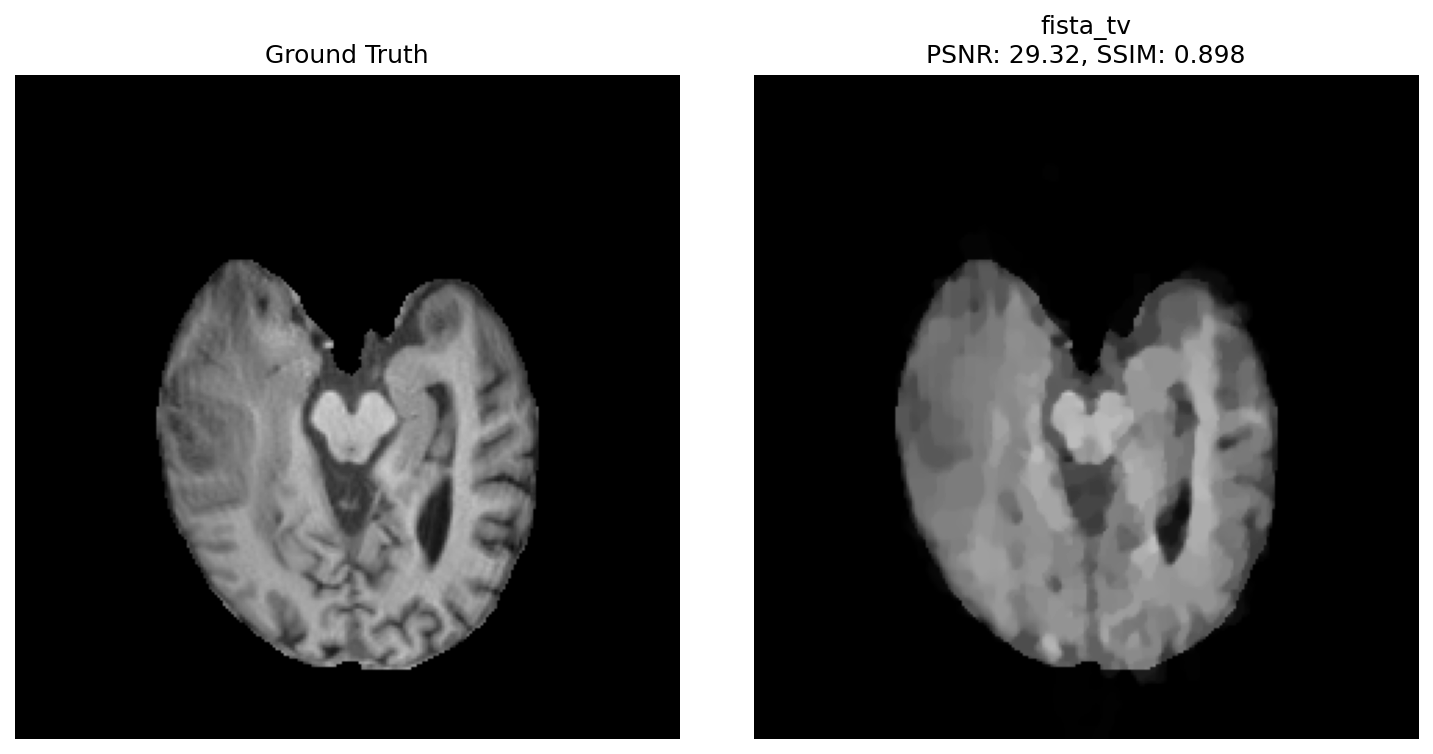
\includegraphics[trim={360pt 0 0 0}, clip,
        width=0.3\linewidth]{figs/fista_tv_batch0000.png} &
        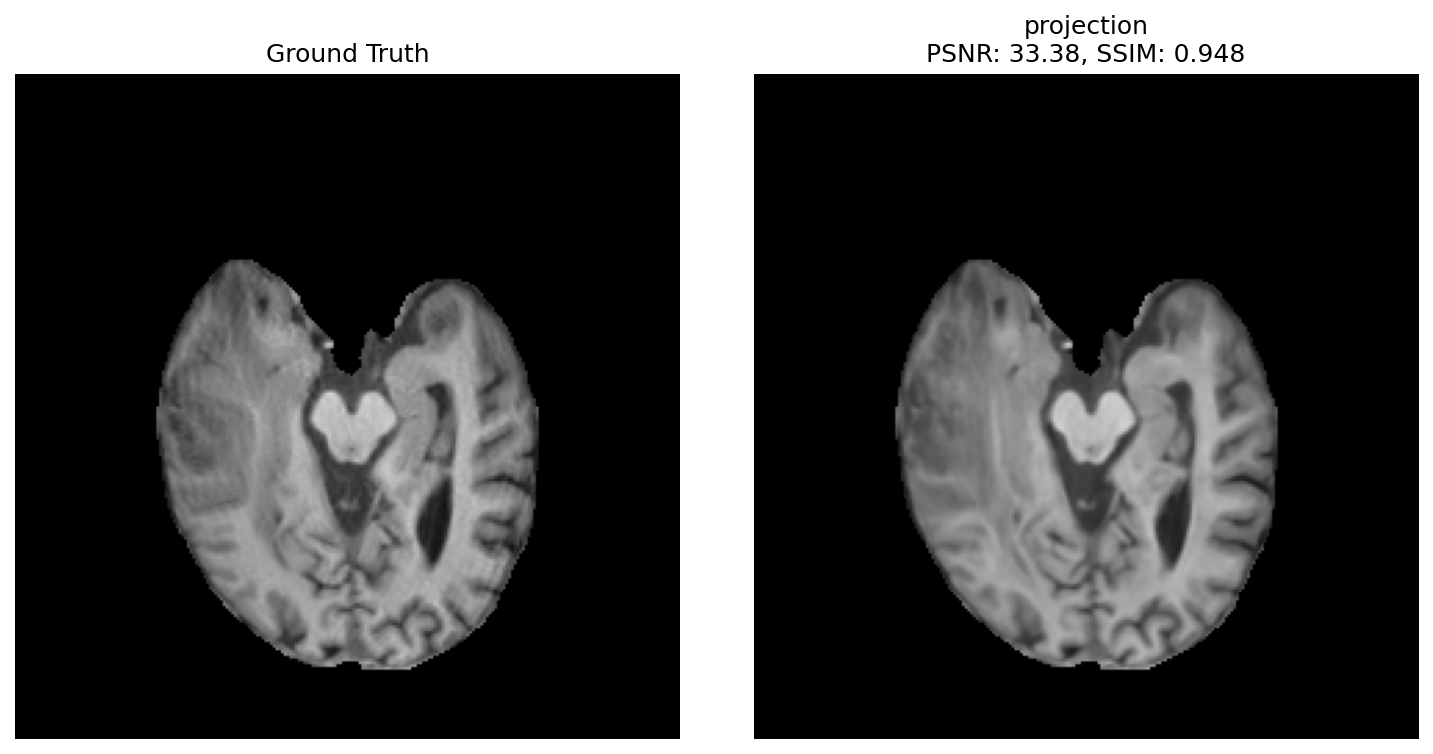
\includegraphics[trim={360pt 0 0 0}, clip,
        width=0.3\linewidth]{figs/projection_batch0000.png} &
        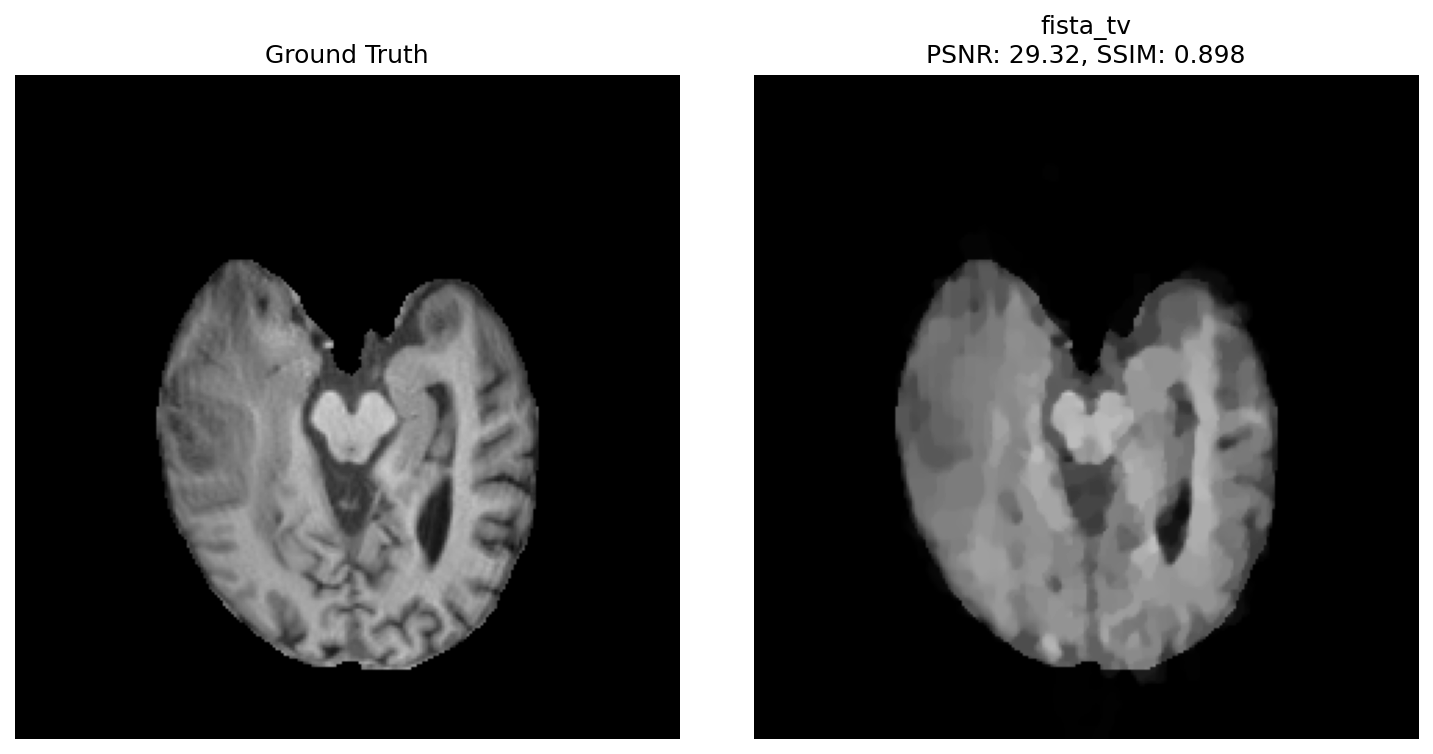
\includegraphics[trim={0 0 360pt 0}, clip,
        width=0.3\linewidth]{figs/fista_tv_batch0000.png} \\[2pt]
        % Row 2 - batch0002
        % 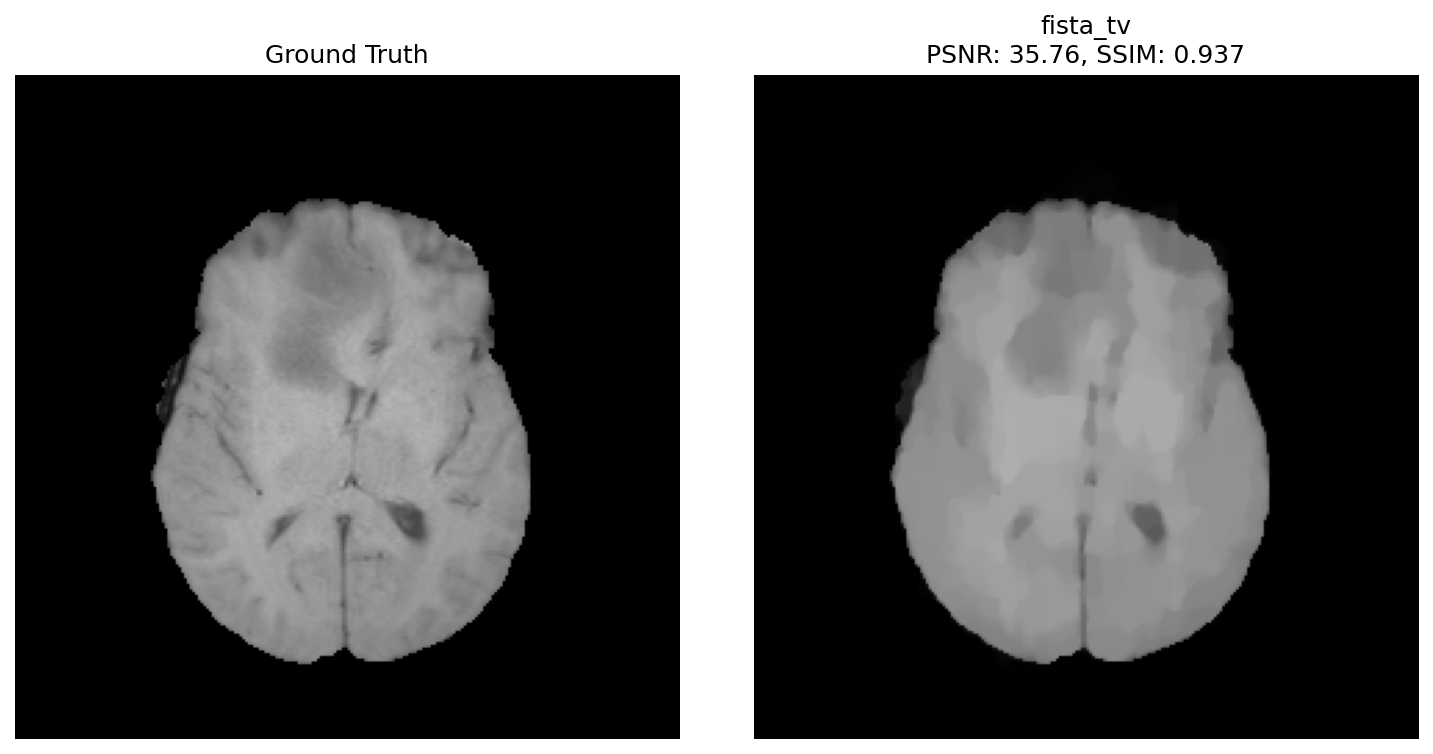
\includegraphics[trim={360pt 0 0 0}, clip,
        % width=0.3\linewidth]{figs/fista_tv_batch0002.png} &
        % 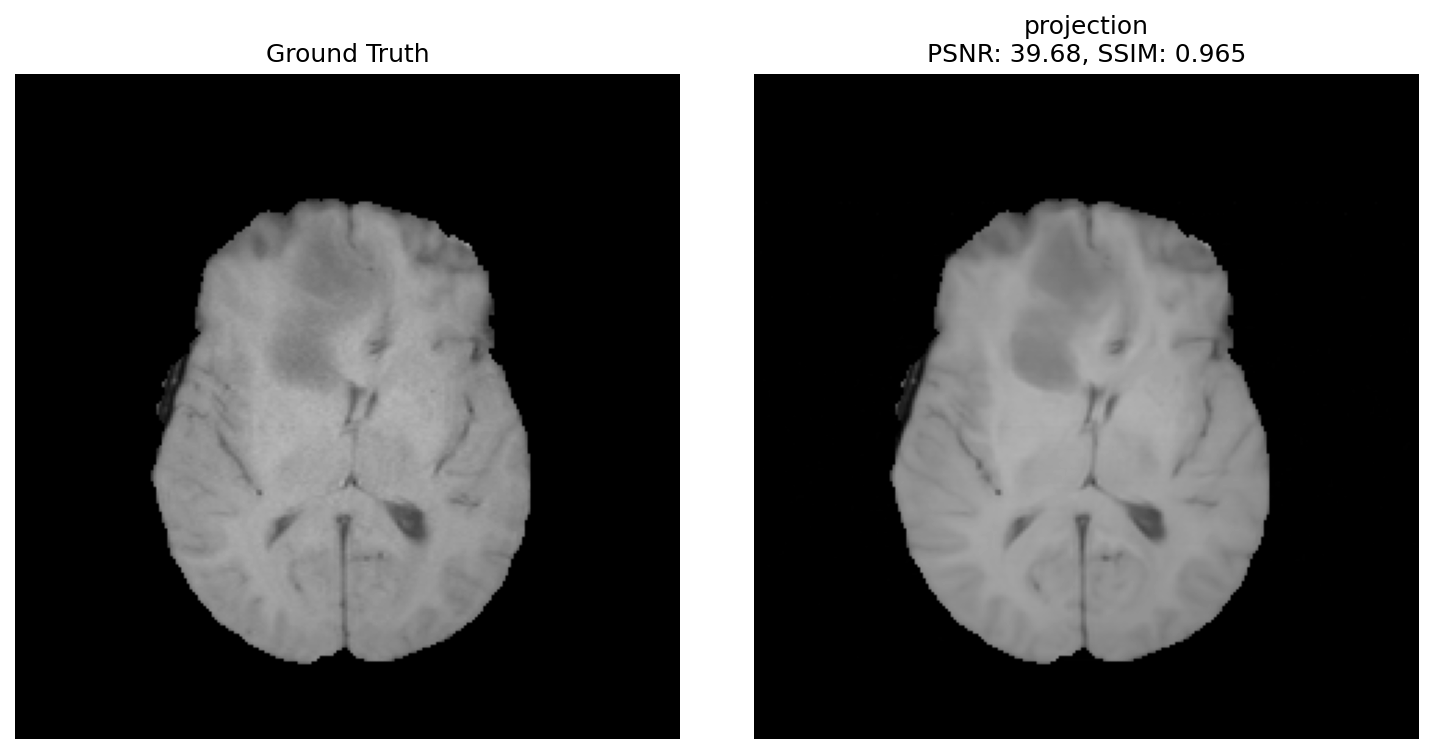
\includegraphics[trim={360pt 0 0 0}, clip,
        % width=0.3\linewidth]{figs/projection_batch0002.png} &
        % 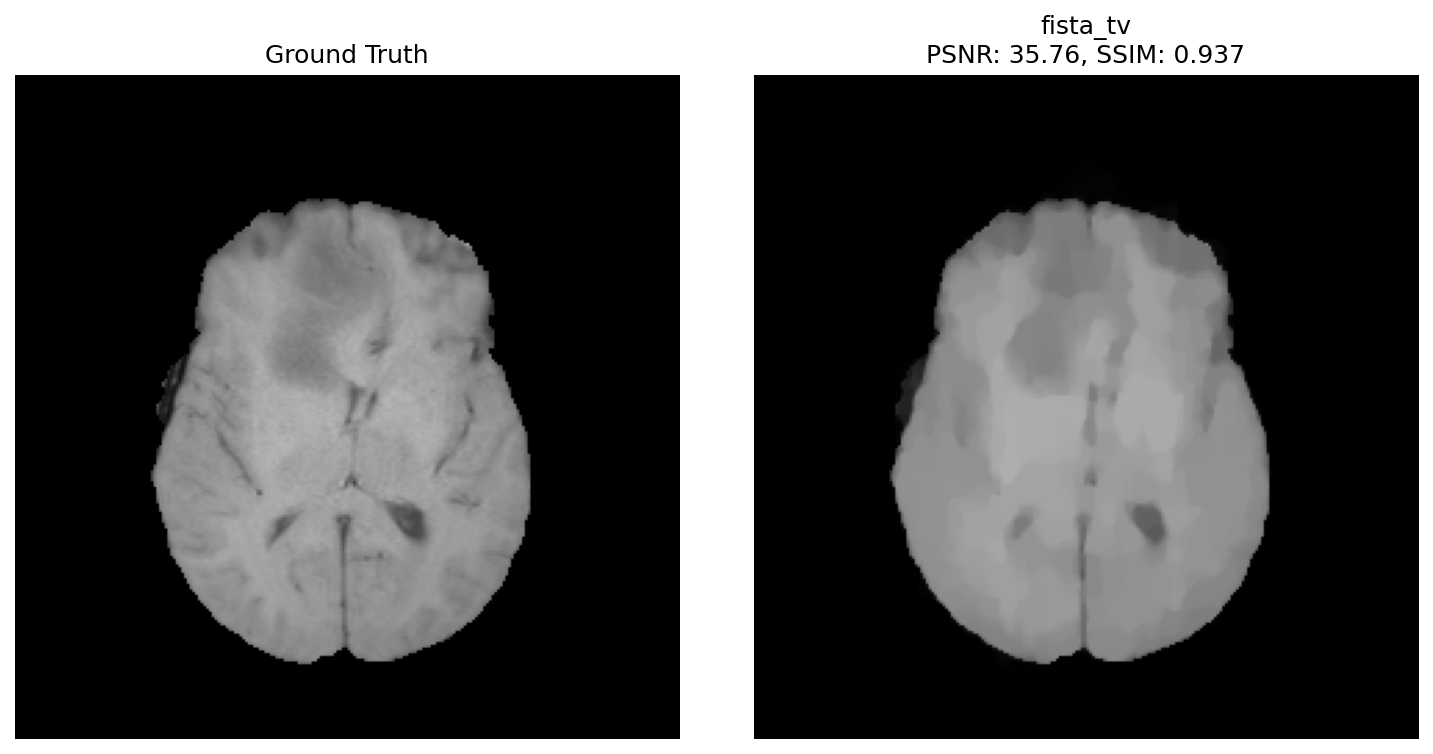
\includegraphics[trim={0 0 360pt 0}, clip,
        % width=0.3\linewidth]{figs/fista_tv_batch0002.png} \\[2pt]
        % Row 3 - batch0006
        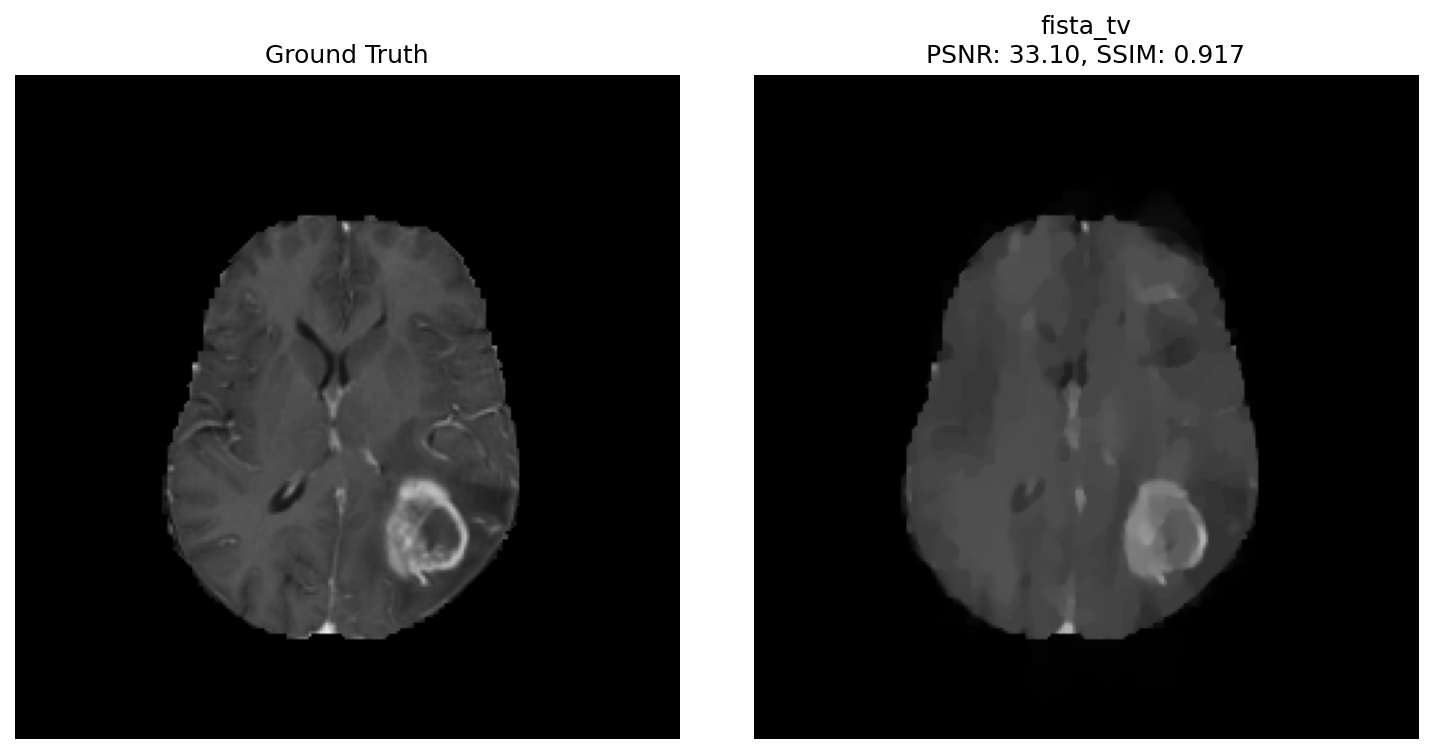
\includegraphics[trim={360pt 0 0 0}, clip,
        width=0.3\linewidth]{figs/fista_tv_batch0006.png} &
        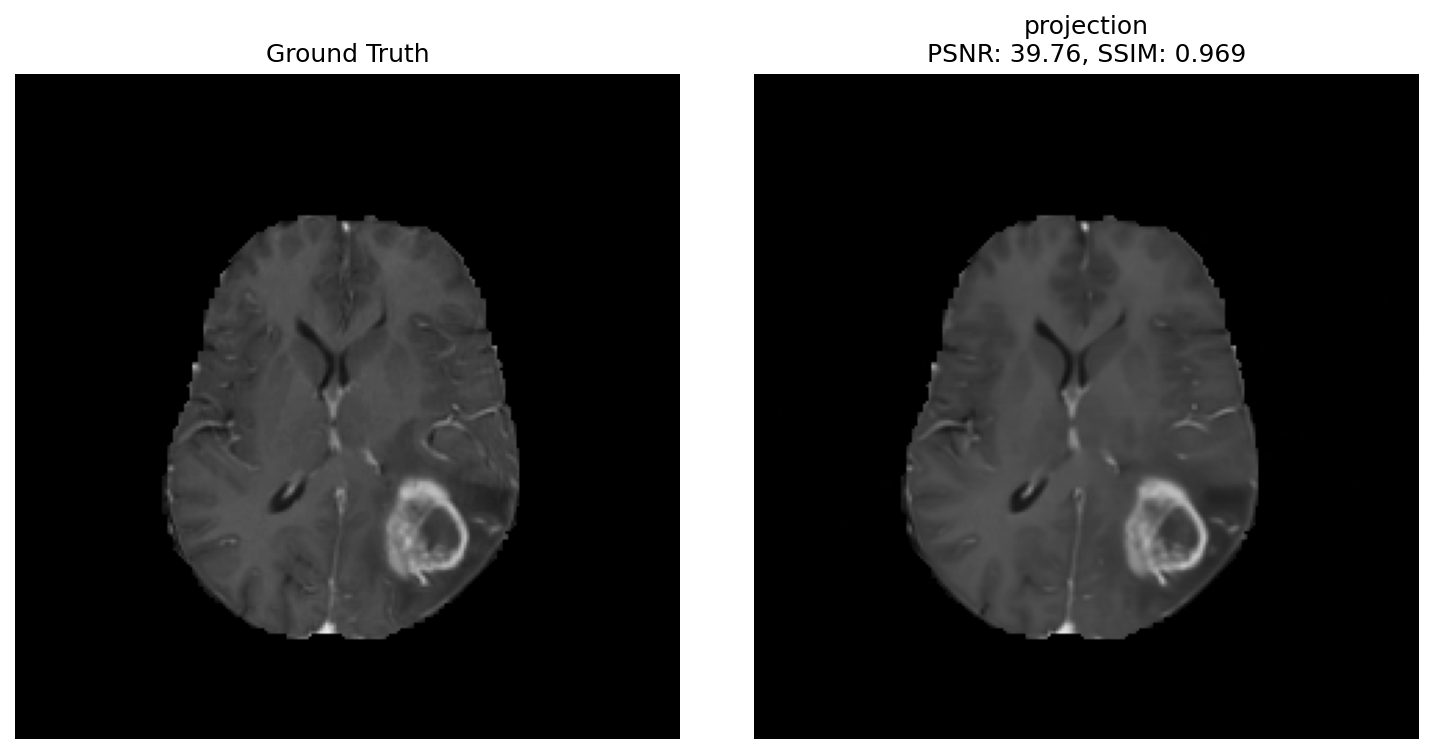
\includegraphics[trim={360pt 0 0 0}, clip,
        width=0.3\linewidth]{figs/projection_batch0006.png} &
        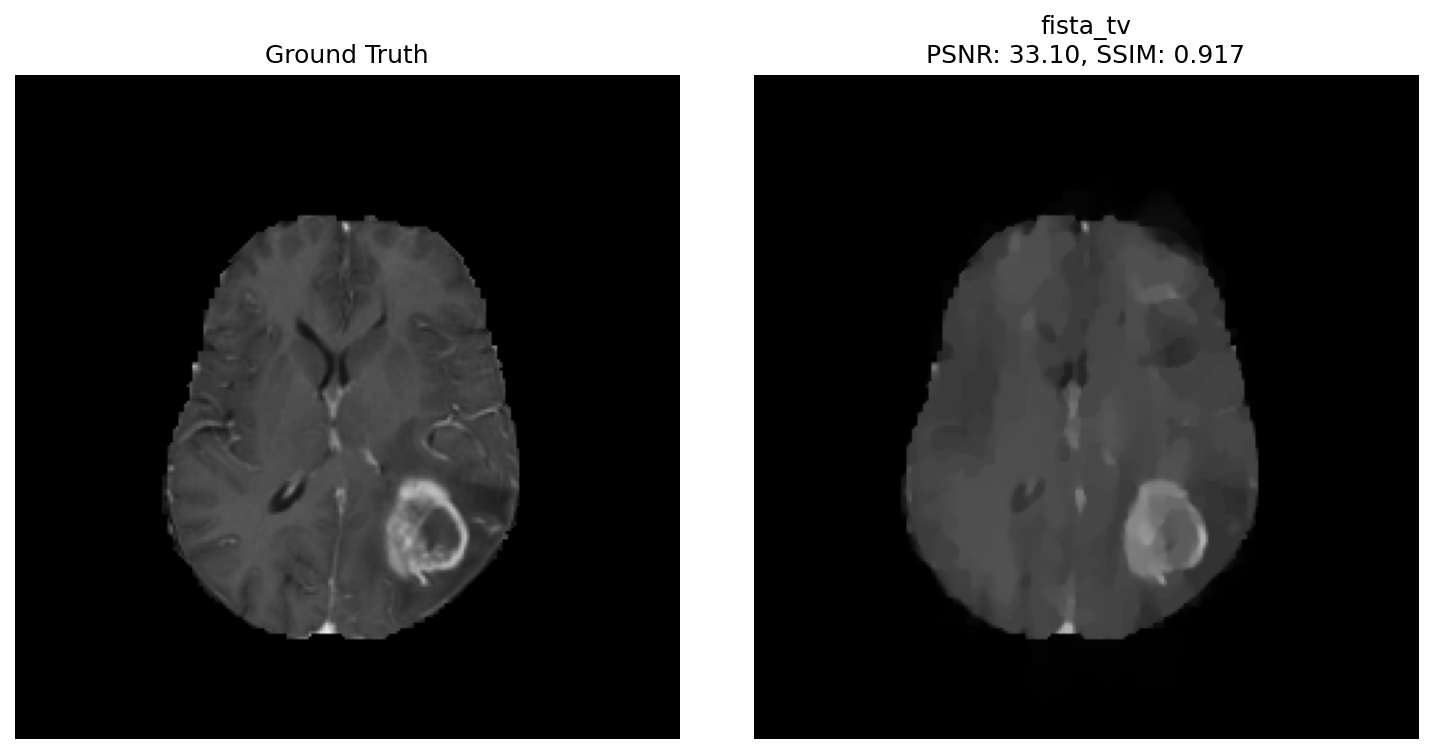
\includegraphics[trim={0 0 360pt 0}, clip,
        width=0.3\linewidth]{figs/fista_tv_batch0006.png}
    \end{tabular}
    \caption{\textbf{MRI 重建方法的视觉比较。}
        三个大脑 MRI 重建示例，展示了在 BraTS MRI 重建数据集上 8 倍欠采样下的 FISTA-TV、\textcite{song2022solving} 的测量一致性扩散方法以及真实图像。
        与 FISTA-TV 相比，基于扩散的方法产生的重建结果更接近真实结构，而 FISTA-TV 可以看出过度平滑了真实图像中存在的精细细节。同时，基于扩散的重建对真实图像的保真度（源于对测量一致性的适当强制执行）非常显著。}
    \label{fig:mri-reconstruction-visual}
\end{figure}

\begin{table}[t]
    \centering
    \begin{tabular}{@{}lccc@{}}
        \toprule
        Method & $24\times$ Accel. & $8\times$ Accel. & $4\times$ Accel. \\
        \midrule
        Cascade DenseNet & $23.39_{\pm 2.17}$ & $28.35_{\pm 2.30}$ &
        $30.97_{\pm 2.33}$ \\
        DuDoRNet & $18.46_{\pm 3.05}$ & $\bf 37.88_{\pm 3.03}$ &
        $30.53_{\pm 4.13}$ \\
        \textcite{song2020score} & $27.83_{\pm 2.73}$ & $35.04_{\pm
        2.11}$ & $37.55_{\pm 2.08}$ \\
        \textcite{NEURIPS2021_7d6044e9} & $28.80_{\pm 3.21}$ &
        $36.44_{\pm 2.28}$ & $38.76_{\pm 2.32}$ \\
        \textcite{song2022solving} & $\bf 29.42_{\pm 3.03}$ &
        $37.63_{\pm 2.70}$ & $\bf 39.91_{\pm 2.67}$ \\
        \bottomrule
    \end{tabular}
    \caption{\textbf{MRI 重建结果}，在 BraTS MRI 重建数据集上比较了不同加速因子（$\cS$ 中傅里叶空间子采样的程度）下的测量匹配方法。报告了带有标准差的 PSNR 指标（越高越好）。
        Cascade DenseNet
        \cite{NEURIPS2019_1e48c442} 和 DuDoRNet \cite{9156506} 是在 8 倍加速水平下在配对样本上训练的监督基线。最后三种方法是使用测量一致性的基于扩散的方法。
    经 \textcite{song2022solving} 许可复制。}
    \label{tab:mri-reconstruction}
\end{table}

\section{使用配对数据和测量的条件推断}
\label{sec:paired-data}
在许多实际应用中，我们既不知道感兴趣的数据 $\x$ 的分布，也不知道数据与其某些观测属性 $\y$ 之间的显式关系。我们只有一（大）组配对样本 $(\X, \Y) =
\{ (\x_1, \y_1), \ldots, (\x_N, \y_N) \}$，我们需要从中推断数据分布以及对它们之间关系进行建模的映射：
\begin{equation}
    h: \x \mapsto \y.
\end{equation}

图像分类问题可以看作是这样的一个例子。在某种意义上，分类问题是为自然图像学习一个（极度有损的）压缩编码器。例如，给定图像 $\x$ 的一个随机样本，我们希望预测其最能与 $\x$ 中内容相关的类别标签 $\y$。我们知道，与像素空间的维度相比，自然物体图像的分布是低维的。从前面的章节中我们了解到，在给定足够样本的情况下，原则上我们可以通过学习到的压缩编码为 $\x$ 学习一个结构化的低维表示 $\z$：
\begin{equation}
    f: \x \mapsto \z.
\end{equation}
表示 $\z$ 也可以被视为 $\x$ 的一个学习到的（有损但结构化的）代码。我们有理由假设，如果类别分配 $\y$ 真正依赖于 $\x$ 的低维结构，并且学习到的代码 $\z$ 真正反映了这种结构，那么 $\y$ 和 $\z$ 可以变得高度相关，因此它们的联合分布 $p(\z, \y)$ 应该是极度低维的。因此，我们可以将两个期望的代码 $\y$ 和 $\z$ 结合在一起，并尝试学习一个组合编码器：
\begin{equation}
    f: \x \mapsto (\z, \y)
\end{equation}
其中 $(\z, \y)$ 的联合分布是高度低维的。

根据我们在前面章节中的研究，映射 $f$ 通常被学习为同一空间中的一系列压缩或去噪算子。因此，为了利用这样一族操作，我们可以引入一个辅助向量 $\vw$，它可以被视为类别标签 $\y$ 的初始随机猜测。通过这种方式，我们可以学习一个压缩或去噪映射：
\begin{equation}\label{eq:classifier-with-class-token}
    f: (\x, \vw) \mapsto (\z, \y)
\end{equation}
在一个公共空间内。事实上，在用于分类任务的 Transformer（例如 ViT）训练中引入辅助“类别标记（class token）”的常见做法，可以被视为通过压缩给定（含噪）样本 $(\x, \vw)$ 的（编码率）来学习这样一种表示。如果数据 $\x$ 的分布已经是（低维）高斯混合分布，文献
\cite{wright2008classification} 已经表明，通过直接最小化与给定样本相关的\emph{（有损）编码长度}，可以有效地进行分类。

\subsection{类条件图像生成}\label{sub:cfg}
虽然学习到的分类器允许我们将给定图像 $\x$ 分类到其对应的类别，但我们通常希望通过对学习到的自然图像分布进行采样，来生成给定类别的图像。在某种程度上，这可以被视为图像分类的“逆”问题。令 $p_{\x}$ 表示自然图像的分布，例如由扩散-去噪过程建模。给定一个类别标签随机变量 $y \in [K]$ 及其实现 $\nu$，例如“苹果（Apple）”，我们希望对条件分布 $p_{\x \mid
y}(\,\cdot\, \mid \nu)$ 进行采样以生成一张苹果的图像：
\begin{equation}
    \hat{\x} \sim p_{\x\mid \y}(\,\cdot\, \mid \vnu).
\end{equation}
我们称之为\emph{类条件图像生成}。

在 \Cref{sec:conditioned-decoding} 中，我们已经看到了如何使用去噪-扩散范式，在给定\textit{基于模型}的测量 $\vy = h(\vx) + \vw$
（\Cref{eq:measurement-matching-observation}）的情况下从后验 $p_{\vx \mid \vy}$ 中进行条件采样，最终得到了
DPS 算法（\Cref{alg:iterative_denoising_conditional_DPS}）。这是一个强大的框架，但它不适用于此处的类（或文本）条件图像生成问题，因为由于解析建模的难解性，观测/属性 $y$ 的显式生成模型 $h$ 是不可用的。在本节中，我们将介绍将条件采样扩展到此设置的技术。

因此，我们现在仅假设我们可以访问来自 $(\vx, y)$ 联合分布的样本：
\begin{equation}
    (\vx, y) \sim p_{\vx, y}.
\end{equation}
与上一节一样，我们定义 $\vx_t = \alpha_t \vx + \sigma_t \vg$，其中 $\vg \sim \cN(\Zero, \vI)$ 独立于 $(\vx, \vy)$，如 \Cref{ch:denoising} 中的
\Cref{eq:gen_additive_gaussian_noise_model} 所示，并且我们将反复使用符号 $\vxi$ 来表示 $\vx$ 和 $\vx_t$ 的实现。

本节重点介绍现代生成模型中条件采样的概念和算法基础。有关各种应用中实现问题的讨论，请参见 \Cref{ch:applications} 的
\Cref{sec:cond_gen} 及后续小节。

\subsubsection{分类器引导：通过预训练分类器实现一致性}

% To proceed, we note that our development of conditional sampling under
% measurements $\vy = h(\vx) + \vw$ only explicitly used the
% forward model $h$ in making the DPS approximation
% \eqref{eq:conditional-posterior-measurementmatching-gaussian-case-dps-approx}.
回顾 \Cref{sec:conditioned-decoding}，由于贝叶斯法则以及给定 $\vx$ 时 $\vy$ 和 $\vx_t$ 的条件独立性（回顾
\Cref{fig:posterior-sampling-cds}），最优条件后验去噪器的以下分解成立：
% In particular, the conditional posterior denoiser decomposition
% \eqref{eq:posterior-sampling-denoiser-decomposition} \textit{still
% holds in the
% paired data setting},
\begin{equation}\label{eq:conditional-denoising-mmse-denoiser-paired-data}
    \bE[ \vx \mid \vx_t=\vxi, y=\nu]
    =
    \bE[\vx \mid \vx_t=\vxi]
    + \frac{\sigma_t^2}{\alpha_t}
    \nabla_{\vxi}\log p_{y \mid \vx_t}(\nu\mid \vxi).
\end{equation}
换句话说，无论显式观测模型 $\vy = h(\vx) + \vw$ 是否有效，最优条件去噪器的表示
\eqref{eq:conditional-denoising-mmse-denoiser-paired-data} 都成立。
这意味着，如果我们能在配对数据设置中学习到这样一个去噪器
\eqref{eq:conditional-denoising-mmse-denoiser-paired-data}，我们就可以遵循我们在
\Cref{ch:denoising} 中开发的去噪-扩散方法来执行类条件采样。

那么，一个自然的想法是使用参数为 $\theta_{\mathrm{c}}$ 的深度网络 $f_{\theta_{\mathrm{c}}}$ 直接实现
\eqref{eq:conditional-denoising-mmse-denoiser-paired-data} 中的似然校正项，如
\Cref{eq:classifier-with-class-token} 所示：
\begin{equation}
    f_{\theta_{\mathrm{c}}} : (t, \vx_t) \mapsto \softmax(\vW_{\mathrm{head}}
    \vz(t, \vx_t)).
\end{equation}
该表达式将含噪输入 $\vx_t$ 的最终表示 $\vz(t, \vx_t)$（它也依赖于
$\theta_{\mathrm{c}}$）与分类头 $\vW_{\mathrm{head}} \in \bR^{K
\times d}$ 结合起来，后者将表示映射到 $K$ 个可能类别的概率分布上。
正如实践中常见的那样，它还将加噪过程中的时间 $t$ 作为输入。
因此，通过适当的训练，它提供了对数似然
$\log p_{y \mid \vx_t}$ 的近似，并且对 $\log f_{\theta_{\mathrm{c}}}$ 关于其输入 $\vx_t$ 求导，可以得到
\Cref{eq:conditional-denoising-mmse-denoiser-paired-data} 中第二项的近似：
\begin{equation}\label{eq:conditional-denoising-mmse-denoiser-paired-data-approx}
    \bar{\vx}_{\theta}^{\mathrm{naive}}(t, \vx_t, y)
    =
    \bar{\vx}_{\theta_{\mathrm{d}}}(t, \vx_t)
    + \frac{\sigma_t^2}{\alpha_t}
    \nabla_{\vx_t}
    \ip*{
        \log f_{\theta_{\mathrm{c}}}(t, \vx_t)
    }{
        \ve_{y}
    }
\end{equation}
其中，像往常一样，我们通过一个参数为 $\theta_{\mathrm{d}}$ 的针对 $\vx_t$ 的学习到的无条件去噪器来近似
\Cref{eq:conditional-denoising-mmse-denoiser-paired-data} 中的第一项，并且我们将 $k \in [K]$ 的 $\ve_k$ 记为 $\R^K$ 的第 $k$ 个标准基向量（即第 $k$ 个位置为 1，其他位置为 0 的向量）。
读者应注意，条件去噪器 $\bar{\vx}_{\theta}$ 需要两次独立的训练运行，并具有独立的损失：一次是针对分类器参数 $\theta_{\mathrm{c}}$ 的分类损失，\footnote{在 \Cref{ch:applications} 中，我们详细回顾了训练此类分类器的过程。}另一次是针对去噪器参数
$\theta_{\mathrm{d}}$ 的去噪损失。这种条件采样方法在扩散模型的早期开创性工作中（特别是
\citet{Sohl-Dickstein2015} 和 \citet{song2020score} 的工作）已经被认识到并用于执行条件采样。

然而，这种直接的方法有两个主要缺点（这就是为什么我们将其标记为“朴素的”）。首先，根据经验，这样训练出来的深度网络分类器通常无法提供足够强的引导信号（在
\Cref{eq:conditional-denoising-mmse-denoiser-paired-data} 中）以确保生成的样本反映条件信息 $y$。这一点首先由 \citet{Dhariwal2021-hg} 强调，他们指出，在类条件 ImageNet 生成的设置中，学习到的深度网络分类器对于作为条件的类别 $y$ 的概率输出通常在
$0.5$ 左右——大到足以成为主导类别，但不足以提供强烈的引导信号——并且经检查，生成结果与条件类别 $y$ 并不一致。\citet{Dhariwal2021-hg} 提出通过启发式地将“逆温度”超参数 $\gamma > 0$
引入朴素条件去噪器
\eqref{eq:conditional-denoising-mmse-denoiser-paired-data-approx} 的定义中来解决这个问题，并将由此产生的条件去噪器称为结合了\textbf{“分类器引导”（Classifier Guidance, CG）}：
\begin{equation}\label{eq:conditional-denoising-mmse-denoiser-paired-data-approx-cg}
    \bar{\vx}_{\theta}^{\mathrm{CG}}(t, \vx_t, y)
    =
    \bar{\vx}_{\theta_{\mathrm{d}}}(t, \vx_t)
    + \gamma\frac{\sigma_t^2}{\alpha_t}
    \nabla_{\vx_t}
    \ip*{
        \log f_{\theta_{\mathrm{c}}}(t, \vx_t)
    }{
        \ve_{y}
    }
\end{equation}
其中 $\gamma = 1$ 的情况与
\eqref{eq:conditional-denoising-mmse-denoiser-paired-data-approx} 一致。

\citet{Dhariwal2021-hg} 发现，根据经验，设置 $\gamma > 1$ 表现最好。
对此的一种可能解释如下：请注意，在\textit{真实}似然项
\Cref{eq:conditional-denoising-mmse-denoiser-paired-data} 的上下文中，乘以 $\gamma$ 等价于
\begin{align}
    \gamma\frac{\sigma_t^2}{\alpha_t} \nabla_{\vxi}\log p_{\vy \mid
    \vx_t}(\vnu\mid
    \vxi)
    &=
    \frac{\sigma_t^2}{\alpha_t} \nabla_{\vxi}\log \left(
        p_{\vy \mid \vx_t}(\vnu\mid \vxi)^\gamma
    \right), %
\end{align}
这暗示了参数 $\gamma$ 对似然
$p_{\vy \mid \vx_t}$ 执行（逆）\textit{温度缩放}的自然解释，如果我们考虑重归一化分布
$ { p_{\vy \mid \vx_t}(\vnu\mid \vxi)^\gamma } / { \int p_{\vy \mid
    \vx_t}(\vnu'\mid
\vxi)^\gamma \odif \vnu' } $，这种解释是精确的。
然而，请注意，在 \Cref{eq:conditional-denoising-mmse-denoiser-paired-data} 的上下文中，这\textit{不是}一个严格的解释，因为梯度是关于 $\vxi$ 求的，而温度缩放分布中的归一化常数通常是 $\vxi$ 的函数。
相反，参数 $\gamma$ 应该简单地理解为放大了深度网络分类器输出概率
$f_{\theta_{\mathrm{c}}}(t, \vx_t)$ 中的较大值（\textit{相对于}较小值），这有效地放大了在深度
network $f$ assigns it the largest probability among the $K$ classes.

\subsubsection{通过无分类器引导的简化与改进}

尽管如此，分类器引导（classifier guidance）并没有解决朴素方法的第二个关键缺点：除了无条件去噪器 $\bar{\vx}_{\theta_{\mathrm{d}}}$ 之外，还必须训练一个辅助分类器 $f_{\theta_{\mathrm{c}}}$，这既繁琐又浪费，因为由于需要处理含噪输入 $\vx_t$ 并结合其他基于经验动机的架构修改，直接调整预训练分类器是不可能的。
特别是，\citet{Dhariwal2021-hg} 发现必须 \textit{显式地设计实现分类器的深度网络架构，使其与去噪器的架构相匹配}。

此外，纯粹从实用的角度来看——为了从生成的采样器中获得最佳性能——基于分类器引导的采样的最佳性能配置，甚至进一步偏离了我们上面提出的理想化且概念上合理的框架。
为了获得最佳性能，\citet{Dhariwal2021-hg} 发现有必要将类别标签 $y$ 作为额外输入提供给去噪器 $\bar{\vx}_{\theta_{\mathrm{d}}}$。因此，由 \citet{Dhariwal2021-hg} 推导出的理想化分类器引导去噪器 \eqref{eq:conditional-denoising-mmse-denoiser-paired-data-approx-cg}（正如我们上面从条件后验去噪器分解 \eqref{eq:conditional-denoising-mmse-denoiser-paired-data} 中推导的那样），并不能完全反映实践中性能最佳的去噪器——这种去噪器实际上是将给定 $y$ 时 $\vx_t$ 的 \textit{条件} 去噪器与来自辅助分类器的额外引导信号结合在了一起！

这种受经验驱动的现状，促使 \citet{Ho2022-ry} 在随后的工作中提出了一种在经验上更具实用性的方法，称为 \textbf{无分类器引导（classifier-free guidance, CFG）}。
他们没有将条件去噪器 \eqref{eq:conditional-denoising-mmse-denoiser-paired-data} 表示为 $\vx_t$ 的无条件去噪器与对数似然校正项的加权和（可能像分类器引导中那样修改了权重），而是接受了训练给定 $y$ 时 $\vx_t$ 的条件去噪器的明显必要性（正如 \citet{Dhariwal2021-hg} 的实验结果所证明的那样），并将对数似然梯度项替换为该条件去噪器与给定 $\vx_t$ 时 $\vx$ 的 \textit{无条件} 去噪器的正确加权和。\footnote{尽管如此，\textcite{Ho2022-ry} 实际上建议使用与我们在此处给出的不同的权重，这是基于 \textcite{Dhariwal2021-hg} 启发式地将 \eqref{eq:conditional-denoising-mmse-denoiser-paired-data} 中的无条件去噪器替换为条件去噪器这一事实。事实上，我们在此推导和给出的权重反映了现代实践，特别是被用于最先进的扩散模型中，例如 Stable Diffusion 3.5 \cite{DBLP:conf/icml/EsserKBEMSLLSBP24}。}

\paragraph{推导无分类器引导。} 为了解这种结构是如何产生的，我们从 \eqref{eq:conditional-denoising-mmse-denoiser-paired-data-approx-cg} 中定义的分类器引导去噪器 $\bar{\vx}_{\theta}^{\mathrm{CG}}$ 的“理想化”版本开始，对于该版本，去噪器 $\bar{\vx}_{\theta_{\mathrm{d}}}$ 和分类器 $f_{\theta_{\mathrm{c}}}$ 通过 \eqref{eq:conditional-denoising-mmse-denoiser-paired-data} 完美地逼近了它们的目标：
\begin{equation}\label{eq:conditional-denoising-mmse-denoiser-paired-data-exact-cg}
    \bar{\vx}_{\theta}^{\mathrm{CG,\,ideal}}(t, \vxi, \nu)
    =
    \bE[\vx \mid \vx_t=\vxi]
    + \gamma\frac{\sigma_t^2}{\alpha_t}
    \nabla_{\vxi}\log p_{y \mid \vx_t}(\nu\mid \vxi).
\end{equation}
然后我们使用贝叶斯法则，其形式为
\begin{equation}
    \log p_{y \mid \vx_t}
    =
    \log p_{\vx_t \mid y} + \log p_{y} - \log p_{\vx_t},
\end{equation}
结合 Tweedie 公式（\Cref{thm:tweedie}，如 \Cref{eq:gen_tweedie} 中所修改）在得分函数和去噪器之间进行转换，得到
\begin{align*}
    \bar{\vx}_{\theta}^{\mathrm{CG,\,ideal}}(t, \vxi, \nu)
    &=
    \frac{1}{\alpha_t} \vxi
    + (1-\gamma) \frac{\sigma_t^2}{\alpha_t}
    \nabla_{\vxi}\log p_{\vx_t}(\vxi)
    + \gamma \frac{\sigma_t^2}{\alpha_t}
    \nabla_{\vxi}\log p_{\vx_t \mid y}(\vxi \mid \nu)
    \\
    &=
    (1 - \gamma) \bE[\vx \mid \vx_t=\vxi]
    +
    \gamma \bE[\vx \mid \vx_t=\vxi, y=\nu],
    \labelthis\label{eq:ideal-cfg-denoiser}
\end{align*}
其中在最后一行，我们应用了 \Cref{eq:conditional-denoising-conditioning-order-irrelevant}。
现在，\Cref{eq:ideal-cfg-denoiser} 提出了一种自然的近似策略：如前所述，我们将给定 $\vx_t$ 时 $\vx$ 的已学习无条件去噪器，与给定 $\vx_t$ 和 $y$ 时 $\vx$ 的已学习 \textit{条件} 去噪器结合起来。

然而，遵循 \textcite{Ho2022-ry} 以及训练深度网络去噪器的常见实践，标准的做法是使用 \textit{同一个} 深度网络来同时表示条件去噪器和无条件去噪器，方法是引入一个额外的标签（我们将其记为 $\varnothing$）来表示“无条件”情况。
这导出了 CFG 去噪器的形式：
\begin{equation}\label{eq:conditional-denoising-mmse-denoiser-paired-data-approx-cfg}
    \bar{\vx}_{\theta}^{\mathrm{CFG}}(t, \vx_t, y)
    =
    (1 - \gamma) \bar{\vx}_{\theta}(t, \vx_t, \varnothing)
    +
    \gamma \bar{\vx}_{\theta}(t, \vx_t, y).
\end{equation}
为了训练一个用于无分类器引导采样的去噪器 $\bar{\vx}_{\theta}(t, \vx_t, y^+)$，其中 $y^+ \in \set{1, \dots, K, \varnothing}$，我们的过程与 \Cref{alg:learning_denoiser} 中的无条件训练过程几乎完全相同，但有两个修改：
\begin{enumerate}
    \item 当我们从数据集中采样时，我们采样一个数据对 $(\vx, y)$，而不仅仅是一个样本 $\vx$。
    \item 每次我们从数据集中采样一个数据对时，我们通过以下方式采样增广标签 $y^+$：
        \begin{equation}
            y^+ =
            \begin{cases}
                \varnothing & \text{with probability } p_{\mathrm{uncond}}; \\
                y & \text{else}.
            \end{cases}
        \end{equation}
        此处，$p_{\mathrm{uncond}} \in [0, 1]$ 是一个新的超参数。这可以被视为一种 dropout 形式 \cite{srivastava2014dropout}。
\end{enumerate}
通过这种方式，我们训练了一个适用于无分类器引导采样的条件去噪器。我们在 \Cref{alg:iterative_denoising_conditional_CFG} 中总结了使用无分类器引导进行类条件采样的整体采样过程。

\begin{algorithm}
    \caption{使用分类数据和类条件去噪器进行条件采样。}
    \label{alg:iterative_denoising_conditional_CFG}
    \begin{algorithmic}[1]
        \Require{用于采样的有序时间步列表 \(0 \leq t_{0} < \cdots < t_{L} \leq T\)。}
        \Require{作为条件的类别标签 $\nu \in \set{1, \dots, K}$。}
        \Require{针对 $p_{\vx \mid y}$ 和 $p_{\vx}$ 的去噪器 \(\bar{\vx}_{\theta} \colon \{t_{\ell}\}_{\ell = 1}^{L} \times \R^{D} \times \set{1, \dots, K, \varnothing} \to \R^{D}\)（对于 $p_{\vx}$ 输入 $\varnothing$）。}
        \Require{尺度和噪声水平函数 \(\alpha, \sigma \colon \{t_{\ell}\}_{\ell = 0}^{L} \to \R_{\geq 0}\)。}
        \Require{引导强度 $\gamma \geq 0$（为了性能通常首选 $\gamma > 1$）。}
        \Ensure{一个样本 \(\hat{\vx}\)，近似服从 \(p_{\vx \mid y}(\,\cdot\, \mid \nu)\)。}
        \Function{DDIMSamplerConditionalCFG}{$\bar{\vx}_{\theta}, \nu, \gamma, (t_{\ell})_{\ell = 0}^{L}$}
        \State{初始化 \(\hat{\vx}_{t_{L}} \sim\) \(\vx_{t_{L}}\) 的近似分布（VP \(\implies \dNorm(\vzero, \vI)\)，VE \(\implies \dNorm(\vzero, t_{L}^{2}\vI)\)）。}
        \For{\(\ell = L, L - 1, \dots, 1\)}
        \State{计算
            \begin{equation*}
                \hat{\vx}_{t_{\ell - 1}} \doteq \frac{\sigma_{t_{\ell - 1}}}{\sigma_{t_{\ell}}}\hat{\vx}_{t_{\ell}} + \bp{\alpha_{t_{\ell - 1}} - \frac{\sigma_{t_{\ell - 1}}}{\sigma_{t_{\ell}}}\alpha_{t_{\ell}}}\bigl( (1 - \gamma) \bar{\vx}_{\theta}(t_{\ell}, \hat{\vx}_{t_{\ell}}, \varnothing) + \gamma \bar{\vx}_{\theta}(t_{\ell}, \hat{\vx}_{t_{\ell}}, \nu) \bigr)
            \end{equation*}
        }
        \EndFor
        \State{\Return{\(\hat{\vx}_{t_{0}}\)}}
        \EndFunction
    \end{algorithmic}
\end{algorithm}

\textcite{Ho2022-ry} 报告了使用无分类器引导进行类条件图像生成的强大经验性能，它已成为最大规模的实用扩散模型（如 Stable Diffusion \cite{rombach2022high} 及其衍生模型）的支柱。

\paragraph{无分类器引导促进学习什么样的去噪器？}
正如我们所见，无分类器引导的推导相当不透明且受经验驱动，几乎没有提供关于其强大性能背后机制的深入见解。
许多理论工作试图解决这个问题 \cite{Bradley2024-jg,Li2025-li,Wu2024-js}。
它们为整体 CFG 方法的某些部分提供了理论解释——该方法本身涵盖了去噪器的参数化和训练，以及采样时引导强度和性能的配置。
下面，遵循本书贯穿始终的主题，我们将在高斯混合模型数据分布和去噪器的简化设置中给出一种解释。
首先，我们考虑 \textit{CFG 的作用}：较大的权重 $\gamma \gg 1$ 会促进什么？

% \yima{请使下面示例试图传达的信息更加模块化。也许可以将其分成两个相关的部分？}
\begin{example}\label{example:denoising-gaussian-mixture-cfg}
    回顾我们在 \Cref{example:denoising_gaussian_mixture} 中研究的低秩高斯混合数据生成过程（特别是 \Cref{eq:MoG1} 中的形式）。给定 $K \in \bN$ 个类别，我们假设
    \begin{equation}\label{eq:MoG1-ch6}
        \vx \sim \frac{1}{K}\sum_{k = 1}^{K}\dNorm(\vzero,
        \vU_{k}\vU_{k}^{\top}),
    \end{equation}
    其中每个 \(\vU_{k} \in \O(D, P) \subseteq \R^{D \times P}\) 是一个具有正交列的矩阵，且 $P \ll D$。
    此外，我们假设类别标签 $y \in [K]$ 是 $\vx$ 的确定性函数，将样本映射到其对应的混合分量。
    我们考虑在 \Cref{ch:denoising} 中研究的简单噪声过程 \eqref{eq:additive_gaussian_noise_model}，因此对于所有 $t \in [0, T]$，有 $\vx_t = \vx + t \vg$，其中 $\vg \sim \cN(\Zero, \vI)$。

    应用 \Cref{example:denoising_gaussian_mixture} 中的分析（以及随后对低秩情况的分析，最终得出 \Cref{eq:gmm_lowrank_denoiser}），我们得到类条件最优去噪器为
    \begin{equation}\label{eq:gmm_lowrank_denoiser-ch6-classcond}
        \bE[ \vx \mid \vx_t = \vxi, y = \nu ]
        = \frac{1}{1 + t^{2}}
        \vU_{\nu}\vU_{\nu}^{\top}\vxi
    \end{equation}
    对于每个 $\nu \in [K]$，而对于最优无条件去噪器，我们得到
    \begin{equation}\label{eq:gmm_lowrank_denoiser-ch6-uncond}
        \bE[ \vx \mid \vx_t = \vxi ]
        = \frac{1}{1 + t^{2}}\sum_{k =
        1}^{K}\frac{\exp\rp{\frac{1}{2t^{2}(1 +
        t^{2})}\norm{\vU_{k}^{\top}\vxi}_{2}^{2}}}{\sum_{i =
            1}^{K}\exp\rp{\frac{1}{2t^{2}(1 +
        t^{2})}\norm{\vU_{i}^{\top}\vxi}_{2}^{2}}}\vU_{k}\vU_{k}^{\top}\vxi.
    \end{equation}
    因此，我们可以将引导强度为 $\gamma > 1$ 的 CFG 去噪器表示为
    \begin{equation}\label{eq:cfg-denoiser-mog-low-rank}
        \begin{split}
            \bar{\vx}^{\mathrm{CFG,\,ideal}}(t, \vx_t, y)
            =
            \frac{1}{1 + t^{2}}
            \Biggl(
                &(1 - \gamma)
                \sum_{k = 1}^{K}\frac{\exp\rp{\frac{1}{2t^{2}(1
                + t^{2})}\norm{\vU_{k}^{\top}\vx_t}_{2}^{2}}}{\sum_{i
                    = 1}^{K}\exp\rp{\frac{1}{2t^{2}(1
                                +
                t^{2})}\norm{\vU_{i}^{\top}\vx_t}_{2}^{2}}}\vU_{k}\vU_{k}^{\top}
                \\
                &\qquad+
                \gamma
                \vU_{y}\vU_{y}^{\top}
            \Biggr)
            \vx_t.
        \end{split}
    \end{equation}

    该去噪器具有简单、可解释的形式：
    \begin{enumerate}
        \item 第一项对应于 \textit{无条件去噪器}，它对信号 $\vx_t$ 进行去噪，去噪目标是与每个子空间相关的去噪器的平均值，其权重由 $\vx_t$ 与每个子空间的相关程度决定。
        \item 第二项对应于 \textit{条件去噪器}，它简单地使用条件类别的去噪器进行去噪。
    \end{enumerate}

    CFG 方案对这两个去噪器进行平均。这种平均的效果可以从以下重构中看出
    \begin{equation}\label{eq:cfg-denoiser-mog-low-rank-2}
        \begin{split}
            \bar{\vx}^{\mathrm{CFG,\,ideal}}(t, \vx_t, y)
            =
            \frac{1}{1 + t^{2}}
            &\Biggl(
                \left[\gamma + (1 - \gamma)
                    \frac{\exp\rp{\frac{1}{2t^{2}(1
                    + t^{2})}\norm{\vU_{y}^{\top}\vx_t}_{2}^{2}}}{\sum_{i
                        = 1}^{K}\exp\rp{\frac{1}{2t^{2}(1
                    + t^{2})}\norm{\vU_{i}^{\top}\vx_t}_{2}^{2}}}
                \right]
                \vU_{y}\vU_{y}^{\top}
                \\
                &\quad+
                (1 - \gamma)
                \sum_{k \neq y}\frac{\exp\rp{\frac{1}{2t^{2}(1
                + t^{2})}\norm{\vU_{k}^{\top}\vx_t}_{2}^{2}}}{\sum_{i
                    = 1}^{K}\exp\rp{\frac{1}{2t^{2}(1
                                +
                t^{2})}\norm{\vU_{i}^{\top}\vx_t}_{2}^{2}}}\vU_{k}\vU_{k}^{\top}
            \Biggr)
            \vx_t,
        \end{split}
    \end{equation}
    其中我们将条件去噪器与 $k \in [K]$ 求和中对应的 $k=y$ 项结合在一起。
    我们有
    \begin{equation}
        \sum_{k=1}^K
        \frac{\exp\rp{\frac{1}{2t^{2}(1
        + t^{2})}\norm{\vU_{k}^{\top}\vx_t}_{2}^{2}}}{\sum_{i
            = 1}^{K}\exp\rp{\frac{1}{2t^{2}(1
        + t^{2})}\norm{\vU_{i}^{\top}\vx_t}_{2}^{2}}}
        = 1,
    \end{equation}
    并且每个加数都是非负的，因此其上界也为 $1$。
    因此，我们可以得出 \Cref{eq:cfg-denoiser-mog-low-rank-2} 中各项的两种状态（regimes）：
    \begin{enumerate}
        \item \textbf{高相关状态：} 在这种情况下，假设含噪输入 $\vx_t$ 与其中一个子空间 $\vU_y$ 高度相关。如果 $\vx_t$ 与 $\vU_y$ 高度相关，那么无条件去噪器中对应于 $k=y$ 加数的归一化权重接近于 $1$。那么
            \begin{equation}
                \gamma + (1 - \gamma)
                \frac{\exp\rp{\frac{1}{2t^{2}(1
                + t^{2})}\norm{\vU_{y}^{\top}\vx_t}_{2}^{2}}}{\sum_{i
                    = 1}^{K}\exp\rp{\frac{1}{2t^{2}(1
                + t^{2})}\norm{\vU_{i}^{\top}\vx_t}_{2}^{2}}}
                \approx 1,
            \end{equation}
            所有其他权重必然接近于零，并且 CFG 去噪器近似等于与条件类别 $y$ 相关的去噪器。

            这意味着：\textit{如果 CFG 去噪器的输入与某个类别子空间高度相关，则该去噪器近似等于相应的类条件去噪器}！因此，我们期望 CFG 去噪采样器能够收敛。
        \item \textbf{低相关状态：} 相反，如果 $\vx_t$ 与 $\vU_y$ \textit{不} 高度相关（例如因为 $t$ 很大），那么无条件去噪器中对应于 $k=y$ 加数的归一化权重接近于 $0$。结果，
            \begin{equation}
                \gamma + (1 - \gamma)
                \frac{\exp\rp{\frac{1}{2t^{2}(1
                + t^{2})}\norm{\vU_{y}^{\top}\vx_t}_{2}^{2}}}{\sum_{i
                    = 1}^{K}\exp\rp{\frac{1}{2t^{2}(1
                + t^{2})}\norm{\vU_{i}^{\top}\vx_t}_{2}^{2}}}
                \approx \gamma,
            \end{equation}
            因此，引导强度 $\gamma \gg 1$ 会在与 $y$ 相关的去噪器上施加一个很大的正权重。

            同时，在 \Cref{eq:cfg-denoiser-mog-low-rank-2} 的第二项中，任何与 $\vx_t$ 高度相关的类别 $k \neq y$ 都会从 $1 - \gamma$ 系数中获得一个很大的 \textit{负} 权重。
            这同时产生了一种效果：使去噪后的信号与条件类别 $y$ 的相关性大幅增加，并使其与前一次迭代（即去噪前的迭代）呈负相关。

            换句话说，\textit{CFG 引导迭代去噪过程朝向条件类别并远离前一次迭代}，这是一种不同于纯条件采样（即 $\gamma = 1$ 的情况）的动力学机制。
    \end{enumerate}
\end{example}

\Cref{example:denoising-gaussian-mixture-cfg} 表明，在高斯混合设置中，CFG 去噪器提供了对条件类别的强烈偏置，同时在噪声水平 $t$ 较小时保持了局部正确性（从而保证了采样的收敛性）。
这提示了为什么在实践中发现较大的权重 $\gamma \gg 1$ 是必不可少的。

接下来，下面的示例将展示在存在低维结构的情况下，对去噪器 \textit{参数化} 的深入见解，同样是在高斯混合模型中。

\begin{example}\label{example:denoising-gaussian-mixture-cfg-parameterization}
    再次考虑在 \Cref{example:denoising-gaussian-mixture-cfg} 中研究的高斯混合模型：
    \begin{equation}
        \vx \sim \frac{1}{K}\sum_{k = 1}^{K}\dNorm(\vzero,
        \vU_{k}\vU_{k}^{\top}),
    \end{equation}
    其中每个 \(\vU_{k} \in \O(D, P) \subseteq \R^{D \times P}\) 是一个具有正交列的矩阵，且 $P \ll D$。
    类别标签 $y \in [K]$ 是 $\vx$ 的确定性函数，将样本映射到其对应的混合分量。
    对于该分布，并且再次在 \Cref{ch:denoising} 中研究的简单噪声过程 \eqref{eq:additive_gaussian_noise_model} 下（其中对于所有 $t \in [0, T]$ 有 $\vx_t = \vx + t \vg$，且 $\vg \sim \cN(\Zero, \vI)$），我们在 \Cref{example:denoising-gaussian-mixture-cfg} 中看到理想的 CFG 去噪器具有以下形式
    \begin{equation}\label{eq:cfg-denoiser-mog-low-rank-3}
        \begin{split}
            \bar{\vx}^{\mathrm{CFG,\,ideal}}(t, \vx_t, y)
            =
            \frac{1}{1 + t^{2}}
            \Biggl(
                &(1 - \gamma)
                \sum_{k = 1}^{K}\frac{\exp\rp{\frac{1}{2t^{2}(1
                + t^{2})}\norm{\vU_{k}^{\top}\vx_t}_{2}^{2}}}{\sum_{i
                    = 1}^{K}\exp\rp{\frac{1}{2t^{2}(1
                                +
                t^{2})}\norm{\vU_{i}^{\top}\vx_t}_{2}^{2}}}\vU_{k}\vU_{k}^{\top}
                \\
                &\qquad+
                \gamma
                \vU_{y}\vU_{y}^{\top}
            \Biggr)
            \vx_t.
        \end{split}
    \end{equation}

    % 我们现在对这种引导去噪器的形式进行进一步分析，以
    % 便对 CFG 的作用做出一些推论。
    % % 其中许多见解
    % % 也将与具有低维几何结构的 \textit{一般} 数据分布相关。
    % % 
    % 首先，请注意 CFG 去噪器 \eqref{eq:cfg-denoiser-mog-low-rank-3}
    % 在 $\vx_t$ 与单个子空间 $\vU_y$ 的相关性明显强于
    % 任何其他 $\vU_{y'}$ 的设置中采取简单的形式。实际上，
    % 因为类条件去噪器中的权重比由下式给出
    % \begin{equation}
    %     \frac{
    %         \exp\rp{\frac{1}{2t^{2}(1 +
    %         t^{2})}\norm{\vU_{y}^{\top}\vx_t}_{2}^{2}}
    %     }{
    %         \exp\rp{\frac{1}{2t^{2}(1 +
    %         t^{2})}\norm{\vU_{y'}^{\top}\vx_t}_{2}^{2}}
    %     }
    %     =
    %     \exp\rp{
    %         \frac{1}{2t^{2}(1 + t^{2})}\left(
    %             \norm{\vU_{y}^{\top}\vx_t}_{2}^{2}
    %             -
    %             \norm{\vU_{y'}^{\top}\vx_t}_{2}^{2}
    %         \right)
    %     },
    % \end{equation}
    % $\vx_t$ 与 $\vU_{y}$ 的相关性同其他子空间 $\vU_{y'}$ 的相关性之间存在巨大差距，
    % 这意味着对 $k$ 的求和集中在 $k=y$ 的加数上，
    % 从而得出 \textit{CFG 去噪器仍然等于
    % 类条件去噪器}。此外，当 $t \approx 0$ 时，
    % 任何这种差距都会在指数中被放大，使得这种对
    % $k=y$ 加数的集中更加强烈。特别是，对于较小的时间 $t$（即接近
    % 数据分布的支撑集），CFG 去噪与
    % 标准的类条件去噪没有区别——这意味着一旦它达到这种配置，
    % 它将稳定收敛。
    % 因此，CFG 的经验优势应该归功于它在
    % $\vx_t$ 并非明确来自单一类别的情况下的行为。

    现在我们考虑参数化一个可学习的去噪器 $\vx_{\theta}^{\mathrm{CFG}}$ 以表示最优去噪器 \eqref{eq:cfg-denoiser-mog-low-rank-3} 的问题。
    % 在这里，最初可能看起来混合分布的分类设置
    % 相对于学习实际数据分布来说过于特殊，
    % 因为理想的去噪器 \eqref{eq:cfg-denoiser-mog-low-rank-3} 在
    % 这种设置下具有简单的形式，即含噪信号 $\vx_t$ 到
    % 对应于 $\vx$ 的真实类别标签 $y$ 的子空间 $\vU_y$（相关的去噪器）的 \textit{硬分配}，
    % 并与所有子空间 $\vU_k$ 相关的 \textit{软分配} 去噪器进行平均，
    % 其权重由 $\vx_t$ 与这些不同子空间的相关性给出。
    % 然而，我们可以为这个例子中的类条件去噪器提取一个更一般的形式，
    % 这与使用高斯混合分布的几何结构进行实际参数化相关，
    % 它实际上与现实世界数据中常见的几何结构类型相似。
    % 更准确地说，
    为了易于处理，我们添加了一个与子空间 $\vU_k$ 彼此“可区分”相关的额外假设，这在实践中是很自然的：具体来说，我们假设对于任何一对索引 $k, k' \in [K]$ 且 $k \neq k'$，我们可以找到一组 $K$ 个非零方向 $\vv_{k} \in \bR^D$，使得
    \begin{equation}
        \vU_{k}\vU_{k}^\top \vv_k = \vv_k, \quad
        \vU_{k'}\vU_{k'}^\top \vv_k = \Zero, \enspace k' \neq k.
    \end{equation}
    这是一个比简单的可区分性稍强的假设，但应该注意的是，它并没有过度限制：例如，它仍然允许子空间 $\vU_{k}$ 彼此之间具有显著的相关性。\footnote{更一般地说，这个假设自然地被表述为子空间 $\vU_{[K]}$ 之间的 \textit{不相干条件（incoherence condition）}，这在压缩感知理论中很常见 \cite{Wright-Ma-2022}。}

    然后，这些向量 $\vv_k$ 可以被认为是类别标签 $y \in [K]$ 的 \textit{嵌入（embeddings）}，我们可以使用它们来定义一个更一般的算子，该算子可以同时表示无条件去噪器和类条件去噪器。更准确地说，考虑映射
    \begin{equation}\label{eq:mog-conditional-denoising-unified-operator}
        (\vx_t, \vv) \mapsto
        \sum_{k = 1}^{K}\frac{
            \exp\rp{\frac{1}{2t^{2}(1
            + t^{2})} \abs{\vx_t^\top \vU_k \vU_k^\top \vv}}
        }
        {
            \sum_{i
            = 1}^{K}\exp\rp{\frac{1}{2t^{2}(1
            + t^{2})}\abs{\vx_t^\top \vU_i \vU_i^\top \vv}}
        }
        \vU_{k}\vU_{k}^{\top}\vx_t.
    \end{equation}
    那么，如果我们将 $\vv = \vx_t$ 代入算子 \eqref{eq:mog-conditional-denoising-unified-operator}，我们会得到一个与 \eqref{eq:gmm_lowrank_denoiser-ch6-uncond} 中第一项成正比的结果，对应于 $\vx_t$ 的最优无条件去噪器。
    另一方面，如果我们对于某个 $y \in [K]$ 代入 $\vv = \vv_y$，根据嵌入向量 $\vv_k$ 的构造，我们得到
    \begin{eqnarray}
        &&\sum_{k = 1}^{K}
        \frac{
            \exp\rp{\frac{1}{2t^{2}(1
            + t^{2})}\abs{\vx_t^\top \vU_k \vU_k^\top \vv_y}}
        }
        {
            \sum_{i
            = 1}^{K}\exp\rp{\frac{1}{2t^{2}(1
            + t^{2})}\abs{\vx_t^\top \vU_i \vU_i^\top \vv_y}}
        }
        \vU_{k}\vU_{k}^{\top}\vx_t \nonumber \\
        &=&
        \frac{
            \exp\rp{\frac{1}{2t^{2}(1
            + t^{2})}\abs{\vx_t^\top \vv_y}}
        }
        {
            \exp\rp{\frac{1}{2t^{2}(1
            + t^{2})}\abs{\vx_t^\top \vv_y}}
            + K-1
        }
        \vU_{y}\vU_{y}^{\top}\vx_t
        \\
        && +
        \sum_{k \neq y}
        \frac{
            1
        }
        {
            \exp\rp{\frac{1}{2t^{2}(1
            + t^{2})}\abs{\vx_t^\top \vv_y}}
            + K-1
        }
        \vU_{k}\vU_{k}^{\top}\vx_t.
    \end{eqnarray}

    我们的目标是进一步简化前面的表达式。为此，回想一下，当使用该去噪器进行采样时，我们有 $\vx_t = \vx + t \vg$，其中 $y$ 表示 $\vx$ 的标签。
    换句话说，在给定 $y$ 的条件下，我们有 $\vx_t = \vU_y \vz + t \vg$，其中 $\vz$ 是一个独立的 $P$ 维高斯噪声向量，具有零均值和单位协方差。我们有
    \begin{align*}
        \abs*{\vx_t^\top \vv_y}
        &=
        \abs*{\ip{\vU_y \vz}{\vv_y} + t \ip{\vg}{\vv_y}}
        \\
        &=
        \abs*{\ip{\vz}{\vU_y^\top \vv_y} + t \ip{\vg}{\vv_y}}.
    \end{align*}
    因为 $\vz$ 和 $\vg$ 是具有单位协方差矩阵的独立高斯随机变量，由高斯分布的 \textit{旋转不变性}（见 \cite{Vershynin2018-br}）可知
    \begin{align*}
        \abs*{\vx_t^\top \vv_y}
        &\equid
        \abs*{\norm{\vU_y^\top \vv_y}_2 z + t\norm{\vv_y}_2 g}
        \\
        &=
        \abs*{\norm{\vv_y}_2 z + t\norm{\vv_y}_2 g},
    \end{align*}
    其中 $z$ 和 $g$ 是独立的 \textit{标量} $\cN(0, 1)$ 随机变量，$\equid$ 表示依分布相等（随机变量具有相同的分布）。
    上面的第二行由 $\vv_y$ 的定义得出。现在，由独立性可知，随机变量 $z + tg \sim \cN(0, (1 + t^2))$。然后使用众所周知的结果，即如果 $g \sim \cN(0, 1)$，则 $\bE[\abs{g}] = \sqrt{2/\pi}$，我们得出结论
    \begin{equation*}
        \bE\left[
            \abs*{\vx_t^\top \vv_y}
        \right]
        =
        \sqrt{(2/\pi) (1 + t^2)} \norm{\vv_y}_2.
    \end{equation*}
    在实践中，根据高斯集中不等式（再次参见 \cite{Vershynin2018-br}），量 $ \abs*{\vx_t^\top \vv_y}$ \textit{以极大概率} 接近其期望值。
    另一方面，通过类似的推理，我们有
    \begin{equation*}
        \bE\left[
            \abs*{\vx_t^\top \vx_t}
        \right]
        =
        P + t^2 D,
    \end{equation*}
    并且高斯分布的性质再次意味着 $\norm{\vx_t}_2$ 将以极大概率集中在 $\sqrt{P + t^2 D}$ 附近。
    那么，重新归一化嵌入 $\vv_y$ 以使其与 $\vx_t$ 的点积具有相同的尺度是合理的：定义
    \begin{equation*}
        \vv_{t, y} = \frac{(P + t^2 D)}{\sqrt{(2/\pi)(1 + t^2)}}
        \frac{\vv_y}{\norm{\vv_y}_2}
    \end{equation*}
    对于归一化后的嵌入，我们之前的论证意味着
    \begin{equation*}
        \abs*{\vx_t^\top \vv_{t,y}}
        \approx
        (P + t^2 D)
    \end{equation*}
    以极大概率成立。
    将我们的注意力转回到起点，即在 $(\vx_t, \vv_y)$ 处评估的 \eqref{eq:mog-conditional-denoising-unified-operator} 以及我们随后的简化，对于“softmax”的参数，我们有
    \begin{equation*}
        {\frac{1}{2t^{2}(1 + t^{2})}\abs{\vx_t^\top \vv_y}}
        \approx
        \frac{P + t^2 D}{2t^{2}(1 + t^{2})}
    \end{equation*}
    关于 $\vx_t$ 以极大概率成立。
    因此，如果 $t$ 是有界的并且子空间维度 $P$ 足够大，\footnote{例如，考虑一个大规模的渐近状态就足够了，其中 $P, D \to \infty$ 且它们的比率 $P/D$ 收敛到一个固定常数。在这种情况下，子空间的 \textit{纵横比} 是固定的，而它们的大小趋于无穷大，这可以作为某些离散化现象的模型（例如，将固定场景采样为图像，像素数量趋于无穷大）。}
    % 那么根据前面的表达式，如果子空间维度
    % $P$ 足够大——对于 $t \approx 0$，我们有 $\norm{\vx_t}_2$ 接近于
    % $\sqrt{P}$，这是由测度集中现象得出的\footnote{少数几个 \textit{维度赐福（blessings of dimensionality）} 之一——见 \textcite{Wright-Ma-2022}。}。那么
    % 根据上一段的论证，在这种状态下，对于
    % $\vx_t$ 的 \textit{几乎所有} 实现，
    以下近似以极大概率成立：
    \begin{equation}
        \sum_{k = 1}^{K}
        \frac{
            \exp\rp{\frac{1}{2t^{2}(1
            + t^{2})}\vx_t^\top \vU_k \vU_k^\top \vv_y}
        }
        {
            \sum_{i
            = 1}^{K}\exp\rp{\frac{1}{2t^{2}(1
            + t^{2})}\vx_t^\top \vU_i \vU_i^\top \vv_y}
        }
        \vU_{k}\vU_{k}^{\top}\vx_t
        \approx
        \vU_{y}\vU_{y}^{\top}\vx_t.
    \end{equation}
    换言之，\textbf{在类别嵌入 $\vv_{t, y}$ 处评估算子 \eqref{eq:mog-conditional-denoising-unified-operator} 会得到 $y$ 的类条件去噪器！}
    % 这个论证表明，算子 \eqref{eq:mog-conditional-denoising-unified-operator} 以极大
    % 概率 \textit{等于当 $\vv = \vv_y$ 时 $y$ 的最优类条件去噪器 \eqref{eq:gmm_lowrank_denoiser-ch6-classcond}}！直观地说，在小噪声水平 $t \approx 0$ 时——对应于去噪过程中强制执行结构的部分——将给定类别 $y$ 的嵌入代入算子 \eqref{eq:mog-conditional-denoising-unified-operator} 的第二个参数
    % 会导致所得的 $\vx_t$ 函数很好地近似 $y$ 的最优类条件去噪器 \eqref{eq:gmm_lowrank_denoiser-ch6-classcond}。

    因此，算子族 \eqref{eq:mog-conditional-denoising-unified-operator} 提供了一种统一的方法，\textit{在单个“网络”内} 参数化 $\vx$ 的最优去噪器中的组成算子。
    更准确地说，只需将输入为 $(\vx_t, \vx_t)$ 的 \eqref{eq:mog-conditional-denoising-unified-operator} 实例的输出，与输入为 $(\vx_t, \vv_{t, y})$ 的实例的输出相加即可。
    所得算子是 $(t, \vx_t, y)$ 的函数，并且在计算上，子空间 $(\vU_k)_{k=1}^K$ 和嵌入 $y \mapsto \vv_{t, y}$ 成为其可学习参数。
\end{example}

\Cref{example:denoising-gaussian-mixture-cfg-parameterization} 表明，在 $\vx$ 具有不相干分量的低秩高斯混合数据分布的特殊情况下，以下形式的算子
\begin{equation}\label{eq:operator-for-parameterizing-cfg-denoiser-mog}
    (\vx_t, \vv) \mapsto
    \sum_{k = 1}^{K}\frac{
        \exp\rp{\frac{1}{2t^{2}(1
        + t^{2})}\vx_t^\top \vU_k \vU_k^\top \vv}
    }
    {
        \sum_{i
        = 1}^{K}\exp\rp{\frac{1}{2t^{2}(1
        + t^{2})}\vx_t^\top \vU_i \vU_i^\top \vv}
    }
    \vU_{k}\vU_{k}^{\top}\vx_t
\end{equation}
提供了一类足够丰富的算子，以便在使用无分类器引导时，为 $\vx$ 的含噪观测 $\vx_t$ 参数化理想的去噪器。
% 其中一个网络将用于同时表示 $\vx_t$ 的无条件去噪器和类条件去噪器。
对于此类算子，辅助输入 $\vv$ 可以取为 $\vx_t$ 或类别标签的合适嵌入 $y \mapsto \vv_y$，以实现这样的去噪器——正如示例所示，理想的去噪器是此类算子的加权和，其权重源自引导强度 $\gamma>1$。

基于 \Cref{ch:deep-networks} 中的框架（该框架开发了适合将更一般的数据分布转换为结构化表示的深度网络架构，并使用低秩高斯混合模型作为基元），我们很自然地可以想象，类型为 \eqref{eq:operator-for-parameterizing-cfg-denoiser-mog} 的算子可以被用于一般数据分布 $\vx$ 的去噪器中，只要这些分布具有彼此足够可区分（例如，不相干）的低维几何结构分量。
下一节将证明情况确实如此。

\subsection{基于字幕条件的图像生成}\label{sub:text-cond}
在 \Cref{sub:cfg} 中，我们在概念上看到了如何设置与 \textit{无分类器引导} 结合使用的去噪器，这是通过扩散-去噪范式执行条件采样的主要实用方法。
% 我们在类条件采样的特殊情况下实例化了这一点，其中条件信号 $y$ 是一个标量。
简而言之，此类去噪器将含噪数据 $\vx_t$ 以及条件信号 $\vy$ 或“空输入” $\varnothing$ 作为输入，这决定了去噪器应执行 \textit{无条件去噪} 还是 \textit{条件去噪}（以 $\vy$ 为条件）。

给定这种设计，最重要的实际问题是 \textit{如何将这一系列算子实现为神经网络？}
一种被称为“交叉注意力（cross attention）”的在经验上取得成功的神经网络层设计（我们将在适当的时候介绍），为这个问题提供了一个实用的答案。然而，甚至在此之前，还有几个更基本的问题需要理清：
\begin{enumerate}
    \item \textit{输入模态不匹配}：在最有趣的实际应用中，数据 $\vx$ 和条件信号 $\vy$ \textit{并不位于可直接比较的空间中}，尽管它们共享许多潜在的结构关系。例如，我们在 \Cref{sub:cfg} 中的类别标签 $y$ 的情况下看到了这一点。更一般地说，可以考虑图像 $\vx$ 的自然语言描述 $\vy$（称为“字幕（caption）”），其中 $\vy$ 将对应于不同字母表中的字符序列。
    \item \textit{参数化与灵活性}：在输入模态问题的下游，存在一个基本问题：网络是否可以使用相同的基本架构来处理不同的模态，或者是否需要针对每种模态进行非常精确的调整。
        % 使用通用架构是更可取的，因为它允许使用 \textit{迁移学习} 的可能性，其中
    \item \textit{训练}：这涉及使用我们的成对样本 $(\vx, \vy)$ 来训练和部署条件去噪器的正确方法。设计空间是巨大的：可以想象应用各种特定于模态的编码器-解码器架构（正如我们在 \Cref{ch:lossy-compression,ch:consistent-representations} 中开发的那样），并与不同的去噪主干网络进行各种组合。这里的关键问题是 \textit{表达能力}（获得最佳的条件去噪性能）；\textit{效率}（获得单位训练数据的最佳性能）；以及 \textit{稳定性}（保证训练过程快速收敛而不崩溃）。
\end{enumerate}

我们将在下面详细讨论这三个问题，提供有关如何探索设计空间的指导，并在可能的情况下提供普遍有用的建议。

\subsubsection{模态无关的输入嵌入}

% \yima{这里是引入和表述成对（或多模态）数据 $(\x,\y)$ 的“联合嵌入” $(f(\x), g(\y))$ 的好地方，它概括了分类的情况。例如，以某种方式最大化互信息：
%     $$\max I(f(\x), g(\y))$$ 受限于对学习表示的一些结构要求。

%     联合嵌入的这种概念性目标可以概括第 4 章中介绍的 MCR2 目标，使其成为一个特例。在 CLIP 或 JEPA 中用于调节嵌入特征的损失成为启发式实现...

%     联合嵌入特征的哪些期望属性应该导致数据的可解释条件采样算子，从而可以证明或改进交叉注意力算子？}

尽管在一般的成对数据设置中我们不知道 $\vx$ 和 $\vy$ 之间的精确关系，但在所有感兴趣的实际设置中，它们都具有显著的相关性。例如，当条件信号 $\vy$ 是用自然语言描述图像 $\vx$ 的“字幕”时，很容易想象一位人类艺术家能够仅凭高质量的字幕就画出 $\vx$ 的准确草图。
在我们的概率设置中，量化这些“相关性”的一种自然方法是使用互信息，我们之前在 \Cref{ch:lossy-compression}（\Cref{eq:information-entropy}）中看到过：
\begin{equation}\label{eq:mutual-info-ch7}
    I(\vx; \vy) = h(\vx) - h(\vx \mid \vy).
\end{equation}
互信息 \eqref{eq:mutual-info-ch7} 是一个纯粹的信息论量，它不依赖于 $\vx$ 和 $\vy$ 的特定模态方面。
因此，它为学习输入 $\vx$ 或 $\vy$ 的有用表示提供了一个自然的准则：人们只需寻求学习（例如对于 $\vx$）一个保留互信息的表示 $\vz = f(\vx)$，使得 $I(\vz; \vy) \approx I(\vx; \vy)$。即：
\begin{equation}\label{eq:infomax-x-abstract}
    \text{学习} \enspace \vz = f(\vx) \enspace \text{使得} \enspace I(\vz;
    \vy) \approx I(\vx; \vy).
\end{equation}
实际上，我们在这里可以更具规定性。对于确定性的编码器 $f$（与我们在 \Cref{ch:lossy-compression,ch:consistent-representations} 中研究的所有情况相匹配），信息论中一个被称为 \textit{数据处理不等式（data processing inequality）} 的基本结果告诉我们，用 $f$ 处理 $\vx$ 以产生 $\vz = f(\vx)$ 会以一种可预测的方式改变互信息：\textit{它只会减少互信息}。
\begin{theorem}[数据处理不等式]\label{thm:dpi}
    考虑随机变量 $\vy, \vx, \vz$，其定义使得在给定 $\vx$ 的条件下，$\vz$ 独立于 $\vy$。\footnote{换句话说，这些随机变量形成了一个马尔可夫链 $\vy \to \vx \to \vz$。} 那么 \textit{数据处理不等式} 成立：
    \begin{equation}\label{eq:dpi-ch7}
        I(\vx; \vy) \geq I(\vz; \vy).
    \end{equation}
    \begin{proof}
        考虑 $\vy$ 和 $(\vx, \vz)$ 之间的互信息 $I(\vy; \vx, \vz)$。因为在给定 $\vx$ 的条件下 $\vz$ 独立于 $\vy$，我们有
        \begin{equation*}
            h(\vy \mid \vx, \vz) = h(\vy \mid \vx),
        \end{equation*}
        所以 $I(\vy; \vx, \vz) = I(\vy; \vx)$。同时，根据贝叶斯法则，我们有
        \begin{equation*}
            p_{\vy \mid \vx, \vz} = p_{\vy \mid \vz}
            % \frac{p_{\vx \mid \vy, \vz}}{p_{\vx \mid \vz}},
            \frac{p_{\vy, \vx, \vz}}{p_{\vy, \vz} p_{\vx \mid \vz}},
        \end{equation*}
        根据条件微分熵的定义，这意味着
        \begin{equation*}
            I(\vy; \vx, \vz) = 
            I(\vy; \vz)
            - \bE_{\vx, \vy, \vz}\left[ \log \left( 
                % \frac{p_{\vx \mid \vz}}{p_{\vx \mid \vy, \vz}} 
                \frac{p_{\vx \mid \vz} p_{\vy, \vz}}{p_{\vy, \vx, \vz}} 
            \right)\right].
        \end{equation*}
        将詹森不等式（Jensen's inequality）应用于上一行中的期望即可得出该主张，因为 $\log$ 是一个凹函数（并且互信息是对称的，即 $I(\vx; \vy) = I(\vy; \vx)$）。
    \end{proof}
\end{theorem}

对于确定性编码器 $f$，在给定 $\vx$ 的条件下，$\vz = f(\vx)$ 总是独立于 $\vy$。
因此，数据处理不等式提出了以下寻找编码器 $f$ 的计算过程：\textit{寻求最大化表示与条件信号之间的互信息}。
\Cref{eq:infomax-x-abstract} 进而导出了目标
\begin{equation}\label{eq:infomax-x}
    \max_{f}\, I(f(\vx); \vy).
\end{equation}
这被称为 \textit{Infomax 原理} \cite{infomax}，它可以追溯到表示学习的最早时期。

\paragraph{应用 Infomax 原理时的计算考虑。}

在思考如何应用（抽象的）Infomax 原理 \eqref{eq:infomax-x} 来学习表示时，需要牢记两个关键的概念性问题。首先，通常在计算上很难估计互信息，而互信息构成了 \eqref{eq:infomax-x} 中的目标。
正如我们在 \Cref{ch:lossy-compression} 中引入互信息时在率失真和有损编码的背景下所讨论的那样，即使当 $\vx$ 和 $\vy$ 是低维的并且微分熵接近 $-\infty$ 时，互信息也可以被松弛以保持良好的定义（例如，通过与我们在 \Cref{ch:lossy-compression,ch:deep-networks,ch:consistent-representations} 中研究的高斯率衰减函数相联系）。
此外，经验表明，这种松弛在实践中具有非最坏情况的统计特性，正如我们在 \Cref{ch:lossy-compression} 的实验中看到的那样；并且这些近似的准确性可以通过增量处理来提高，正如我们在 \Cref{ch:deep-networks} 中看到的那样。
这使得像 \Cref{eq:infomax-x} 这样的准则成为学习成对数据 $(\vx, \vy)$ 表示的绝佳基础。

需要牢记的第二个问题是，为了使目标 \eqref{eq:infomax-x} 成为学习 $f$ 的合理准则，必须以特定方式对 $f$ 本身进行参数化，和/或对表示 $f(\vx)$ 施加一些额外的结构约束。实际上，如果 $f$ 完全不受约束，那么 \eqref{eq:infomax-x} 存在简单的平凡解，这些解并不对应于有用的表示：例如，只需取 $f(\vx) = \vx$ 为恒等映射即可！
在 \Cref{ch:consistent-representations} 中讨论自编码和闭环转录时，我们讨论了用于构建表示空间的原则性技术；其中许多技术可以应用于我们目前的联合嵌入设置中，我们将在本节后面转向实际实现时进一步详细说明这一点。

\paragraph{基于 Infomax 原理的联合嵌入。}

现在，$(\vx, \vy)$ 的 \textit{联合} 表示问题仍然存在。
再次应用数据处理不等式，对于产生 $\vy$ 表示的另一个编码器 $g$，我们得到
\begin{equation*}
    I(\vx; \vy) \geq I(f(\vx); \vy) \geq I(f(\vx); g(\vy)).
\end{equation*}
联合目标
\begin{equation}\label{eq:infomax-x-y}
    \max_{f, g}\, I(f(\vx); g(\vy))
\end{equation}
则是 Infomax 原理的一个有充分根据的推论。

为了设计编码器 $f$ 和 $g$，回想一下我们通过在 \Cref{example:denoising-gaussian-mixture-cfg-parameterization} 中的工作获得的直觉。在那里，我们看到在 $\vx$ 的高斯混合模型的情况下，条件信号 $y$ 标识了生成观测值的特定混合分量，通过将类别标签 $y$ 适当地嵌入到与数据 $\vx$ \textit{相同的空间} 中，可以构建一个灵活的去噪器架构。
更准确地说，当这种嵌入 $\vu_y \in \R^D$ 通过 $\vu_y^\top \vU_{\vx}$ 与 $\vx \in \R^{D}$ 的嵌入 $\vU_{\vx}$（通常是一个矩阵）相关联时，它允许“挑选出”仅与分布的正确混合分量相关的嵌入。
如何准确地设计这些层以用于在更复杂的非线性高维数据上训练的神经网络，是一个具有挑战性的问题，我们将在下面更详细地探讨。但一个必要条件是明确的：嵌入 $f$ 和 $g$ 应该将它们的输入映射到一个 \textit{公共嵌入空间}（例如 $\R^d$），以促进在执行条件采样时的下游比较。
这导出了目标
\begin{equation}\label{eq:infomax-joint}
    \max_{f : \R^{D_{\vx}} \to \R^{d}, g: \R^{D_{\vy}} \to \R^d}\, 
    I(f(\vx); g(\vy)).
\end{equation}

下一步是实例化 \eqref{eq:infomax-joint} 中互信息的一个合适的、计算上方便的松弛形式，以便与大规模数据集一起使用。



\subsubsection{学习联合嵌入的实用方案：CLIP}

A concrete and highly influential realization of learning joint embeddings for paired data is the method of Contrastive Language-Image Pre-training (CLIP) \cite{radford2021learning}. 
Take the simple case of image-text pairs $[(\x_i, \y_i)]_{i=1}^N$ sampled from a dataset $\mathcal{D}$, where $\x_i$ is an image and $\y_i$ is a text caption.
CLIP trains two encoders—an image encoder $f_{\theta}(\x)$ and a text encoder $g_{\plainphi}(\y)$—to map paired samples into a shared $d$-dimensional unit sphere (i.e. $\|f_{\theta}(\x_i)\|_2 = 1$ and $\|g_{\plainphi}(\y_i)\|_2 = 1$).  
To achieve this, we can adopt a simple symmetric cross-entropy loss that pushes the cosine similarity of matched pairs $(f_{\theta}(\x_i),g_{\plainphi}(\y_i))$ closer together while repelling unmatched pairs:
\begin{align}
    \mathcal{L}_{\mathrm{CLIP}} = -\frac{1}{N}\mathbb{E}_{[(\x_i, \y_i)]_{i=1}^N \sim
    \mathcal{D}} \Biggr[  &\sum_{i=1}^N\log \frac{\exp\left( f_{\theta}(\x_i)^\top g_{\plainphi}(\y_i) \right)}{\sum_{j=1}^N \exp\left( f_{\theta}(\x_i)^\top g_{\plainphi}(\y_j) \right)} \nonumber \\
     &+\sum_{i=1}^N\log \frac{\exp\left( g_{\plainphi}(\y_i)^\top f_{\theta}(\x_i) \right)}{\sum_{j=1}^N \exp\left( g_{\plainphi}(\y_i)^\top f_{\theta}(\x_j) \right)} \Biggr], \label{eq:clip-loss}
\end{align}
From the perspective of mutual information maximization, CLIP is a tractable
surrogate for the lower bound on the mutual information between the image and
text representations:\footnote{This result holds under the assumption that the
pairs $(\vx_i, \vy_i)$ are i.i.d.\ within each batch of $N$
\cite[Lemma 1]{Oko2025-wk}. The tightness of the bound improves as $N$ increases
\cite{Van_den_Oord2018-qf}.
However, for certain data distributions, it can remain loose for all $N$
\cite{mcallester2019formal,10.5555/3524938.3525859}.}
\begin{equation}
    I\!\big(f_{\theta}(\x),g_{\plainphi}(\y)\big) \geq - \mathcal{L}_{\mathrm{CLIP}} + \log N.
\end{equation}

Thus, CLIP provides a practical recipe for learning joint embeddings for paired
data that increases the mutual information between the paired sample.
Empirically, CLIP has been shown to be effective at learning joint embeddings
for image-text pairs, and has been used in a variety of applications, including
image captioning, image-text retrieval, image generation and beyond. We will see
more specific examples in \Cref{ch:applications} (with key implementation
details described in detail in \Cref{sec:CLIP}).


\subsubsection{Application to Caption-Conditioned Image Generation}

% In the previous subsection, we formulated denoisers for class-conditional
% denoising with classifier-free guidance, a ubiquitous practical
% methodology used
% in the largest-scale diffusion models, and showed how to parameterize them (in
% \Cref{example:denoising-gaussian-mixture-cfg}) in the special case
% of a low-rank
% Gaussian mixture model data distribution.
% One interesting byproduct of this example is that it highlights the
% crucial role
% of \textit{embeddings} of the class label $y$ into a common space
% with the image $\vx$ in
% order to provide a concise and unified scheme for parameterizing the optimal
% denoisers (conditional and unconditional).

Finally, we will describe an end-to-end system that integrates joint image-text
encoders, learned with the CLIP loss as described above, with conditioning
operators that are evocative of the mixture-of-Gaussians operator
\eqref{eq:operator-for-parameterizing-cfg-denoiser-mog} we saw in
\Cref{example:denoising-gaussian-mixture-cfg-parameterization}.
These techniques
formed the basis for the original open-source Stable Diffusion implementation
\cite{rombach2022high},
where the embedding and subsequent conditioning is performed not on
a class label, but a text prompt, which describes the desired image content
(\Cref{fig:text-to-image}).
This section will give a high-level overview of StableDiffusion-style image
generation. For full implementation details sufficient to re-implement such
a system from scratch, we refer to \Cref{ch:applications}: specifically, 
\Cref{sec:clm_text} describes the process of encoding strings of text to
a sequence of integer IDs; \Cref{sec:CLIP} describes the training of the
necessary image-text encoders; and \Cref{sec:auto-encode-img-gen,sec:cond_gen}
describe the training of the (latent) diffusion model, 

\begin{figure}[tbp]
    \centering
    \begin{subfigure}{0.47\textwidth}
        
\includegraphics[width=\linewidth]{\toplevelprefix/chapters/chapter7/figs/tti-train.pdf}
        \caption{}
    \end{subfigure}
    \hfill
    \begin{subfigure}{0.47\textwidth}
        
\includegraphics[width=\linewidth]{\toplevelprefix/chapters/chapter7/figs/tti-inf.pdf}
        \caption{}
    \end{subfigure}

    \caption{A high-level schematic of training and applying a text-to-image
        generative model, via conditional generation with a text
        prompt. \textbf{Left:}
        To train a text-to-image model, a large dataset of images paired with
        corresponding text captions is used. An encoder is used to
        map the captions to
        sequences of vectors, which are used as conditioning signals
        for a conditional
        denoiser, trained as described algorithmically in \Cref{sub:cfg} (see
        \Cref{sec:auto-encode-img-gen} for implementation details). The text
        encoder may be
        pretrained and frozen, or jointly trained with the denoiser.
        \textbf{Right:}
        When applying a trained model, a desired text prompt is used
        as conditioning,
        then sampling is performed with the trained model, as in
        \Cref{alg:iterative_denoising_conditional_CFG}
        (\textit{mutatis mutandis} for
        use with an encoded text prompt).}
    \label{fig:text-to-image}
\end{figure}

Stable Diffusion follows the conditional generation methodology we outline in
\Cref{sub:cfg}, with two key modifications: (i) The conditioning signal is a
tokenized text prompt $\vY \in
\bR^{D_{\mathrm{text}} \times N}$, rather than a class label; (ii) Image denoising is
performed in ``latent'' space rather than on raw pixels, using a specialized,
pretrained variational autoencoder pair $f : \bR^{D_{\mathrm{img}}} \to
\bR^{d_{\mathrm{img}}}$, $g : \bR^{d_{\mathrm{img}}} \to
\bR^{D_{\mathrm{img}}}$ (see \Cref{sec:vae,sec:auto-encode-img-gen}), where $f$
is the encoder and $g$ is the decoder.
% Subsequent model development
% has shown that
% point (ii) is an efficiency issue, rather than a core conceptual one, so we will
% not focus on it, other than to mention that it simply leads to the following
% straightforward modifications to the text-to-image pipeline sketched in
% \Cref{fig:text-to-image}:
% \begin{enumerate}
%     \item \textbf{At training time},
%         the encoder $f : \vx \mapsto \vz$ is used to generate the
%         denoising targets, and
%         all denoising is performed on the encoded representations $\vz_t \in
%         \bR^{d_{\mathrm{img}}}$;
%     \item \textbf{At generation time}, sampling is performed on the
%         representations $\hat{\vz}_t$, and
%         the final image is generated by applying the decoder $g(\hat{\vz}_0)$.
% \end{enumerate}
% In contrast, issue (i) is essential, and the approach proposed to address it
% represents one of the lasting methodological innovations of
% \textcite{rombach2022high}.
For issue (i), in the context of the iterative conditional denoising framework we have
developed in \Cref{sub:cfg}, this concerns the parameterization of the denoisers
$\bar{\vz}_{\theta}(t, \vz_t, \vY^+)$.\footnote{In the setting of text
    conditioning, the `augmented' label $\vY^+$, which is either the
    encoded text
    prompt or $\varnothing$, denoting unconditional denoising, is
    often implemented
    by mapping $\varnothing$ to the empty string ``'', then encoding this text
    prompt with the tokenizer as usual. This gives a simple, unified
    way to treat
conditional and unconditional denoising with text conditioning.}
\textcite{rombach2022high} implement text conditioning in the denoiser using
a layer known as cross attention, inspired by the original encoder-decoder
transformer architecture of \textcite{vaswani2017attention}. Cross attention is
implemented as follows. We let $\tau : \bR^{D_{\mathrm{text}} \times N} \to
\bR^{d_{\mathrm{model}} \times N_{\mathrm{text}}}$
denote an encoding network for the text embeddings (often a causal
transformer---see \Cref{sec:clm_text}), and let $\psi : \bR^{d_{\mathrm{img}}}
\to \bR^{d_{\mathrm{model}} \times N_{\mathrm{img}}}$ denote the
mapping corresponding to one of
the intermediate representations in the denoiser.\footnote{In practice,
    text-conditioned denoisers add cross attention layers at regular intervals
    within the forward pass of the denoiser, so $\psi$ should be seen as
    layer-dependent, in contrast to $\tau$.} %See \textcite{rombach2022high} for details.}
Here, $N_{\mathrm{text}}$ is the maximum tokenized text prompt length,
and $N_{\mathrm{img}}$ roughly corresponds to the number of image channels
(layer-dependent) in the representation, which is fixed if the input image
resolution is fixed. Cross attention (with $K$ heads, and no bias) is defined as
\begin{equation}
    \mathrm{MHCA}(\vz_t, \vY^+) \label{eq:mhca}
    = \vU_{\out}\mat{\SA([\vU_{\query}^{1}]^{\top}\psi(\vz_t),
            [\vU_{\attnkey}^{1}]^{\top}\tau(\vY^+),
        [\vU_{\val}^{1}]^{\top}\tau(\vY^+)) \\ \vdots \\
        \SA([\vU_{\query}^{K}]^{\top}\psi(\vz_t),
            [\vU_{\attnkey}^{K}]^{\top}\tau(\vY^+),
    [\vU_{\val}^{K}]^{\top}\tau(\vY^+))}, %
\end{equation}
where $\mathrm{SA}$ denotes the ubiquitous self attention operation
in the transformer (which we recall in detail in \Cref{ch:applications}: see
\Cref{eq:mhsa,eq:self_attention}), and $\vU_{*}^{k} \in
\bR^{d_{\mathrm{model}}\times
d_{\mathrm{attn}} }$ for $* \in \set{\mathrm{qry}, \mathrm{key}, \mathrm{val}}$
(as well as the output projection $\vU_{\mathrm{out}}$) are the learnable
parameters of the layer.

Notice that, by the definition of the self-attention operation, cross attention
\textit{outputs linear combinations of the value-projected text embeddings
weighted by correlations between the image features and the text embeddings.}
In the denoiser architecture used by \textcite{rombach2022high},
self-attention residual blocks in the denoiser architecture, applied to the
image representation at the current layer and defined analogously
to those in \Cref{eq:vit-res-block} for the vision transformer, are
followed by cross
attention residual blocks of the form \eqref{eq:mhca}.
Such a structure requires the text encoder $\tau$ to, in a certain
sense, share some
structure in its output with the image feature embedding $\psi$: this can be
achieved via joint
embedding, learned by a procedure such as CLIP as described above.
Conceptually, this joint text-image embedding space and the cross attention
layer itself bear a strong resemblance to the
conditional mixture of Gaussians denoiser that we derived in the previous
section (recall \eqref{eq:mog-conditional-denoising-unified-operator}), in the
special case of a single token sequence. Deeper
connections can be drawn in the multi-token setting following the rate reduction
framework for deriving deep network architectures discussed in
\Cref{ch:deep-networks}, and manifested in the derivation of the CRATE
transformer-like architecture.

This same basic design has been further scaled to even larger model and dataset
sizes, in particular in modern instantiations of Stable Diffusion
\cite{DBLP:conf/icml/EsserKBEMSLLSBP24}, as well as in competing models such as
FLUX.1 \cite{Labs2025-fb}, Imagen \cite{Saharia2022-na}, and DALL-E
\cite{Ramesh2022-nu}.
The conditioning mechanism of cross attention has also become ubiquitous in
other applications, as in EgoAllo (\Cref{sec:egoallo}) for
conditioned pose generation and in Michelangelo
(\Cref{sec:Michelangelo}) for conditional 3D shape generation based
on images or texts.

\section{Conditional Inference with Measurement Self-Consistency}
\label{sec:measurement-self-consistency}
In this last section, we consider the more extreme, but actually
ubiquitous, case for distribution learning in which we only have a
set of observed samples $\Y = \{\y_1,\ldots, \y_N\}$ of the data
$\x$, but no samples of $\x$ directly! In general, the observation
$\y \in \mathbb{R}^d$ is of lower dimension than $\x \in
\mathbb{R}^D$. To make the problem well-defined, we do assume that
the observation model between $\y$ and $\x$ is known to belong to a
certain family of analytical models, denoted as $\y = h(\x, \theta)
+\vw$, with $\theta$ either known or not known.

Let us first try to understand the problem conceptually with the
simple case when the measurement function $h$ is known and the
observed $\y = h(\x) + \vw$ is informative about $\x$. That is, we
assume that $h$ is surjective from the space of $\x$ to that of $\y$
and the support of the distribution $\y_0 = h(\x_0)$ is
low-dimensional. This typically requires that the \textit{extrinsic}
dimension $d$ of $\y$ is higher than the \textit{intrinsic} dimension
of the support of the distribution of $\x$. Without loss of
generality, we may assume that there exist functions:
\begin{equation}
    F(\x) = \boldsymbol{0},\quad     G(\y) = \boldsymbol{0}.
\end{equation}
Notice that here we may assume that we know $G(\y)$ but not $F(\x)$.
Let $\mathcal{S}_{\y} \doteq \{\y \mid G(\y) = \boldsymbol{0}\}$ be
the support of $p(\y)$.  In general, $h^{-1}(\mathcal{S}_{\y}) = \{\x
\mid G(h(\x)) = \boldsymbol{0}\}$ is a superset of $\mathcal{S}_{\x}
\doteq \{\x \mid F(\x) = \boldsymbol{0}\}$. That is, we have
$h(\mathcal{S}_{\x}) \subseteq \mathcal{S}_{\y}$.

\subsection{Linear Measurement Models}
First, for simplicity, let us consider that the measurement is a
linear function of the data $\x$ of interest:
\begin{equation}
    \y = \vA\x.
\end{equation}
Here the matrix $\vA \in \mathbb{R}^{m\times n}$ is of full row rank
and $m$ is typically smaller than $n$. We assume $\vA$ is known for
now. We are interested in how to learn the distribution of $\x$ from
such measurements. Since we no longer have direct samples of $\x$, we
wonder whether we can still develop a denoiser for $\x$ with
observations $\y$. Let us consider the following diffusion process:
\begin{equation}
    \y_t = \y_0 + t \vg, \quad \y_0 = \vA(\x_0),
\end{equation}
where $\vg \sim \mathcal{N}(\boldsymbol{0}, \vI)$.

Without loss of generality, we assume $\vA$ is of full row rank,
i.e., under-determined. Let us define the corresponding process
$\x_t$ as one that satisfies:
\begin{equation}
    \y_t = \vA \x_t.
\end{equation}

From the denoising process of $\y_t$, we have
\begin{equation}
    \y_{t-s} \approx  \y_t + st \nabla \log p_t(\y_t).
\end{equation}
Then we have:
\begin{equation}
    \vA\x_{t-s} \approx   \vA\x_t + st \nabla \log p_t(\vA \x_t),
\end{equation}
for a small $s >0$. So $\x_{t-s}$ and $\x_t$ need to satisfy:
\begin{equation}
    \vA(\x_{t-s} - \x_t) \approx st \nabla \log p_t(\vA\x_t).
\end{equation}
Among all $\x_{t_s}$ that satisfy the above constraint, we
arbitrarily choose the one that minimizes the distance $\|\x_{t-s} -
\x_t\|_2^2$. Therefore, we obtain a ``denoising'' process for $\x_t$:
\begin{equation}
    \x_{t-s}  \approx \x_t + st\vA^\dagger \nabla \log p_t(\vA\x_t).
    \label{eqn:denoising-projection}
\end{equation}
Notice that this process does not sample from the distribution of
$\vx_t$. In particular, there are components of $\vx$ in the null
space/kernel of $\vA$ that can never be recovered from observations.
Thus more information is needed to recover the full distribution of
$\vx$, strictly speaking. But this recovers the component of $\vx$
that is orthogonal to the null space of $\vA$.

\subsection{Learning 3D World Model from 2D Images}
\label{sec:3D-visual-model}
In practice, the measurement model is often nonlinear or only
partially known. A typical problem of this kind is actually behind
how we can learn a working model of the external world from the
images perceived, say through our eyes, telescopes or microscopes. In
particular, humans and animals are able to build a model of the 3D
world (or 4D for a dynamical world) through a sequence of its 2D
projections—a sequence of 2D images (or stereo image pairs). The
mathematical or geometric model of the projection is generally known:
\begin{equation}
    \y^i = h(\x, \theta^i) +\vw^{i},
\end{equation}
where $h(\cdot)$ represents a (perspective) projection of the 3D (or
4D) scene from a certain camera view at time $t_i$ to a 2D image (or
a stereo pair) and $\vw$ is some possibly additive small measurement
noise. \Cref{fig:projection-2D} illustrates this relationship
concretely, while \Cref{fig:inference_distributed} illustrates the
model problem in the abstract. A full exposition of geometry related
to multiple 2D views of a 3D scene is beyond the scope of this book.
Interested readers may refer to the book \cite{MaY2003}. For now, all
we need to proceed is that such projections are well understood and
multiple images of a scene contain sufficient information about the scene.
\begin{figure}[t]
    \centering
    
\includegraphics[width=0.7\linewidth]{\toplevelprefix/chapters/chapter7/figs/3D-2D-projection.png}
    \caption{Relationship between a 3D object/scene and its 2D
        projections. Here we illustrate the projection of a point $\x$
    and a line intersecting the point.}
    \label{fig:projection-2D}
\end{figure}

\begin{figure}[t]
    \centering
    
\includegraphics[width=0.7\linewidth]{\toplevelprefix/chapters/chapter7/figs/inference_distributed.pdf}
    \caption{\small \textbf{Inference with distributed measurements.}
        We have a low-dimensional distribution \(\vx\) (here, similarly
            to \Cref{fig:inference_roadmap}, depicted as a union of two
        \(2\)-dimensional manifolds in \(\R^{3}\)) and a measurement
        model \(\y^{i} = h^{i}(\vx) + \vw^{i}\). As before, we want to
        infer various properties of the conditional distribution of
        \(\vx\) given \(\vy\), where \(\vy\) is the collection of all the
    measurements \(\y^{i}\).}
    \label{fig:inference_distributed}
\end{figure}

In general, we would like to learn the distribution $p(\x)$ of the 3D
(or 4D) world scene $\x$\footnote{Here by abuse of notation, we use
    $\x$ to represent either a point in 3D or a sample of an entire 3D
object or a scene that consists of many points.} from the perceived
2D images of the world so far. The primary function of such a
(visual) world model is to allow us to recognize places where we had
been before or predict what the current scene would look like in a
future time at a new viewpoint.

Let us first examine the special but important case of stereo vision.
In this case, we have two calibrated views of the 3D scene $\x$:
\begin{equation}
    \y^0 = h(\x, \theta^0) +\vw^0, \quad \y^1 = h(\x, \theta^1) +\vw^1,
\end{equation}
where parameters $\theta_0$ and $\theta_1$ for the view poses can be
assumed to be known. $\y^0$ and $\y^1$ are two 2D-projections of the
3D scene $\x$. We may also assume that they have the same marginal
distribution $p(\y)$ and we have learned a diffusion and denoising
model for it. That is, we know the denoiser:
\begin{equation}
    \bE[\vy \mid \vy_t=\vnu] =
    \vnu + t^2 \nabla_{\vnu}\log p_t(\vnu).
    \label{eq:y-posterior-sampling-denoiser}
\end{equation}
Or, furthermore, we may assume that we have a sufficient number of
samples of stereo pairs $(\y^0, \y^1)$ and have also learned the
joint distribution of the pairs. By a little abuse of notation, we
also use $\y = h(\x)$ to indicate the pair $\y = (\y^0, \y^1)$ and
$p(\y)$ as the learned probability distribution of the pair (say via
a denoiser as above).

The main question now is: How to learn (a representation for) the
distribution of the 3D scene $\x$ from its two projections with known
relationships?
People might question the rationale for doing this: why is this
necessary if the function $h(\cdot)$ is largely invertible? That is,
the observation $\y$ can largely determine the unknown $\x$, which is
kind of the case for stereo—in general, two (calibrated) images
contain sufficient information about the scene depth, from the given
vantage point. However, 2D images are far from the most compact
representation of the 3D scene as the same scene can produce
infinitely many (highly correlated) 2D images or image pairs. In
fact, a good representation of a 3D scene should be invariant to the
viewpoint. Hence, a correct representation of the distribution of 3D
scenes should be much more compact and structured than the
distribution of 2D images, stereo pairs, or image-depth pairs.

Consider the (inverse) denoising process for the diffusion: $\y_t =
\y + t\vg $ in \eqref{eq:y-posterior-sampling-denoiser}, where $\vg$
is standard Gaussian. From the denoising process of
\eqref{eq:y-posterior-sampling-denoiser}, we have
\begin{equation}
    \y_{t-s} =  \y_t + st \nabla_{\y} \log p_t(\y_t).
\end{equation}
We try to find a corresponding ``denoising" process of $\x_t$ such
that $\x$ is related to $y$ as:
\begin{equation}
    \y =  h(\x).
\end{equation}

Then we have:
\begin{equation}
    h(\x_{t-s}) \approx  h(\x_t) + st \nabla_{\y} \log p_t(h(\x_t)),
\end{equation}
for a small $s >0$.
Suppose $\x_{t-s} = \x_t + s \vv$ for some vector $\vv$ and small
increment $s$. We have
\begin{equation}
    h(\x_{t-s}) \approx h(\x_t) + \frac{\partial h}{\partial
    \x}(\vx_{t}) \cdot \vv s \doteq h(\x_t) + \vA(\x_t) \vv s.
\end{equation}
Hence, we have
\begin{equation}
    \vA(\x_t) \vv = t \nabla_{\y} \log p_t(h(\x_t)).
    \label{eqn:pushforward}
\end{equation}
Geometrically the vector $\vv$ in the domain of $\x$ can be viewed as
the pullback of the vector field $t \nabla \log p_t(\y)$ under the
map $\y = h(\x)$. In general, as before, we may (arbitrarily) choose
$\vv$ to be the minimum 2-norm vector that satisfies the pullback
relationship. Hence, we can express  $\hat{\x}_{t-s}$ approximately as:
\begin{equation}
    \hat{\x}_{t-s} \approx \x_t + st\vA(\x_t)^\dagger \nabla_{\y}
    \log p_t(h(\x_t)).
    \label{eqn:pullback-denoise}
\end{equation}

\begin{remark}[Parallel Sensing and Distributed Denoising.]
    {There is something very interesting about the above equation
        \eqref{eqn:pullback-denoise}. It seems to suggest we could
        try to learn the distribution of $\x$ through a process that
        is coupled with (many of) its (partial) observations:
        \begin{equation}
            \y^i = h^i(\x) +\vw^i, i =1, \ldots, K.
        \end{equation} In this case, we obtain a set of equations
        that the vector field $\vv$ in the domain of $\x$ should satisfy:
        \begin{equation}
            \vA^i(\x_t) \vv = t \nabla_{\y^i} \log p_t(h^i(\x_t)),
            \label{eqn:federated-pushforward}
        \end{equation}
        where $\vA^i(\x_t) = \frac{\partial h^i}{\partial
        \x}(\vx_t)$. The final $\vv$ can be chosen as a
        ``centralized'' solution that satisfies all the above
        equations, or it could be chosen as a certain
        (stochastically) ``aggregated'' version of all $\vv^i$:
        \begin{equation}
            \vv^i = t\vA^i(\x_t)^\dagger \big[\nabla_{\y^i} \log
            p_t(h^i(\x_t))\big], \quad i = 1, \ldots, K,
        \end{equation}
        that are computed in a parallel and distributed fashion? An open
        question here is exactly what the so-defined ``denoising''
        process for $\x_t$ converges to, even in the linear measurement
        model case. When would it converge to a distribution that has the
        same low-dimensional support as the original $\x_0$, as $\y_t$
    converges to $\y = h(\x_0)$? }
\end{remark}

\paragraph{Visual World Model from Uncalibrated Image Sequences}

In the above derivation, we have assumed that the measurement model
$h(\cdot)$ is fully known. In the case of stereo vision, this is
rather reasonable as the relative pose (and calibration) of the two
camera views (or two eyes\footnote{The relative pose of our two eyes
is well known to our brain.}) is usually known in advance. Hence,
through the stereo image pairs, in principle we should be able to
learn the distribution of 3D scenes, at least the ego-centric
distribution of 3D scenes. However, the low-dimensional structures of
the so-called learned distribution contain variation caused by
changing the viewpoints. That is, the appearance of the stereo images
varies when we change our viewpoints with respect to the same 3D
scene. For many practical vision tasks (such as localization and
navigation), it is important that we can decouple this variation of
viewpoints from an invariant representation of (the distribution of) 3D scenes.

\begin{remark}Note that the above goal aligns well with Klein's
    Erlangen Program for modern geometry, which is to study
    invariants of a manifold under a group of transformations. Here,
    we may view the manifold of interest as the distribution of
    ego-centric representations of 3D scenes. We have learned that it
    admits a group of three-dimensional rigid-body motion acting on
    it. It is remarkable that our brain has learned to effectively
    decouple such transformations from the observed 3D world.
\end{remark}

Notice that we have studied learning representations that are
invariant to translation and rotation in a limited setting in Chapter
\ref{ch:deep-networks}. We know that the associated compression
operators take the necessary form of (multi-channel) convolutions,
hence leading to the (deep) convolutional neural networks.
Nevertheless, operators that are associated with compression or
denoising that are invariant to more general transformation groups
remain elusive to characterize \cite{cohen2016group}.
For the 3D Vision problem in its most general setting, we know the
change of our viewpoints can be well modeled as a rigid-body motion.
However, the exact relative motion of our eyes between different
viewpoints is usually not known. More generally, there could also be
objects (e.g., cars, humans, hands) moving in the scene and we
normally do not know their motion either. How can we generalize the
problem of learning the distribution of 3D scenes with calibrated
stereo pairs to such more general settings? More precisely, we want
to learn a compact representation $\x$ of the 3D scenes that is
invariant to the camera/eye motions. Once such a representation is
learned, we could sample and generate a 3D scene and render images or
stereo pairs from arbitrary poses.

To this end, note that we can model a sequence of stereo pairs as:
\begin{equation}
    \y^k = h(\x^k, \theta^k), \quad k=1, \ldots, K,
\end{equation}
where $h(\cdot)$ represents the projection map from 3D to 2D.
$\theta^k$ denotes the rigid-body motion parameters of the $k$th
view, with respect to some canonical frame in the world. $\x^k$
represents the 3D scene at time $k$. If the scene is static, $\x^k$
should all be the same $\x^k = \x$. To simplify the notation, we may
denote the set of $k$ equations as one:
\begin{equation}
    \Y = H(\x,\Theta).
\end{equation}
We may assume that we are given many samples of such stereo image
sequences $\{\Y_i\}$. The problem is how to recover the associated
motion sequence $\{\Theta_i\}$ and learn the distribution of the
scene $\x$ (that is invariant to the motion). To the best of our
knowledge, this remains an open challenging problem, probably as the
final frontier for the 3D Vision problem.

\section{Summary and Notes}
\paragraph{Measurement matching without clean samples.} In our development of
conditional sampling, we considered measurement matching under an observation
model \eqref{eq:measurement-matching-observation}, where we assume that we have
paired data $(\vx, \vy)$—i.e., ground truth for each observation $\vy$.
In many practically relevant inverse problems, this is not the case: one of the
most fundamental examples is in the context of compressed sensing, which we
recalled in \Cref{ch:classic-models}, where we need to reconstruct
$\vx$ from $\vy$
using prior knowledge about $\vx$ (i.e., sparsity).
In the setting of denoising-diffusion, we have access to an implicit prior for
$\vx$ via the learned denoisers $\bar{\vx}_{\theta}(t, \vxi)$. Can we
still perform
conditional sampling without access to ground truth samples $\vx$?

For intuition as to why this might be possible, we recall a classical example
from statistics known as Stein's unbiased risk estimator (SURE).
Under an observation model $\vx_t = \vx + t \vg$ with $\vg \sim \cN(\Zero,
\vI)$ and $t>0$, it turns out that for any weakly differentiable $f :
\bR^D \to \bR^D$,
\begin{equation}\label{eq:sure-risk}
    \bE_{\vg}\left[
        \norm*{\vx - f(\vx + t \vg)}_2^2
    \right]
    =
    \bE_{\vg}\left[
        \norm*{\vx+t\vg - f(\vx + t \vg)}_2^2
        + 2t^2 \nabla \cdot f(\vx + t\vg)
    \right]
    - t^2 D,
\end{equation}
where $\nabla \cdot$ denotes the divergence operator:
\begin{equation*}
    \nabla \cdot f = \sum_{i=1}^D \partial_i f_i.
\end{equation*}
The $\vx$-dependent part of the RHS of \Cref{eq:sure-risk} is called
Stein's unbiased risk
estimator (SURE). If we take expectations over $\vx$ in \Cref{eq:sure-risk},
note that the RHS can be written as an expectation with respect to $\vx_t$---in
particular, the mean-squared error of \textit{any denoiser $f$} can be estimated
\textit{solely from noisy samples}!
This remarkable fact, in refined forms, constitutes the basis for many practical
techniques for performing image restoration, denoising-diffusion, etc.\ using
only noisy data: notable examples include the ``noise2noise'' paradigm
\cite{pmlr-v80-lehtinen18a}
and Ambient Diffusion \cite{daras2023ambient}.

As a fun aside, we point out that \Cref{eq:sure-risk} leads to an alternate
proof of Tweedie's formula (\Cref{thm:tweedie}). At a high level, one takes
expectations over $\vx$ and expresses the main part of the RHS of
\Cref{eq:sure-risk} equivalently, via integration by parts, as
\begin{equation}
    \bE_{\vx_t}\left[
        \norm*{\vx_t - f(\vx_t)}_2^2
        + 2t^2 \nabla \cdot f(\vx_t)
    \right]
    =
    \bE_{\vx_t}\left[
        \norm*{\vx_t - f(\vx_t)}_2^2
    \right]
    - 2t^2 \int
    \ip*{\nabla p_{\vx_t}(\vxi)}{f(\vxi)}
    \odif \vxi.
\end{equation}
This is a quadratic function of $f$, and formally taking derivatives gives
that the optimal $f$ satisfies Tweedie's formula (\Cref{thm:tweedie}). This
argument can be made rigorous using basic ideas from the calculus of variations.

\paragraph{Corrections to the Diffusion Posterior Sampling (DPS) approximation.}
In \Cref{example:denoising-conditional-gaussian} and in particular in
\Cref{fig:conditional_sampling_computational_gaussian}, we pointed out
a limitation of the DPS approximation
\Cref{eq:conditional-posterior-measurementmatching-gaussian-case-dps-approx} at
small levels of measurement noise.
This limitation is well-understood, and a principled approach to ameliorating it
has been proposed by Rozet et al.\ \cite{rozet2024learning}.
The approach involves incorporating an additional estimate for the variance of
the noisy posterior $p_{\vx \mid \vx_t}$ to
\Cref{eq:conditional-posterior-measurementmatching-gaussian-case-dps-approx}---we
refer to the paper for details.
Natural estimates for the posterior variance are slightly less scalable than DPS
itself due to the need to invert an affine transformation of the Jacobian of
the posterior denoiser $\bE[\vx \mid \vx_t=\vxi]$ (a large matrix). This is done
relatively efficiently by Rozet et al.\ \cite{rozet2024learning}
using automatic differentiation and an
approximation for the inverse based on conjugate gradients. It seems that it
should be possible to improve further over this approach (say, using classical
ideas from second-order optimization).

\paragraph{More about measurement matching and diffusion models for inverse
problems.}

Diffusion models have become an extremely popular tool for solving inverse
problems arising in scientific applications. Many more methods beyond the simple
DPS algorithm we have presented in
\Cref{alg:iterative_denoising_conditional_DPS} have been
developed and continue to be developed, as the area is evolving rapidly.
Popular and performant classes of approaches beyond DPS, which we have presented
due to its generality, include variable splitting approaches like DAPS
\cite{Zhang2024-ha},
which allow for specific measurement constraints to be enforced much more
strongly than in DPS, and exact approaches that can avoid the use of
approximations as in DPS, such as TDS \cite{wu2023practical}.
For more on this area, we recommend \cite{zheng2025inversebench}, which
functions simultaneously as a survey and a benchmark of several popular methods
on specific scientific inverse problem datasets.


\paragraph{History of the Infomax principle.}
The Infomax principle \cite{infomax} that we introduced in our discussion of
joint embedding learning and CLIP in \Cref{sub:text-cond} is a well-known and
important foundation for much of modern research into unsupervised
representation learning. For further reading, we refer to 
\cite{Van_den_Oord2018-qf}, which our conceptual discussion in \Cref{sub:text-cond} expands upon, 
and \cite{Oko2025-wk}, which details further important theoretical issues associated with
optimizing Infomax-type objectives from finite samples.

\section{Exercises and Extensions}

\begin{exercise}[Posterior Variance Correction to DPS]

    \begin{enumerate}
        \item Using the code provided in the book GitHub for implementing
            \Cref{fig:conditional_sampling_computational_gaussian},
            implement the
            posterior variance correction proposed by
            \textcite{rozet2024learning}.
        \item Verify that it ameliorates the posterior collapse at low noise
            variance issue observed in
            \Cref{fig:conditional_sampling_computational_gaussian}.
        \item Discuss any issues of sampling correctness that are retained or
            introduced by the corrected method, as well as its
            efficiency, relative to
            diffusion posterior sampling (DPS).
    \end{enumerate}

\end{exercise}

\begin{exercise}[Conditional Sampling on MNIST]
    \begin{enumerate}
        \item Train a simple classifier for the MNIST dataset, using
            an architecture
            of your choice. Additionally train a denoiser suitable for use in
            conditional sampling
            (\Cref{alg:iterative_denoising_conditional_CFG},
                since this denoiser can be used for unconditional
            denoising as well).
        \item Integrate the classifier into a conditional sampler based on
            classifier guidance, as described in the first part of
            \Cref{sub:cfg}.
            Evaluate the resulting samples in terms of faithfulness to the
            conditioning class (visually; in terms of nearest
                neighbor; in terms of
            the output of the classifier).
        \item Integrate the classifier into a conditional sampler based on
            classifier-free guidance, as described in \Cref{sub:cfg} and
            \Cref{alg:iterative_denoising_conditional_CFG}. Perform the same
            evaluation as in the previous step, and compare the results.
        \item Repeat the experiment on the CIFAR-10 dataset.
    \end{enumerate}

\end{exercise}

\end{document}
